% Options for packages loaded elsewhere
\PassOptionsToPackage{unicode}{hyperref}
\PassOptionsToPackage{hyphens}{url}
%
\documentclass[
]{book}
\usepackage{amsmath,amssymb}
\usepackage{lmodern}
\usepackage{iftex}
\ifPDFTeX
  \usepackage[T1]{fontenc}
  \usepackage[utf8]{inputenc}
  \usepackage{textcomp} % provide euro and other symbols
\else % if luatex or xetex
  \usepackage{unicode-math}
  \defaultfontfeatures{Scale=MatchLowercase}
  \defaultfontfeatures[\rmfamily]{Ligatures=TeX,Scale=1}
\fi
% Use upquote if available, for straight quotes in verbatim environments
\IfFileExists{upquote.sty}{\usepackage{upquote}}{}
\IfFileExists{microtype.sty}{% use microtype if available
  \usepackage[]{microtype}
  \UseMicrotypeSet[protrusion]{basicmath} % disable protrusion for tt fonts
}{}
\makeatletter
\@ifundefined{KOMAClassName}{% if non-KOMA class
  \IfFileExists{parskip.sty}{%
    \usepackage{parskip}
  }{% else
    \setlength{\parindent}{0pt}
    \setlength{\parskip}{6pt plus 2pt minus 1pt}}
}{% if KOMA class
  \KOMAoptions{parskip=half}}
\makeatother
\usepackage{xcolor}
\usepackage{color}
\usepackage{fancyvrb}
\newcommand{\VerbBar}{|}
\newcommand{\VERB}{\Verb[commandchars=\\\{\}]}
\DefineVerbatimEnvironment{Highlighting}{Verbatim}{commandchars=\\\{\}}
% Add ',fontsize=\small' for more characters per line
\usepackage{framed}
\definecolor{shadecolor}{RGB}{248,248,248}
\newenvironment{Shaded}{\begin{snugshade}}{\end{snugshade}}
\newcommand{\AlertTok}[1]{\textcolor[rgb]{0.94,0.16,0.16}{#1}}
\newcommand{\AnnotationTok}[1]{\textcolor[rgb]{0.56,0.35,0.01}{\textbf{\textit{#1}}}}
\newcommand{\AttributeTok}[1]{\textcolor[rgb]{0.77,0.63,0.00}{#1}}
\newcommand{\BaseNTok}[1]{\textcolor[rgb]{0.00,0.00,0.81}{#1}}
\newcommand{\BuiltInTok}[1]{#1}
\newcommand{\CharTok}[1]{\textcolor[rgb]{0.31,0.60,0.02}{#1}}
\newcommand{\CommentTok}[1]{\textcolor[rgb]{0.56,0.35,0.01}{\textit{#1}}}
\newcommand{\CommentVarTok}[1]{\textcolor[rgb]{0.56,0.35,0.01}{\textbf{\textit{#1}}}}
\newcommand{\ConstantTok}[1]{\textcolor[rgb]{0.00,0.00,0.00}{#1}}
\newcommand{\ControlFlowTok}[1]{\textcolor[rgb]{0.13,0.29,0.53}{\textbf{#1}}}
\newcommand{\DataTypeTok}[1]{\textcolor[rgb]{0.13,0.29,0.53}{#1}}
\newcommand{\DecValTok}[1]{\textcolor[rgb]{0.00,0.00,0.81}{#1}}
\newcommand{\DocumentationTok}[1]{\textcolor[rgb]{0.56,0.35,0.01}{\textbf{\textit{#1}}}}
\newcommand{\ErrorTok}[1]{\textcolor[rgb]{0.64,0.00,0.00}{\textbf{#1}}}
\newcommand{\ExtensionTok}[1]{#1}
\newcommand{\FloatTok}[1]{\textcolor[rgb]{0.00,0.00,0.81}{#1}}
\newcommand{\FunctionTok}[1]{\textcolor[rgb]{0.00,0.00,0.00}{#1}}
\newcommand{\ImportTok}[1]{#1}
\newcommand{\InformationTok}[1]{\textcolor[rgb]{0.56,0.35,0.01}{\textbf{\textit{#1}}}}
\newcommand{\KeywordTok}[1]{\textcolor[rgb]{0.13,0.29,0.53}{\textbf{#1}}}
\newcommand{\NormalTok}[1]{#1}
\newcommand{\OperatorTok}[1]{\textcolor[rgb]{0.81,0.36,0.00}{\textbf{#1}}}
\newcommand{\OtherTok}[1]{\textcolor[rgb]{0.56,0.35,0.01}{#1}}
\newcommand{\PreprocessorTok}[1]{\textcolor[rgb]{0.56,0.35,0.01}{\textit{#1}}}
\newcommand{\RegionMarkerTok}[1]{#1}
\newcommand{\SpecialCharTok}[1]{\textcolor[rgb]{0.00,0.00,0.00}{#1}}
\newcommand{\SpecialStringTok}[1]{\textcolor[rgb]{0.31,0.60,0.02}{#1}}
\newcommand{\StringTok}[1]{\textcolor[rgb]{0.31,0.60,0.02}{#1}}
\newcommand{\VariableTok}[1]{\textcolor[rgb]{0.00,0.00,0.00}{#1}}
\newcommand{\VerbatimStringTok}[1]{\textcolor[rgb]{0.31,0.60,0.02}{#1}}
\newcommand{\WarningTok}[1]{\textcolor[rgb]{0.56,0.35,0.01}{\textbf{\textit{#1}}}}
\usepackage{longtable,booktabs,array}
\usepackage{calc} % for calculating minipage widths
% Correct order of tables after \paragraph or \subparagraph
\usepackage{etoolbox}
\makeatletter
\patchcmd\longtable{\par}{\if@noskipsec\mbox{}\fi\par}{}{}
\makeatother
% Allow footnotes in longtable head/foot
\IfFileExists{footnotehyper.sty}{\usepackage{footnotehyper}}{\usepackage{footnote}}
\makesavenoteenv{longtable}
\usepackage{graphicx}
\makeatletter
\def\maxwidth{\ifdim\Gin@nat@width>\linewidth\linewidth\else\Gin@nat@width\fi}
\def\maxheight{\ifdim\Gin@nat@height>\textheight\textheight\else\Gin@nat@height\fi}
\makeatother
% Scale images if necessary, so that they will not overflow the page
% margins by default, and it is still possible to overwrite the defaults
% using explicit options in \includegraphics[width, height, ...]{}
\setkeys{Gin}{width=\maxwidth,height=\maxheight,keepaspectratio}
% Set default figure placement to htbp
\makeatletter
\def\fps@figure{htbp}
\makeatother
\setlength{\emergencystretch}{3em} % prevent overfull lines
\providecommand{\tightlist}{%
  \setlength{\itemsep}{0pt}\setlength{\parskip}{0pt}}
\setcounter{secnumdepth}{5}
\usepackage{booktabs}
\ifLuaTeX
  \usepackage{selnolig}  % disable illegal ligatures
\fi
\usepackage[]{natbib}
\bibliographystyle{plainnat}
\IfFileExists{bookmark.sty}{\usepackage{bookmark}}{\usepackage{hyperref}}
\IfFileExists{xurl.sty}{\usepackage{xurl}}{} % add URL line breaks if available
\urlstyle{same} % disable monospaced font for URLs
\hypersetup{
  pdftitle={Learning R packages},
  pdfauthor={Cristian Villegas},
  hidelinks,
  pdfcreator={LaTeX via pandoc}}

\title{Learning R packages}
\author{Cristian Villegas}
\date{2023-05-09}

\begin{document}
\maketitle

{
\setcounter{tocdepth}{1}
\tableofcontents
}
\hypertarget{intro}{%
\chapter{Intro}\label{intro}}

\hypertarget{carrega-pacotes-a-serem-usados}{%
\section{Carrega pacotes a serem usados}\label{carrega-pacotes-a-serem-usados}}

\begin{Shaded}
\begin{Highlighting}[]
\CommentTok{\#install.packages("tidyverse") }
\CommentTok{\#install.packages("dplyr")     }
\CommentTok{\#install.packages("tidyr")     }
\CommentTok{\#install.packages("ggplot2")   }

\FunctionTok{library}\NormalTok{(tidyverse)}
\CommentTok{\# Manipulação de dados}
\CommentTok{\#library(dplyr)}

\CommentTok{\# Visualização de gráficos}
\FunctionTok{library}\NormalTok{(ggplot2)}
\FunctionTok{library}\NormalTok{(gridExtra)}
\FunctionTok{library}\NormalTok{(patchwork)}
\FunctionTok{library}\NormalTok{(plotly)}
\FunctionTok{library}\NormalTok{(esquisse)}

\CommentTok{\# Para dados gráfico de perfis}
\FunctionTok{library}\NormalTok{(nlme)}
\end{Highlighting}
\end{Shaded}

Ver como citar referências \citet{tidyverse2019}, \citet{R-tidyverse}, \citet{R-tidyr}, \citet{R-ggplot2}, \citet{R-purrr}, \citet{R-dplyr}, \citet{R-knitr}, \citet{R-bookdown}

\hypertarget{alguns-atalhos-no-rstudio}{%
\section{Alguns atalhos no Rstudio}\label{alguns-atalhos-no-rstudio}}

Para considerar

\begin{quote}
Operador Pipe (\%\textgreater\%): Ctrl + Shift + M (Windows) ou Cmd + Shift + M (Mac).
\end{quote}

\begin{quote}
Criar novos chunks: Ctrl + Alt + I (Windows) ou Cmd + Option + I (Mac).
\end{quote}

\hypertarget{descriuxe7uxe3o-dos-dados-mpg}{%
\section{\texorpdfstring{Descrição dos dados \texttt{mpg}}{Descrição dos dados mpg}}\label{descriuxe7uxe3o-dos-dados-mpg}}

Dados de economia de combustível de 1999 a 2008 para \emph{38 modelos populares de carros}. Este conjunto de dados contém um subconjunto dos dados de economia de combustível que a EPA disponibiliza em \emph{\url{https://fueleconomy.gov/}}. Ele contém apenas modelos que tiveram um novo lançamento a cada ano entre 1999 e 2008 - isso foi usado como um substituto para a popularidade do carro. Um \emph{data frame} com 234 linhas e 11 variáveis:

\begin{itemize}
\item
  \emph{manufacturer} nome do fabricante
\item
  \emph{model} nome do modelo
\item
  \emph{displ} cilindrada do motor, em litros
\item
  \emph{year} ano de fabricação
\item
  \emph{cyl} número de cilindros
\item
  \emph{trans} tipo de transmissão
\item
  \emph{drv} o tipo de trem de força, onde \textbf{f = tração dianteira}, \textbf{r = tração traseira} e \textbf{4 = 4wd}
\item
  \emph{cty} milhas urbanas por galão
\item
  \emph{hwy} milhas rodoviárias por galão
\item
  \emph{fl} tipo de combustível
\item
  \emph{class} ``tipo'' de carro
\end{itemize}

\begin{Shaded}
\begin{Highlighting}[]
\CommentTok{\#help("mpg")}
\NormalTok{dados }\OtherTok{\textless{}{-}}\NormalTok{ mpg}
\FunctionTok{glimpse}\NormalTok{(dados)}
\end{Highlighting}
\end{Shaded}

\begin{verbatim}
## Rows: 234
## Columns: 11
## $ manufacturer <chr> "audi", "audi", "audi", "audi", "audi", "audi", "audi", "~
## $ model        <chr> "a4", "a4", "a4", "a4", "a4", "a4", "a4", "a4 quattro", "~
## $ displ        <dbl> 1.8, 1.8, 2.0, 2.0, 2.8, 2.8, 3.1, 1.8, 1.8, 2.0, 2.0, 2.~
## $ year         <int> 1999, 1999, 2008, 2008, 1999, 1999, 2008, 1999, 1999, 200~
## $ cyl          <int> 4, 4, 4, 4, 6, 6, 6, 4, 4, 4, 4, 6, 6, 6, 6, 6, 6, 8, 8, ~
## $ trans        <chr> "auto(l5)", "manual(m5)", "manual(m6)", "auto(av)", "auto~
## $ drv          <chr> "f", "f", "f", "f", "f", "f", "f", "4", "4", "4", "4", "4~
## $ cty          <int> 18, 21, 20, 21, 16, 18, 18, 18, 16, 20, 19, 15, 17, 17, 1~
## $ hwy          <int> 29, 29, 31, 30, 26, 26, 27, 26, 25, 28, 27, 25, 25, 25, 2~
## $ fl           <chr> "p", "p", "p", "p", "p", "p", "p", "p", "p", "p", "p", "p~
## $ class        <chr> "compact", "compact", "compact", "compact", "compact", "c~
\end{verbatim}

\begin{Shaded}
\begin{Highlighting}[]
\NormalTok{dados }\OtherTok{\textless{}{-}} \FunctionTok{mutate}\NormalTok{(}\AttributeTok{.data =}\NormalTok{ dados, }
                \FunctionTok{across}\NormalTok{(}\FunctionTok{where}\NormalTok{(is.character), }
\NormalTok{                as.factor))}
\CommentTok{\#View(df) }
\FunctionTok{glimpse}\NormalTok{(dados)}
\end{Highlighting}
\end{Shaded}

\begin{verbatim}
## Rows: 234
## Columns: 11
## $ manufacturer <fct> audi, audi, audi, audi, audi, audi, audi, audi, audi, aud~
## $ model        <fct> a4, a4, a4, a4, a4, a4, a4, a4 quattro, a4 quattro, a4 qu~
## $ displ        <dbl> 1.8, 1.8, 2.0, 2.0, 2.8, 2.8, 3.1, 1.8, 1.8, 2.0, 2.0, 2.~
## $ year         <int> 1999, 1999, 2008, 2008, 1999, 1999, 2008, 1999, 1999, 200~
## $ cyl          <int> 4, 4, 4, 4, 6, 6, 6, 4, 4, 4, 4, 6, 6, 6, 6, 6, 6, 8, 8, ~
## $ trans        <fct> auto(l5), manual(m5), manual(m6), auto(av), auto(l5), man~
## $ drv          <fct> f, f, f, f, f, f, f, 4, 4, 4, 4, 4, 4, 4, 4, 4, 4, 4, r, ~
## $ cty          <int> 18, 21, 20, 21, 16, 18, 18, 18, 16, 20, 19, 15, 17, 17, 1~
## $ hwy          <int> 29, 29, 31, 30, 26, 26, 27, 26, 25, 28, 27, 25, 25, 25, 2~
## $ fl           <fct> p, p, p, p, p, p, p, p, p, p, p, p, p, p, p, p, p, p, r, ~
## $ class        <fct> compact, compact, compact, compact, compact, compact, com~
\end{verbatim}

\hypertarget{dplyr-60-minutos}{%
\chapter{dplyr (60 minutos)}\label{dplyr-60-minutos}}

\hypertarget{carrega-pacotes-a-serem-usados-1}{%
\section{Carrega pacotes a serem usados}\label{carrega-pacotes-a-serem-usados-1}}

\begin{Shaded}
\begin{Highlighting}[]
\CommentTok{\#install.packages("tidyverse") }
\CommentTok{\#install.packages("dplyr")     }
\CommentTok{\#install.packages("tidyr")     }
\CommentTok{\#install.packages("ggplot2")   }

\FunctionTok{library}\NormalTok{(tidyverse)}
\CommentTok{\# Manipulação de dados}
\CommentTok{\#library(dplyr)}

\CommentTok{\# Visualização de gráficos}
\FunctionTok{library}\NormalTok{(ggplot2)}
\FunctionTok{library}\NormalTok{(gridExtra)}
\FunctionTok{library}\NormalTok{(patchwork)}
\FunctionTok{library}\NormalTok{(plotly)}
\FunctionTok{library}\NormalTok{(esquisse)}

\CommentTok{\# Para dados gráfico de perfis}
\FunctionTok{library}\NormalTok{(nlme)}
\end{Highlighting}
\end{Shaded}

\hypertarget{descriuxe7uxe3o-dos-dados-mpg-1}{%
\section{\texorpdfstring{Descrição dos dados \texttt{mpg}}{Descrição dos dados mpg}}\label{descriuxe7uxe3o-dos-dados-mpg-1}}

Dados de economia de combustível de 1999 a 2008 para \emph{38 modelos populares de carros}. Este conjunto de dados contém um subconjunto dos dados de economia de combustível que a EPA disponibiliza em \emph{\url{https://fueleconomy.gov/}}. Ele contém apenas modelos que tiveram um novo lançamento a cada ano entre 1999 e 2008 - isso foi usado como um substituto para a popularidade do carro. Um \emph{data frame} com 234 linhas e 11 variáveis:

\begin{itemize}
\item
  \emph{manufacturer} nome do fabricante
\item
  \emph{model} nome do modelo
\item
  \emph{displ} cilindrada do motor, em litros
\item
  \emph{year} ano de fabricação
\item
  \emph{cyl} número de cilindros
\item
  \emph{trans} tipo de transmissão
\item
  \emph{drv} o tipo de trem de força, onde \textbf{f = tração dianteira}, \textbf{r = tração traseira} e \textbf{4 = 4wd}
\item
  \emph{cty} milhas urbanas por galão
\item
  \emph{hwy} milhas rodoviárias por galão
\item
  \emph{fl} tipo de combustível
\item
  \emph{class} ``tipo'' de carro
\end{itemize}

\begin{Shaded}
\begin{Highlighting}[]
\CommentTok{\#help("mpg")}
\FunctionTok{library}\NormalTok{(tidyverse)}
\NormalTok{dados }\OtherTok{\textless{}{-}}\NormalTok{ mpg}
\FunctionTok{glimpse}\NormalTok{(dados)}
\end{Highlighting}
\end{Shaded}

\begin{verbatim}
## Rows: 234
## Columns: 11
## $ manufacturer <chr> "audi", "audi", "audi", "audi", "audi", "audi", "audi", "~
## $ model        <chr> "a4", "a4", "a4", "a4", "a4", "a4", "a4", "a4 quattro", "~
## $ displ        <dbl> 1.8, 1.8, 2.0, 2.0, 2.8, 2.8, 3.1, 1.8, 1.8, 2.0, 2.0, 2.~
## $ year         <int> 1999, 1999, 2008, 2008, 1999, 1999, 2008, 1999, 1999, 200~
## $ cyl          <int> 4, 4, 4, 4, 6, 6, 6, 4, 4, 4, 4, 6, 6, 6, 6, 6, 6, 8, 8, ~
## $ trans        <chr> "auto(l5)", "manual(m5)", "manual(m6)", "auto(av)", "auto~
## $ drv          <chr> "f", "f", "f", "f", "f", "f", "f", "4", "4", "4", "4", "4~
## $ cty          <int> 18, 21, 20, 21, 16, 18, 18, 18, 16, 20, 19, 15, 17, 17, 1~
## $ hwy          <int> 29, 29, 31, 30, 26, 26, 27, 26, 25, 28, 27, 25, 25, 25, 2~
## $ fl           <chr> "p", "p", "p", "p", "p", "p", "p", "p", "p", "p", "p", "p~
## $ class        <chr> "compact", "compact", "compact", "compact", "compact", "c~
\end{verbatim}

\begin{Shaded}
\begin{Highlighting}[]
\NormalTok{dados }\OtherTok{\textless{}{-}} \FunctionTok{mutate}\NormalTok{(}\AttributeTok{.data =}\NormalTok{ dados, }
                \FunctionTok{across}\NormalTok{(}\FunctionTok{where}\NormalTok{(is.character), }
\NormalTok{                as.factor))}
\CommentTok{\#View(df) }
\FunctionTok{glimpse}\NormalTok{(dados)}
\end{Highlighting}
\end{Shaded}

\begin{verbatim}
## Rows: 234
## Columns: 11
## $ manufacturer <fct> audi, audi, audi, audi, audi, audi, audi, audi, audi, aud~
## $ model        <fct> a4, a4, a4, a4, a4, a4, a4, a4 quattro, a4 quattro, a4 qu~
## $ displ        <dbl> 1.8, 1.8, 2.0, 2.0, 2.8, 2.8, 3.1, 1.8, 1.8, 2.0, 2.0, 2.~
## $ year         <int> 1999, 1999, 2008, 2008, 1999, 1999, 2008, 1999, 1999, 200~
## $ cyl          <int> 4, 4, 4, 4, 6, 6, 6, 4, 4, 4, 4, 6, 6, 6, 6, 6, 6, 8, 8, ~
## $ trans        <fct> auto(l5), manual(m5), manual(m6), auto(av), auto(l5), man~
## $ drv          <fct> f, f, f, f, f, f, f, 4, 4, 4, 4, 4, 4, 4, 4, 4, 4, 4, r, ~
## $ cty          <int> 18, 21, 20, 21, 16, 18, 18, 18, 16, 20, 19, 15, 17, 17, 1~
## $ hwy          <int> 29, 29, 31, 30, 26, 26, 27, 26, 25, 28, 27, 25, 25, 25, 2~
## $ fl           <fct> p, p, p, p, p, p, p, p, p, p, p, p, p, p, p, p, p, p, r, ~
## $ class        <fct> compact, compact, compact, compact, compact, compact, com~
\end{verbatim}

\hypertarget{lista-de-funuxe7uxf5es-do-pacote-dplyr}{%
\section{Lista de funções do pacote dplyr}\label{lista-de-funuxe7uxf5es-do-pacote-dplyr}}

\begin{Shaded}
\begin{Highlighting}[]
\FunctionTok{ls}\NormalTok{(}\StringTok{"package:dplyr"}\NormalTok{)}
\end{Highlighting}
\end{Shaded}

\begin{verbatim}
##   [1] "%>%"                   "across"                "add_count"            
##   [4] "add_count_"            "add_row"               "add_rownames"         
##   [7] "add_tally"             "add_tally_"            "all_equal"            
##  [10] "all_of"                "all_vars"              "anti_join"            
##  [13] "any_of"                "any_vars"              "arrange"              
##  [16] "arrange_"              "arrange_all"           "arrange_at"           
##  [19] "arrange_if"            "as.tbl"                "as_data_frame"        
##  [22] "as_label"              "as_tibble"             "auto_copy"            
##  [25] "band_instruments"      "band_instruments2"     "band_members"         
##  [28] "bench_tbls"            "between"               "bind_cols"            
##  [31] "bind_rows"             "c_across"              "case_match"           
##  [34] "case_when"             "changes"               "check_dbplyr"         
##  [37] "coalesce"              "collapse"              "collect"              
##  [40] "combine"               "common_by"             "compare_tbls"         
##  [43] "compare_tbls2"         "compute"               "consecutive_id"       
##  [46] "contains"              "copy_to"               "count"                
##  [49] "count_"                "cross_join"            "cumall"               
##  [52] "cumany"                "cume_dist"             "cummean"              
##  [55] "cur_column"            "cur_data"              "cur_data_all"         
##  [58] "cur_group"             "cur_group_id"          "cur_group_rows"       
##  [61] "current_vars"          "data_frame"            "db_analyze"           
##  [64] "db_begin"              "db_commit"             "db_create_index"      
##  [67] "db_create_indexes"     "db_create_table"       "db_data_type"         
##  [70] "db_desc"               "db_drop_table"         "db_explain"           
##  [73] "db_has_table"          "db_insert_into"        "db_list_tables"       
##  [76] "db_query_fields"       "db_query_rows"         "db_rollback"          
##  [79] "db_save_query"         "db_write_table"        "dense_rank"           
##  [82] "desc"                  "dim_desc"              "distinct"             
##  [85] "distinct_"             "distinct_all"          "distinct_at"          
##  [88] "distinct_if"           "distinct_prepare"      "do"                   
##  [91] "do_"                   "dplyr_col_modify"      "dplyr_reconstruct"    
##  [94] "dplyr_row_slice"       "ends_with"             "enexpr"               
##  [97] "enexprs"               "enquo"                 "enquos"               
## [100] "ensym"                 "ensyms"                "eval_tbls"            
## [103] "eval_tbls2"            "everything"            "explain"              
## [106] "expr"                  "failwith"              "filter"               
## [109] "filter_"               "filter_all"            "filter_at"            
## [112] "filter_if"             "first"                 "full_join"            
## [115] "funs"                  "funs_"                 "glimpse"              
## [118] "group_by"              "group_by_"             "group_by_all"         
## [121] "group_by_at"           "group_by_drop_default" "group_by_if"          
## [124] "group_by_prepare"      "group_cols"            "group_data"           
## [127] "group_indices"         "group_indices_"        "group_keys"           
## [130] "group_map"             "group_modify"          "group_nest"           
## [133] "group_rows"            "group_size"            "group_split"          
## [136] "group_trim"            "group_vars"            "group_walk"           
## [139] "grouped_df"            "groups"                "id"                   
## [142] "ident"                 "if_all"                "if_any"               
## [145] "if_else"               "inner_join"            "intersect"            
## [148] "is.grouped_df"         "is.src"                "is.tbl"               
## [151] "is_grouped_df"         "join_by"               "lag"                  
## [154] "last"                  "last_col"              "last_dplyr_warnings"  
## [157] "lead"                  "left_join"             "location"             
## [160] "lst"                   "make_tbl"              "matches"              
## [163] "min_rank"              "mutate"                "mutate_"              
## [166] "mutate_all"            "mutate_at"             "mutate_each"          
## [169] "mutate_each_"          "mutate_if"             "n"                    
## [172] "n_distinct"            "n_groups"              "na_if"                
## [175] "near"                  "nest_by"               "nest_join"            
## [178] "new_grouped_df"        "new_rowwise_df"        "nth"                  
## [181] "ntile"                 "num_range"             "one_of"               
## [184] "order_by"              "percent_rank"          "pick"                 
## [187] "progress_estimated"    "pull"                  "quo"                  
## [190] "quo_name"              "quos"                  "recode"               
## [193] "recode_factor"         "reframe"               "relocate"             
## [196] "rename"                "rename_"               "rename_all"           
## [199] "rename_at"             "rename_if"             "rename_vars"          
## [202] "rename_vars_"          "rename_with"           "right_join"           
## [205] "row_number"            "rows_append"           "rows_delete"          
## [208] "rows_insert"           "rows_patch"            "rows_update"          
## [211] "rows_upsert"           "rowwise"               "same_src"             
## [214] "sample_frac"           "sample_n"              "select"               
## [217] "select_"               "select_all"            "select_at"            
## [220] "select_if"             "select_var"            "select_vars"          
## [223] "select_vars_"          "semi_join"             "setdiff"              
## [226] "setequal"              "show_query"            "slice"                
## [229] "slice_"                "slice_head"            "slice_max"            
## [232] "slice_min"             "slice_sample"          "slice_tail"           
## [235] "sql"                   "sql_escape_ident"      "sql_escape_string"    
## [238] "sql_join"              "sql_select"            "sql_semi_join"        
## [241] "sql_set_op"            "sql_subquery"          "sql_translate_env"    
## [244] "src"                   "src_df"                "src_local"            
## [247] "src_mysql"             "src_postgres"          "src_sqlite"           
## [250] "src_tbls"              "starts_with"           "starwars"             
## [253] "storms"                "summarise"             "summarise_"           
## [256] "summarise_all"         "summarise_at"          "summarise_each"       
## [259] "summarise_each_"       "summarise_if"          "summarize"            
## [262] "summarize_"            "summarize_all"         "summarize_at"         
## [265] "summarize_each"        "summarize_each_"       "summarize_if"         
## [268] "sym"                   "symdiff"               "syms"                 
## [271] "tally"                 "tally_"                "tbl"                  
## [274] "tbl_df"                "tbl_nongroup_vars"     "tbl_ptype"            
## [277] "tbl_vars"              "tibble"                "top_frac"             
## [280] "top_n"                 "transmute"             "transmute_"           
## [283] "transmute_all"         "transmute_at"          "transmute_if"         
## [286] "tribble"               "type_sum"              "ungroup"              
## [289] "union"                 "union_all"             "validate_grouped_df"  
## [292] "validate_rowwise_df"   "vars"                  "where"                
## [295] "with_groups"           "with_order"            "wrap_dbplyr_obj"
\end{verbatim}

\hypertarget{operador-pipe}{%
\section{Operador Pipe}\label{operador-pipe}}

\begin{Shaded}
\begin{Highlighting}[]
\FunctionTok{sqrt}\NormalTok{(}\FunctionTok{log}\NormalTok{(}\DecValTok{44}\NormalTok{))}
\end{Highlighting}
\end{Shaded}

\begin{verbatim}
## [1] 1.945299
\end{verbatim}

\begin{Shaded}
\begin{Highlighting}[]
\DecValTok{44} \SpecialCharTok{\%\textgreater{}\%}\NormalTok{ log }\SpecialCharTok{\%\textgreater{}\%}\NormalTok{ sqrt}
\end{Highlighting}
\end{Shaded}

\begin{verbatim}
## [1] 1.945299
\end{verbatim}

\hypertarget{select-para-colunas}{%
\section{select() para colunas}\label{select-para-colunas}}

\begin{Shaded}
\begin{Highlighting}[]
\FunctionTok{select}\NormalTok{(dados, manufacturer, model, year)}
\end{Highlighting}
\end{Shaded}

\begin{verbatim}
## # A tibble: 234 x 3
##    manufacturer model       year
##    <fct>        <fct>      <int>
##  1 audi         a4          1999
##  2 audi         a4          1999
##  3 audi         a4          2008
##  4 audi         a4          2008
##  5 audi         a4          1999
##  6 audi         a4          1999
##  7 audi         a4          2008
##  8 audi         a4 quattro  1999
##  9 audi         a4 quattro  1999
## 10 audi         a4 quattro  2008
## # ... with 224 more rows
\end{verbatim}

\begin{Shaded}
\begin{Highlighting}[]
\FunctionTok{select}\NormalTok{(dados, }\FunctionTok{starts\_with}\NormalTok{(}\StringTok{"m"}\NormalTok{))}
\end{Highlighting}
\end{Shaded}

\begin{verbatim}
## # A tibble: 234 x 2
##    manufacturer model     
##    <fct>        <fct>     
##  1 audi         a4        
##  2 audi         a4        
##  3 audi         a4        
##  4 audi         a4        
##  5 audi         a4        
##  6 audi         a4        
##  7 audi         a4        
##  8 audi         a4 quattro
##  9 audi         a4 quattro
## 10 audi         a4 quattro
## # ... with 224 more rows
\end{verbatim}

\begin{Shaded}
\begin{Highlighting}[]
\FunctionTok{select}\NormalTok{(dados, }\FunctionTok{contains}\NormalTok{(}\StringTok{"r"}\NormalTok{))}
\end{Highlighting}
\end{Shaded}

\begin{verbatim}
## # A tibble: 234 x 4
##    manufacturer  year trans      drv  
##    <fct>        <int> <fct>      <fct>
##  1 audi          1999 auto(l5)   f    
##  2 audi          1999 manual(m5) f    
##  3 audi          2008 manual(m6) f    
##  4 audi          2008 auto(av)   f    
##  5 audi          1999 auto(l5)   f    
##  6 audi          1999 manual(m5) f    
##  7 audi          2008 auto(av)   f    
##  8 audi          1999 manual(m5) 4    
##  9 audi          1999 auto(l5)   4    
## 10 audi          2008 manual(m6) 4    
## # ... with 224 more rows
\end{verbatim}

\begin{Shaded}
\begin{Highlighting}[]
\FunctionTok{select}\NormalTok{(dados, }\FunctionTok{ends\_with}\NormalTok{(}\StringTok{"y"}\NormalTok{))}
\end{Highlighting}
\end{Shaded}

\begin{verbatim}
## # A tibble: 234 x 2
##      cty   hwy
##    <int> <int>
##  1    18    29
##  2    21    29
##  3    20    31
##  4    21    30
##  5    16    26
##  6    18    26
##  7    18    27
##  8    18    26
##  9    16    25
## 10    20    28
## # ... with 224 more rows
\end{verbatim}

\begin{Shaded}
\begin{Highlighting}[]
\FunctionTok{select}\NormalTok{(dados, }\FunctionTok{matches}\NormalTok{(}\StringTok{"[abc]"}\NormalTok{))}
\end{Highlighting}
\end{Shaded}

\begin{verbatim}
## # A tibble: 234 x 6
##    manufacturer  year   cyl trans        cty class  
##    <fct>        <int> <int> <fct>      <int> <fct>  
##  1 audi          1999     4 auto(l5)      18 compact
##  2 audi          1999     4 manual(m5)    21 compact
##  3 audi          2008     4 manual(m6)    20 compact
##  4 audi          2008     4 auto(av)      21 compact
##  5 audi          1999     6 auto(l5)      16 compact
##  6 audi          1999     6 manual(m5)    18 compact
##  7 audi          2008     6 auto(av)      18 compact
##  8 audi          1999     4 manual(m5)    18 compact
##  9 audi          1999     4 auto(l5)      16 compact
## 10 audi          2008     4 manual(m6)    20 compact
## # ... with 224 more rows
\end{verbatim}

\begin{Shaded}
\begin{Highlighting}[]
\FunctionTok{select}\NormalTok{(dados, }\FunctionTok{starts\_with}\NormalTok{(}\StringTok{"m"}\NormalTok{), }\FunctionTok{starts\_with}\NormalTok{(}\StringTok{"c"}\NormalTok{)) }
\end{Highlighting}
\end{Shaded}

\begin{verbatim}
## # A tibble: 234 x 5
##    manufacturer model        cyl   cty class  
##    <fct>        <fct>      <int> <int> <fct>  
##  1 audi         a4             4    18 compact
##  2 audi         a4             4    21 compact
##  3 audi         a4             4    20 compact
##  4 audi         a4             4    21 compact
##  5 audi         a4             6    16 compact
##  6 audi         a4             6    18 compact
##  7 audi         a4             6    18 compact
##  8 audi         a4 quattro     4    18 compact
##  9 audi         a4 quattro     4    16 compact
## 10 audi         a4 quattro     4    20 compact
## # ... with 224 more rows
\end{verbatim}

\begin{Shaded}
\begin{Highlighting}[]
\FunctionTok{select}\NormalTok{(dados, }\FunctionTok{ends\_with}\NormalTok{(}\StringTok{"l"}\NormalTok{), }\FunctionTok{ends\_with}\NormalTok{(}\StringTok{"s"}\NormalTok{)) }
\end{Highlighting}
\end{Shaded}

\begin{verbatim}
## # A tibble: 234 x 6
##    model      displ   cyl fl    trans      class  
##    <fct>      <dbl> <int> <fct> <fct>      <fct>  
##  1 a4           1.8     4 p     auto(l5)   compact
##  2 a4           1.8     4 p     manual(m5) compact
##  3 a4           2       4 p     manual(m6) compact
##  4 a4           2       4 p     auto(av)   compact
##  5 a4           2.8     6 p     auto(l5)   compact
##  6 a4           2.8     6 p     manual(m5) compact
##  7 a4           3.1     6 p     auto(av)   compact
##  8 a4 quattro   1.8     4 p     manual(m5) compact
##  9 a4 quattro   1.8     4 p     auto(l5)   compact
## 10 a4 quattro   2       4 p     manual(m6) compact
## # ... with 224 more rows
\end{verbatim}

\begin{Shaded}
\begin{Highlighting}[]
\FunctionTok{select}\NormalTok{(dados, }\DecValTok{1}\SpecialCharTok{:}\DecValTok{3}\NormalTok{)      }
\end{Highlighting}
\end{Shaded}

\begin{verbatim}
## # A tibble: 234 x 3
##    manufacturer model      displ
##    <fct>        <fct>      <dbl>
##  1 audi         a4           1.8
##  2 audi         a4           1.8
##  3 audi         a4           2  
##  4 audi         a4           2  
##  5 audi         a4           2.8
##  6 audi         a4           2.8
##  7 audi         a4           3.1
##  8 audi         a4 quattro   1.8
##  9 audi         a4 quattro   1.8
## 10 audi         a4 quattro   2  
## # ... with 224 more rows
\end{verbatim}

\begin{Shaded}
\begin{Highlighting}[]
\FunctionTok{select}\NormalTok{(dados, }\FunctionTok{c}\NormalTok{(}\DecValTok{2}\NormalTok{,}\DecValTok{5}\NormalTok{,}\DecValTok{7}\NormalTok{)) }
\end{Highlighting}
\end{Shaded}

\begin{verbatim}
## # A tibble: 234 x 3
##    model        cyl drv  
##    <fct>      <int> <fct>
##  1 a4             4 f    
##  2 a4             4 f    
##  3 a4             4 f    
##  4 a4             4 f    
##  5 a4             6 f    
##  6 a4             6 f    
##  7 a4             6 f    
##  8 a4 quattro     4 4    
##  9 a4 quattro     4 4    
## 10 a4 quattro     4 4    
## # ... with 224 more rows
\end{verbatim}

\begin{Shaded}
\begin{Highlighting}[]
\FunctionTok{select}\NormalTok{(dados, manufacturer}\SpecialCharTok{:}\NormalTok{cyl) }
\end{Highlighting}
\end{Shaded}

\begin{verbatim}
## # A tibble: 234 x 5
##    manufacturer model      displ  year   cyl
##    <fct>        <fct>      <dbl> <int> <int>
##  1 audi         a4           1.8  1999     4
##  2 audi         a4           1.8  1999     4
##  3 audi         a4           2    2008     4
##  4 audi         a4           2    2008     4
##  5 audi         a4           2.8  1999     6
##  6 audi         a4           2.8  1999     6
##  7 audi         a4           3.1  2008     6
##  8 audi         a4 quattro   1.8  1999     4
##  9 audi         a4 quattro   1.8  1999     4
## 10 audi         a4 quattro   2    2008     4
## # ... with 224 more rows
\end{verbatim}

\begin{Shaded}
\begin{Highlighting}[]
\FunctionTok{select}\NormalTok{(dados,}\SpecialCharTok{{-}}\NormalTok{(manufacturer}\SpecialCharTok{:}\NormalTok{cyl))}
\end{Highlighting}
\end{Shaded}

\begin{verbatim}
## # A tibble: 234 x 6
##    trans      drv     cty   hwy fl    class  
##    <fct>      <fct> <int> <int> <fct> <fct>  
##  1 auto(l5)   f        18    29 p     compact
##  2 manual(m5) f        21    29 p     compact
##  3 manual(m6) f        20    31 p     compact
##  4 auto(av)   f        21    30 p     compact
##  5 auto(l5)   f        16    26 p     compact
##  6 manual(m5) f        18    26 p     compact
##  7 auto(av)   f        18    27 p     compact
##  8 manual(m5) 4        18    26 p     compact
##  9 auto(l5)   4        16    25 p     compact
## 10 manual(m6) 4        20    28 p     compact
## # ... with 224 more rows
\end{verbatim}

\hypertarget{rename}{%
\section{rename()}\label{rename}}

\begin{Shaded}
\begin{Highlighting}[]
\NormalTok{dados1 }\OtherTok{\textless{}{-}} \FunctionTok{rename}\NormalTok{(dados, }
              \AttributeTok{mnfc =}\NormalTok{ manufacturer,}
              \AttributeTok{mod =}\NormalTok{ model)}
\NormalTok{dados1}
\end{Highlighting}
\end{Shaded}

\begin{verbatim}
## # A tibble: 234 x 11
##    mnfc  mod        displ  year   cyl trans      drv     cty   hwy fl    class  
##    <fct> <fct>      <dbl> <int> <int> <fct>      <fct> <int> <int> <fct> <fct>  
##  1 audi  a4           1.8  1999     4 auto(l5)   f        18    29 p     compact
##  2 audi  a4           1.8  1999     4 manual(m5) f        21    29 p     compact
##  3 audi  a4           2    2008     4 manual(m6) f        20    31 p     compact
##  4 audi  a4           2    2008     4 auto(av)   f        21    30 p     compact
##  5 audi  a4           2.8  1999     6 auto(l5)   f        16    26 p     compact
##  6 audi  a4           2.8  1999     6 manual(m5) f        18    26 p     compact
##  7 audi  a4           3.1  2008     6 auto(av)   f        18    27 p     compact
##  8 audi  a4 quattro   1.8  1999     4 manual(m5) 4        18    26 p     compact
##  9 audi  a4 quattro   1.8  1999     4 auto(l5)   4        16    25 p     compact
## 10 audi  a4 quattro   2    2008     4 manual(m6) 4        20    28 p     compact
## # ... with 224 more rows
\end{verbatim}

\begin{Shaded}
\begin{Highlighting}[]
\FunctionTok{select}\NormalTok{(dados,}
       \AttributeTok{mnfc =}\NormalTok{ manufacturer,}
       \AttributeTok{mod =}\NormalTok{ model)}
\end{Highlighting}
\end{Shaded}

\begin{verbatim}
## # A tibble: 234 x 2
##    mnfc  mod       
##    <fct> <fct>     
##  1 audi  a4        
##  2 audi  a4        
##  3 audi  a4        
##  4 audi  a4        
##  5 audi  a4        
##  6 audi  a4        
##  7 audi  a4        
##  8 audi  a4 quattro
##  9 audi  a4 quattro
## 10 audi  a4 quattro
## # ... with 224 more rows
\end{verbatim}

\begin{Shaded}
\begin{Highlighting}[]
\FunctionTok{select}\NormalTok{(dados,}
       \AttributeTok{mnfc =}\NormalTok{ manufacturer,}
       \AttributeTok{mod =}\NormalTok{ model,}
       \FunctionTok{everything}\NormalTok{())}
\end{Highlighting}
\end{Shaded}

\begin{verbatim}
## # A tibble: 234 x 11
##    mnfc  mod        displ  year   cyl trans      drv     cty   hwy fl    class  
##    <fct> <fct>      <dbl> <int> <int> <fct>      <fct> <int> <int> <fct> <fct>  
##  1 audi  a4           1.8  1999     4 auto(l5)   f        18    29 p     compact
##  2 audi  a4           1.8  1999     4 manual(m5) f        21    29 p     compact
##  3 audi  a4           2    2008     4 manual(m6) f        20    31 p     compact
##  4 audi  a4           2    2008     4 auto(av)   f        21    30 p     compact
##  5 audi  a4           2.8  1999     6 auto(l5)   f        16    26 p     compact
##  6 audi  a4           2.8  1999     6 manual(m5) f        18    26 p     compact
##  7 audi  a4           3.1  2008     6 auto(av)   f        18    27 p     compact
##  8 audi  a4 quattro   1.8  1999     4 manual(m5) 4        18    26 p     compact
##  9 audi  a4 quattro   1.8  1999     4 auto(l5)   4        16    25 p     compact
## 10 audi  a4 quattro   2    2008     4 manual(m6) 4        20    28 p     compact
## # ... with 224 more rows
\end{verbatim}

\hypertarget{mutate-para-colunas}{%
\section{mutate() para colunas}\label{mutate-para-colunas}}

\begin{Shaded}
\begin{Highlighting}[]
\FunctionTok{mutate}\NormalTok{(dados, }\AttributeTok{sqrt\_cty =} \FunctionTok{sqrt}\NormalTok{(cty))}
\end{Highlighting}
\end{Shaded}

\begin{verbatim}
## # A tibble: 234 x 12
##    manufac~1 model displ  year   cyl trans drv     cty   hwy fl    class sqrt_~2
##    <fct>     <fct> <dbl> <int> <int> <fct> <fct> <int> <int> <fct> <fct>   <dbl>
##  1 audi      a4      1.8  1999     4 auto~ f        18    29 p     comp~    4.24
##  2 audi      a4      1.8  1999     4 manu~ f        21    29 p     comp~    4.58
##  3 audi      a4      2    2008     4 manu~ f        20    31 p     comp~    4.47
##  4 audi      a4      2    2008     4 auto~ f        21    30 p     comp~    4.58
##  5 audi      a4      2.8  1999     6 auto~ f        16    26 p     comp~    4   
##  6 audi      a4      2.8  1999     6 manu~ f        18    26 p     comp~    4.24
##  7 audi      a4      3.1  2008     6 auto~ f        18    27 p     comp~    4.24
##  8 audi      a4 q~   1.8  1999     4 manu~ 4        18    26 p     comp~    4.24
##  9 audi      a4 q~   1.8  1999     4 auto~ 4        16    25 p     comp~    4   
## 10 audi      a4 q~   2    2008     4 manu~ 4        20    28 p     comp~    4.47
## # ... with 224 more rows, and abbreviated variable names 1: manufacturer,
## #   2: sqrt_cty
\end{verbatim}

\begin{Shaded}
\begin{Highlighting}[]
\FunctionTok{names}\NormalTok{(dados)}
\end{Highlighting}
\end{Shaded}

\begin{verbatim}
##  [1] "manufacturer" "model"        "displ"        "year"         "cyl"         
##  [6] "trans"        "drv"          "cty"          "hwy"          "fl"          
## [11] "class"
\end{verbatim}

\begin{Shaded}
\begin{Highlighting}[]
\NormalTok{dados}\OtherTok{\textless{}{-}} \FunctionTok{mutate}\NormalTok{(dados, }\AttributeTok{sqrt\_cty =} \FunctionTok{sqrt}\NormalTok{(cty))}
\FunctionTok{names}\NormalTok{(dados)}
\end{Highlighting}
\end{Shaded}

\begin{verbatim}
##  [1] "manufacturer" "model"        "displ"        "year"         "cyl"         
##  [6] "trans"        "drv"          "cty"          "hwy"          "fl"          
## [11] "class"        "sqrt_cty"
\end{verbatim}

\begin{Shaded}
\begin{Highlighting}[]
\NormalTok{dados }\OtherTok{\textless{}{-}} \FunctionTok{mutate}\NormalTok{(dados,}
\StringTok{\textasciigrave{}}\AttributeTok{soma de variáveis}\StringTok{\textasciigrave{}} \OtherTok{=}\NormalTok{ (cty }\SpecialCharTok{+}\NormalTok{ hwy) }\SpecialCharTok{/} \DecValTok{2}\NormalTok{)}
\FunctionTok{names}\NormalTok{(dados)}
\end{Highlighting}
\end{Shaded}

\begin{verbatim}
##  [1] "manufacturer"      "model"             "displ"            
##  [4] "year"              "cyl"               "trans"            
##  [7] "drv"               "cty"               "hwy"              
## [10] "fl"                "class"             "sqrt_cty"         
## [13] "soma de variáveis"
\end{verbatim}

\begin{Shaded}
\begin{Highlighting}[]
\NormalTok{dados }\OtherTok{\textless{}{-}} \FunctionTok{mutate}\NormalTok{(dados,}
             \AttributeTok{car =} \FunctionTok{paste}\NormalTok{(manufacturer, model, }\AttributeTok{sep =} \StringTok{" "}\NormalTok{),}
             \StringTok{\textasciigrave{}}\AttributeTok{cyl / trans}\StringTok{\textasciigrave{}} \OtherTok{=} \FunctionTok{paste}\NormalTok{(cyl, }\StringTok{" cylinders"}\NormalTok{, }\StringTok{" / "}\NormalTok{, trans, }\StringTok{" transmission"}\NormalTok{, }\AttributeTok{sep =} \StringTok{""}\NormalTok{))}
\NormalTok{dados}
\end{Highlighting}
\end{Shaded}

\begin{verbatim}
## # A tibble: 234 x 15
##    manufac~1 model displ  year   cyl trans drv     cty   hwy fl    class sqrt_~2
##    <fct>     <fct> <dbl> <int> <int> <fct> <fct> <int> <int> <fct> <fct>   <dbl>
##  1 audi      a4      1.8  1999     4 auto~ f        18    29 p     comp~    4.24
##  2 audi      a4      1.8  1999     4 manu~ f        21    29 p     comp~    4.58
##  3 audi      a4      2    2008     4 manu~ f        20    31 p     comp~    4.47
##  4 audi      a4      2    2008     4 auto~ f        21    30 p     comp~    4.58
##  5 audi      a4      2.8  1999     6 auto~ f        16    26 p     comp~    4   
##  6 audi      a4      2.8  1999     6 manu~ f        18    26 p     comp~    4.24
##  7 audi      a4      3.1  2008     6 auto~ f        18    27 p     comp~    4.24
##  8 audi      a4 q~   1.8  1999     4 manu~ 4        18    26 p     comp~    4.24
##  9 audi      a4 q~   1.8  1999     4 auto~ 4        16    25 p     comp~    4   
## 10 audi      a4 q~   2    2008     4 manu~ 4        20    28 p     comp~    4.47
## # ... with 224 more rows, 3 more variables: `soma de variáveis` <dbl>,
## #   car <chr>, `cyl / trans` <chr>, and abbreviated variable names
## #   1: manufacturer, 2: sqrt_cty
\end{verbatim}

\hypertarget{transmute}{%
\section{transmute()}\label{transmute}}

\begin{Shaded}
\begin{Highlighting}[]
\FunctionTok{transmute}\NormalTok{(dados,}
          \StringTok{\textasciigrave{}}\AttributeTok{avg miles per gallon}\StringTok{\textasciigrave{}} \OtherTok{=}\NormalTok{ (cty }\SpecialCharTok{+}\NormalTok{ hwy) }\SpecialCharTok{/} \DecValTok{2}\NormalTok{)}
\end{Highlighting}
\end{Shaded}

\begin{verbatim}
## # A tibble: 234 x 1
##    `avg miles per gallon`
##                     <dbl>
##  1                   23.5
##  2                   25  
##  3                   25.5
##  4                   25.5
##  5                   21  
##  6                   22  
##  7                   22.5
##  8                   22  
##  9                   20.5
## 10                   24  
## # ... with 224 more rows
\end{verbatim}

\begin{Shaded}
\begin{Highlighting}[]
\FunctionTok{transmute}\NormalTok{(dados,}
          \AttributeTok{car =} \FunctionTok{paste}\NormalTok{(manufacturer, model, }\AttributeTok{sep =} \StringTok{" "}\NormalTok{),}
          \StringTok{\textasciigrave{}}\AttributeTok{cyl / trans}\StringTok{\textasciigrave{}} \OtherTok{=} \FunctionTok{paste}\NormalTok{(cyl, }\StringTok{" cylinders"}\NormalTok{, }\StringTok{" / "}\NormalTok{, trans, }\StringTok{" transmission"}\NormalTok{, }\AttributeTok{sep =} \StringTok{""}\NormalTok{))}
\end{Highlighting}
\end{Shaded}

\begin{verbatim}
## # A tibble: 234 x 2
##    car             `cyl / trans`                        
##    <chr>           <chr>                                
##  1 audi a4         4 cylinders / auto(l5) transmission  
##  2 audi a4         4 cylinders / manual(m5) transmission
##  3 audi a4         4 cylinders / manual(m6) transmission
##  4 audi a4         4 cylinders / auto(av) transmission  
##  5 audi a4         6 cylinders / auto(l5) transmission  
##  6 audi a4         6 cylinders / manual(m5) transmission
##  7 audi a4         6 cylinders / auto(av) transmission  
##  8 audi a4 quattro 4 cylinders / manual(m5) transmission
##  9 audi a4 quattro 4 cylinders / auto(l5) transmission  
## 10 audi a4 quattro 4 cylinders / manual(m6) transmission
## # ... with 224 more rows
\end{verbatim}

\hypertarget{filter-para-linhas}{%
\section{filter() para linhas}\label{filter-para-linhas}}

\begin{Shaded}
\begin{Highlighting}[]
\FunctionTok{filter}\NormalTok{(dados, manufacturer }\SpecialCharTok{==} \StringTok{"audi"}\NormalTok{) }
\end{Highlighting}
\end{Shaded}

\begin{verbatim}
## # A tibble: 18 x 15
##    manufac~1 model displ  year   cyl trans drv     cty   hwy fl    class sqrt_~2
##    <fct>     <fct> <dbl> <int> <int> <fct> <fct> <int> <int> <fct> <fct>   <dbl>
##  1 audi      a4      1.8  1999     4 auto~ f        18    29 p     comp~    4.24
##  2 audi      a4      1.8  1999     4 manu~ f        21    29 p     comp~    4.58
##  3 audi      a4      2    2008     4 manu~ f        20    31 p     comp~    4.47
##  4 audi      a4      2    2008     4 auto~ f        21    30 p     comp~    4.58
##  5 audi      a4      2.8  1999     6 auto~ f        16    26 p     comp~    4   
##  6 audi      a4      2.8  1999     6 manu~ f        18    26 p     comp~    4.24
##  7 audi      a4      3.1  2008     6 auto~ f        18    27 p     comp~    4.24
##  8 audi      a4 q~   1.8  1999     4 manu~ 4        18    26 p     comp~    4.24
##  9 audi      a4 q~   1.8  1999     4 auto~ 4        16    25 p     comp~    4   
## 10 audi      a4 q~   2    2008     4 manu~ 4        20    28 p     comp~    4.47
## 11 audi      a4 q~   2    2008     4 auto~ 4        19    27 p     comp~    4.36
## 12 audi      a4 q~   2.8  1999     6 auto~ 4        15    25 p     comp~    3.87
## 13 audi      a4 q~   2.8  1999     6 manu~ 4        17    25 p     comp~    4.12
## 14 audi      a4 q~   3.1  2008     6 auto~ 4        17    25 p     comp~    4.12
## 15 audi      a4 q~   3.1  2008     6 manu~ 4        15    25 p     comp~    3.87
## 16 audi      a6 q~   2.8  1999     6 auto~ 4        15    24 p     mids~    3.87
## 17 audi      a6 q~   3.1  2008     6 auto~ 4        17    25 p     mids~    4.12
## 18 audi      a6 q~   4.2  2008     8 auto~ 4        16    23 p     mids~    4   
## # ... with 3 more variables: `soma de variáveis` <dbl>, car <chr>,
## #   `cyl / trans` <chr>, and abbreviated variable names 1: manufacturer,
## #   2: sqrt_cty
\end{verbatim}

\begin{Shaded}
\begin{Highlighting}[]
\FunctionTok{filter}\NormalTok{(dados, manufacturer }\SpecialCharTok{==} \StringTok{"audi"} \SpecialCharTok{\&}\NormalTok{ year }\SpecialCharTok{==} \StringTok{"1999"}\NormalTok{) }
\end{Highlighting}
\end{Shaded}

\begin{verbatim}
## # A tibble: 9 x 15
##   manufact~1 model displ  year   cyl trans drv     cty   hwy fl    class sqrt_~2
##   <fct>      <fct> <dbl> <int> <int> <fct> <fct> <int> <int> <fct> <fct>   <dbl>
## 1 audi       a4      1.8  1999     4 auto~ f        18    29 p     comp~    4.24
## 2 audi       a4      1.8  1999     4 manu~ f        21    29 p     comp~    4.58
## 3 audi       a4      2.8  1999     6 auto~ f        16    26 p     comp~    4   
## 4 audi       a4      2.8  1999     6 manu~ f        18    26 p     comp~    4.24
## 5 audi       a4 q~   1.8  1999     4 manu~ 4        18    26 p     comp~    4.24
## 6 audi       a4 q~   1.8  1999     4 auto~ 4        16    25 p     comp~    4   
## 7 audi       a4 q~   2.8  1999     6 auto~ 4        15    25 p     comp~    3.87
## 8 audi       a4 q~   2.8  1999     6 manu~ 4        17    25 p     comp~    4.12
## 9 audi       a6 q~   2.8  1999     6 auto~ 4        15    24 p     mids~    3.87
## # ... with 3 more variables: `soma de variáveis` <dbl>, car <chr>,
## #   `cyl / trans` <chr>, and abbreviated variable names 1: manufacturer,
## #   2: sqrt_cty
\end{verbatim}

\begin{Shaded}
\begin{Highlighting}[]
\FunctionTok{filter}\NormalTok{(dados, manufacturer }\SpecialCharTok{==} \StringTok{"audi"}\NormalTok{, year }\SpecialCharTok{==} \DecValTok{1999}\NormalTok{) }
\end{Highlighting}
\end{Shaded}

\begin{verbatim}
## # A tibble: 9 x 15
##   manufact~1 model displ  year   cyl trans drv     cty   hwy fl    class sqrt_~2
##   <fct>      <fct> <dbl> <int> <int> <fct> <fct> <int> <int> <fct> <fct>   <dbl>
## 1 audi       a4      1.8  1999     4 auto~ f        18    29 p     comp~    4.24
## 2 audi       a4      1.8  1999     4 manu~ f        21    29 p     comp~    4.58
## 3 audi       a4      2.8  1999     6 auto~ f        16    26 p     comp~    4   
## 4 audi       a4      2.8  1999     6 manu~ f        18    26 p     comp~    4.24
## 5 audi       a4 q~   1.8  1999     4 manu~ 4        18    26 p     comp~    4.24
## 6 audi       a4 q~   1.8  1999     4 auto~ 4        16    25 p     comp~    4   
## 7 audi       a4 q~   2.8  1999     6 auto~ 4        15    25 p     comp~    3.87
## 8 audi       a4 q~   2.8  1999     6 manu~ 4        17    25 p     comp~    4.12
## 9 audi       a6 q~   2.8  1999     6 auto~ 4        15    24 p     mids~    3.87
## # ... with 3 more variables: `soma de variáveis` <dbl>, car <chr>,
## #   `cyl / trans` <chr>, and abbreviated variable names 1: manufacturer,
## #   2: sqrt_cty
\end{verbatim}

\begin{Shaded}
\begin{Highlighting}[]
\FunctionTok{filter}\NormalTok{(dados, manufacturer }\SpecialCharTok{==} \StringTok{"audi"} \SpecialCharTok{|}\NormalTok{ manufacturer }\SpecialCharTok{==} \StringTok{"dodge"}\NormalTok{) }\SpecialCharTok{\%\textgreater{}\%}
  \FunctionTok{print}\NormalTok{(}\AttributeTok{n =} \DecValTok{20}\NormalTok{)}
\end{Highlighting}
\end{Shaded}

\begin{verbatim}
## # A tibble: 55 x 15
##    manufac~1 model displ  year   cyl trans drv     cty   hwy fl    class sqrt_~2
##    <fct>     <fct> <dbl> <int> <int> <fct> <fct> <int> <int> <fct> <fct>   <dbl>
##  1 audi      a4      1.8  1999     4 auto~ f        18    29 p     comp~    4.24
##  2 audi      a4      1.8  1999     4 manu~ f        21    29 p     comp~    4.58
##  3 audi      a4      2    2008     4 manu~ f        20    31 p     comp~    4.47
##  4 audi      a4      2    2008     4 auto~ f        21    30 p     comp~    4.58
##  5 audi      a4      2.8  1999     6 auto~ f        16    26 p     comp~    4   
##  6 audi      a4      2.8  1999     6 manu~ f        18    26 p     comp~    4.24
##  7 audi      a4      3.1  2008     6 auto~ f        18    27 p     comp~    4.24
##  8 audi      a4 q~   1.8  1999     4 manu~ 4        18    26 p     comp~    4.24
##  9 audi      a4 q~   1.8  1999     4 auto~ 4        16    25 p     comp~    4   
## 10 audi      a4 q~   2    2008     4 manu~ 4        20    28 p     comp~    4.47
## 11 audi      a4 q~   2    2008     4 auto~ 4        19    27 p     comp~    4.36
## 12 audi      a4 q~   2.8  1999     6 auto~ 4        15    25 p     comp~    3.87
## 13 audi      a4 q~   2.8  1999     6 manu~ 4        17    25 p     comp~    4.12
## 14 audi      a4 q~   3.1  2008     6 auto~ 4        17    25 p     comp~    4.12
## 15 audi      a4 q~   3.1  2008     6 manu~ 4        15    25 p     comp~    3.87
## 16 audi      a6 q~   2.8  1999     6 auto~ 4        15    24 p     mids~    3.87
## 17 audi      a6 q~   3.1  2008     6 auto~ 4        17    25 p     mids~    4.12
## 18 audi      a6 q~   4.2  2008     8 auto~ 4        16    23 p     mids~    4   
## 19 dodge     cara~   2.4  1999     4 auto~ f        18    24 r     mini~    4.24
## 20 dodge     cara~   3    1999     6 auto~ f        17    24 r     mini~    4.12
## # ... with 35 more rows, 3 more variables: `soma de variáveis` <dbl>,
## #   car <chr>, `cyl / trans` <chr>, and abbreviated variable names
## #   1: manufacturer, 2: sqrt_cty
\end{verbatim}

\begin{Shaded}
\begin{Highlighting}[]
\FunctionTok{filter}\NormalTok{(dados, manufacturer }\SpecialCharTok{\%in\%} \FunctionTok{c}\NormalTok{(}\StringTok{"audi"}\NormalTok{, }\StringTok{"dodge"}\NormalTok{)) }\SpecialCharTok{\%\textgreater{}\%}
  \FunctionTok{print}\NormalTok{(}\AttributeTok{n =} \DecValTok{20}\NormalTok{)}
\end{Highlighting}
\end{Shaded}

\begin{verbatim}
## # A tibble: 55 x 15
##    manufac~1 model displ  year   cyl trans drv     cty   hwy fl    class sqrt_~2
##    <fct>     <fct> <dbl> <int> <int> <fct> <fct> <int> <int> <fct> <fct>   <dbl>
##  1 audi      a4      1.8  1999     4 auto~ f        18    29 p     comp~    4.24
##  2 audi      a4      1.8  1999     4 manu~ f        21    29 p     comp~    4.58
##  3 audi      a4      2    2008     4 manu~ f        20    31 p     comp~    4.47
##  4 audi      a4      2    2008     4 auto~ f        21    30 p     comp~    4.58
##  5 audi      a4      2.8  1999     6 auto~ f        16    26 p     comp~    4   
##  6 audi      a4      2.8  1999     6 manu~ f        18    26 p     comp~    4.24
##  7 audi      a4      3.1  2008     6 auto~ f        18    27 p     comp~    4.24
##  8 audi      a4 q~   1.8  1999     4 manu~ 4        18    26 p     comp~    4.24
##  9 audi      a4 q~   1.8  1999     4 auto~ 4        16    25 p     comp~    4   
## 10 audi      a4 q~   2    2008     4 manu~ 4        20    28 p     comp~    4.47
## 11 audi      a4 q~   2    2008     4 auto~ 4        19    27 p     comp~    4.36
## 12 audi      a4 q~   2.8  1999     6 auto~ 4        15    25 p     comp~    3.87
## 13 audi      a4 q~   2.8  1999     6 manu~ 4        17    25 p     comp~    4.12
## 14 audi      a4 q~   3.1  2008     6 auto~ 4        17    25 p     comp~    4.12
## 15 audi      a4 q~   3.1  2008     6 manu~ 4        15    25 p     comp~    3.87
## 16 audi      a6 q~   2.8  1999     6 auto~ 4        15    24 p     mids~    3.87
## 17 audi      a6 q~   3.1  2008     6 auto~ 4        17    25 p     mids~    4.12
## 18 audi      a6 q~   4.2  2008     8 auto~ 4        16    23 p     mids~    4   
## 19 dodge     cara~   2.4  1999     4 auto~ f        18    24 r     mini~    4.24
## 20 dodge     cara~   3    1999     6 auto~ f        17    24 r     mini~    4.12
## # ... with 35 more rows, 3 more variables: `soma de variáveis` <dbl>,
## #   car <chr>, `cyl / trans` <chr>, and abbreviated variable names
## #   1: manufacturer, 2: sqrt_cty
\end{verbatim}

\begin{Shaded}
\begin{Highlighting}[]
\FunctionTok{filter}\NormalTok{(dados, hwy }\SpecialCharTok{\textgreater{}=} \DecValTok{30}\NormalTok{) }\SpecialCharTok{\%\textgreater{}\%} 
  \FunctionTok{select}\NormalTok{(hwy) }\SpecialCharTok{\%\textgreater{}\%}
  \FunctionTok{print}\NormalTok{(}\AttributeTok{n =} \DecValTok{26}\NormalTok{)}
\end{Highlighting}
\end{Shaded}

\begin{verbatim}
## # A tibble: 26 x 1
##      hwy
##    <int>
##  1    31
##  2    30
##  3    30
##  4    33
##  5    32
##  6    32
##  7    32
##  8    34
##  9    36
## 10    36
## 11    30
## 12    31
## 13    31
## 14    32
## 15    31
## 16    31
## 17    31
## 18    31
## 19    30
## 20    33
## 21    35
## 22    37
## 23    35
## 24    44
## 25    44
## 26    41
\end{verbatim}

\begin{Shaded}
\begin{Highlighting}[]
\FunctionTok{filter}\NormalTok{(dados, year }\SpecialCharTok{!=} \DecValTok{1999}\NormalTok{) }\SpecialCharTok{\%\textgreater{}\%} 
  \FunctionTok{select}\NormalTok{(year) }\SpecialCharTok{\%\textgreater{}\%}
  \FunctionTok{print}\NormalTok{(}\AttributeTok{n =} \DecValTok{30}\NormalTok{)}
\end{Highlighting}
\end{Shaded}

\begin{verbatim}
## # A tibble: 117 x 1
##     year
##    <int>
##  1  2008
##  2  2008
##  3  2008
##  4  2008
##  5  2008
##  6  2008
##  7  2008
##  8  2008
##  9  2008
## 10  2008
## 11  2008
## 12  2008
## 13  2008
## 14  2008
## 15  2008
## 16  2008
## 17  2008
## 18  2008
## 19  2008
## 20  2008
## 21  2008
## 22  2008
## 23  2008
## 24  2008
## 25  2008
## 26  2008
## 27  2008
## 28  2008
## 29  2008
## 30  2008
## # ... with 87 more rows
\end{verbatim}

\begin{Shaded}
\begin{Highlighting}[]
\FunctionTok{filter}\NormalTok{(dados, }\FunctionTok{between}\NormalTok{(cty,}\DecValTok{15}\NormalTok{, }\DecValTok{22}\NormalTok{)) }
\end{Highlighting}
\end{Shaded}

\begin{verbatim}
## # A tibble: 143 x 15
##    manufac~1 model displ  year   cyl trans drv     cty   hwy fl    class sqrt_~2
##    <fct>     <fct> <dbl> <int> <int> <fct> <fct> <int> <int> <fct> <fct>   <dbl>
##  1 audi      a4      1.8  1999     4 auto~ f        18    29 p     comp~    4.24
##  2 audi      a4      1.8  1999     4 manu~ f        21    29 p     comp~    4.58
##  3 audi      a4      2    2008     4 manu~ f        20    31 p     comp~    4.47
##  4 audi      a4      2    2008     4 auto~ f        21    30 p     comp~    4.58
##  5 audi      a4      2.8  1999     6 auto~ f        16    26 p     comp~    4   
##  6 audi      a4      2.8  1999     6 manu~ f        18    26 p     comp~    4.24
##  7 audi      a4      3.1  2008     6 auto~ f        18    27 p     comp~    4.24
##  8 audi      a4 q~   1.8  1999     4 manu~ 4        18    26 p     comp~    4.24
##  9 audi      a4 q~   1.8  1999     4 auto~ 4        16    25 p     comp~    4   
## 10 audi      a4 q~   2    2008     4 manu~ 4        20    28 p     comp~    4.47
## # ... with 133 more rows, 3 more variables: `soma de variáveis` <dbl>,
## #   car <chr>, `cyl / trans` <chr>, and abbreviated variable names
## #   1: manufacturer, 2: sqrt_cty
\end{verbatim}

\hypertarget{slice-para-linhas}{%
\section{slice() para linhas}\label{slice-para-linhas}}

\begin{Shaded}
\begin{Highlighting}[]
\FunctionTok{slice}\NormalTok{(dados, }\DecValTok{1}\SpecialCharTok{:}\DecValTok{5}\NormalTok{)}
\end{Highlighting}
\end{Shaded}

\begin{verbatim}
## # A tibble: 5 x 15
##   manufact~1 model displ  year   cyl trans drv     cty   hwy fl    class sqrt_~2
##   <fct>      <fct> <dbl> <int> <int> <fct> <fct> <int> <int> <fct> <fct>   <dbl>
## 1 audi       a4      1.8  1999     4 auto~ f        18    29 p     comp~    4.24
## 2 audi       a4      1.8  1999     4 manu~ f        21    29 p     comp~    4.58
## 3 audi       a4      2    2008     4 manu~ f        20    31 p     comp~    4.47
## 4 audi       a4      2    2008     4 auto~ f        21    30 p     comp~    4.58
## 5 audi       a4      2.8  1999     6 auto~ f        16    26 p     comp~    4   
## # ... with 3 more variables: `soma de variáveis` <dbl>, car <chr>,
## #   `cyl / trans` <chr>, and abbreviated variable names 1: manufacturer,
## #   2: sqrt_cty
\end{verbatim}

\begin{Shaded}
\begin{Highlighting}[]
\CommentTok{\# dados[1:5,]}

\FunctionTok{slice}\NormalTok{(dados, }\DecValTok{20}\SpecialCharTok{:}\DecValTok{30}\NormalTok{)}
\end{Highlighting}
\end{Shaded}

\begin{verbatim}
## # A tibble: 11 x 15
##    manufac~1 model displ  year   cyl trans drv     cty   hwy fl    class sqrt_~2
##    <fct>     <fct> <dbl> <int> <int> <fct> <fct> <int> <int> <fct> <fct>   <dbl>
##  1 chevrolet c150~   5.3  2008     8 auto~ r        11    15 e     suv      3.32
##  2 chevrolet c150~   5.3  2008     8 auto~ r        14    20 r     suv      3.74
##  3 chevrolet c150~   5.7  1999     8 auto~ r        13    17 r     suv      3.61
##  4 chevrolet c150~   6    2008     8 auto~ r        12    17 r     suv      3.46
##  5 chevrolet corv~   5.7  1999     8 manu~ r        16    26 p     2sea~    4   
##  6 chevrolet corv~   5.7  1999     8 auto~ r        15    23 p     2sea~    3.87
##  7 chevrolet corv~   6.2  2008     8 manu~ r        16    26 p     2sea~    4   
##  8 chevrolet corv~   6.2  2008     8 auto~ r        15    25 p     2sea~    3.87
##  9 chevrolet corv~   7    2008     8 manu~ r        15    24 p     2sea~    3.87
## 10 chevrolet k150~   5.3  2008     8 auto~ 4        14    19 r     suv      3.74
## 11 chevrolet k150~   5.3  2008     8 auto~ 4        11    14 e     suv      3.32
## # ... with 3 more variables: `soma de variáveis` <dbl>, car <chr>,
## #   `cyl / trans` <chr>, and abbreviated variable names 1: manufacturer,
## #   2: sqrt_cty
\end{verbatim}

\begin{Shaded}
\begin{Highlighting}[]
\CommentTok{\# dados[20:30,]}
\end{Highlighting}
\end{Shaded}

\hypertarget{arrange-para-linhas}{%
\section{arrange() para linhas}\label{arrange-para-linhas}}

\begin{Shaded}
\begin{Highlighting}[]
\CommentTok{\# ordenar "displ" de menor a maior}
\FunctionTok{arrange}\NormalTok{(dados, displ)}
\end{Highlighting}
\end{Shaded}

\begin{verbatim}
## # A tibble: 234 x 15
##    manufac~1 model displ  year   cyl trans drv     cty   hwy fl    class sqrt_~2
##    <fct>     <fct> <dbl> <int> <int> <fct> <fct> <int> <int> <fct> <fct>   <dbl>
##  1 honda     civic   1.6  1999     4 manu~ f        28    33 r     subc~    5.29
##  2 honda     civic   1.6  1999     4 auto~ f        24    32 r     subc~    4.90
##  3 honda     civic   1.6  1999     4 manu~ f        25    32 r     subc~    5   
##  4 honda     civic   1.6  1999     4 manu~ f        23    29 p     subc~    4.80
##  5 honda     civic   1.6  1999     4 auto~ f        24    32 r     subc~    4.90
##  6 audi      a4      1.8  1999     4 auto~ f        18    29 p     comp~    4.24
##  7 audi      a4      1.8  1999     4 manu~ f        21    29 p     comp~    4.58
##  8 audi      a4 q~   1.8  1999     4 manu~ 4        18    26 p     comp~    4.24
##  9 audi      a4 q~   1.8  1999     4 auto~ 4        16    25 p     comp~    4   
## 10 honda     civic   1.8  2008     4 manu~ f        26    34 r     subc~    5.10
## # ... with 224 more rows, 3 more variables: `soma de variáveis` <dbl>,
## #   car <chr>, `cyl / trans` <chr>, and abbreviated variable names
## #   1: manufacturer, 2: sqrt_cty
\end{verbatim}

\begin{Shaded}
\begin{Highlighting}[]
\FunctionTok{arrange}\NormalTok{(dados, displ) }\SpecialCharTok{\%\textgreater{}\%} 
  \FunctionTok{print}\NormalTok{(}\AttributeTok{n=}\DecValTok{20}\NormalTok{)}
\end{Highlighting}
\end{Shaded}

\begin{verbatim}
## # A tibble: 234 x 15
##    manufac~1 model displ  year   cyl trans drv     cty   hwy fl    class sqrt_~2
##    <fct>     <fct> <dbl> <int> <int> <fct> <fct> <int> <int> <fct> <fct>   <dbl>
##  1 honda     civic   1.6  1999     4 manu~ f        28    33 r     subc~    5.29
##  2 honda     civic   1.6  1999     4 auto~ f        24    32 r     subc~    4.90
##  3 honda     civic   1.6  1999     4 manu~ f        25    32 r     subc~    5   
##  4 honda     civic   1.6  1999     4 manu~ f        23    29 p     subc~    4.80
##  5 honda     civic   1.6  1999     4 auto~ f        24    32 r     subc~    4.90
##  6 audi      a4      1.8  1999     4 auto~ f        18    29 p     comp~    4.24
##  7 audi      a4      1.8  1999     4 manu~ f        21    29 p     comp~    4.58
##  8 audi      a4 q~   1.8  1999     4 manu~ 4        18    26 p     comp~    4.24
##  9 audi      a4 q~   1.8  1999     4 auto~ 4        16    25 p     comp~    4   
## 10 honda     civic   1.8  2008     4 manu~ f        26    34 r     subc~    5.10
## 11 honda     civic   1.8  2008     4 auto~ f        25    36 r     subc~    5   
## 12 honda     civic   1.8  2008     4 auto~ f        24    36 c     subc~    4.90
## 13 toyota    coro~   1.8  1999     4 auto~ f        24    30 r     comp~    4.90
## 14 toyota    coro~   1.8  1999     4 auto~ f        24    33 r     comp~    4.90
## 15 toyota    coro~   1.8  1999     4 manu~ f        26    35 r     comp~    5.10
## 16 toyota    coro~   1.8  2008     4 manu~ f        28    37 r     comp~    5.29
## 17 toyota    coro~   1.8  2008     4 auto~ f        26    35 r     comp~    5.10
## 18 volkswag~ pass~   1.8  1999     4 manu~ f        21    29 p     mids~    4.58
## 19 volkswag~ pass~   1.8  1999     4 auto~ f        18    29 p     mids~    4.24
## 20 volkswag~ jetta   1.9  1999     4 manu~ f        33    44 d     comp~    5.74
## # ... with 214 more rows, 3 more variables: `soma de variáveis` <dbl>,
## #   car <chr>, `cyl / trans` <chr>, and abbreviated variable names
## #   1: manufacturer, 2: sqrt_cty
\end{verbatim}

\begin{Shaded}
\begin{Highlighting}[]
\CommentTok{\# ordenar "displ" de maior a  menor}
\FunctionTok{arrange}\NormalTok{(dados, }\FunctionTok{desc}\NormalTok{(displ))}
\end{Highlighting}
\end{Shaded}

\begin{verbatim}
## # A tibble: 234 x 15
##    manufac~1 model displ  year   cyl trans drv     cty   hwy fl    class sqrt_~2
##    <fct>     <fct> <dbl> <int> <int> <fct> <fct> <int> <int> <fct> <fct>   <dbl>
##  1 chevrolet corv~   7    2008     8 manu~ r        15    24 p     2sea~    3.87
##  2 chevrolet k150~   6.5  1999     8 auto~ 4        14    17 d     suv      3.74
##  3 chevrolet corv~   6.2  2008     8 manu~ r        16    26 p     2sea~    4   
##  4 chevrolet corv~   6.2  2008     8 auto~ r        15    25 p     2sea~    3.87
##  5 jeep      gran~   6.1  2008     8 auto~ 4        11    14 p     suv      3.32
##  6 chevrolet c150~   6    2008     8 auto~ r        12    17 r     suv      3.46
##  7 dodge     dura~   5.9  1999     8 auto~ 4        11    15 r     suv      3.32
##  8 dodge     ram ~   5.9  1999     8 auto~ 4        11    15 r     pick~    3.32
##  9 chevrolet c150~   5.7  1999     8 auto~ r        13    17 r     suv      3.61
## 10 chevrolet corv~   5.7  1999     8 manu~ r        16    26 p     2sea~    4   
## # ... with 224 more rows, 3 more variables: `soma de variáveis` <dbl>,
## #   car <chr>, `cyl / trans` <chr>, and abbreviated variable names
## #   1: manufacturer, 2: sqrt_cty
\end{verbatim}

\begin{Shaded}
\begin{Highlighting}[]
\FunctionTok{arrange}\NormalTok{(dados, }\FunctionTok{desc}\NormalTok{(displ)) }\SpecialCharTok{\%\textgreater{}\%} 
  \FunctionTok{print}\NormalTok{(}\AttributeTok{n=}\DecValTok{20}\NormalTok{)}
\end{Highlighting}
\end{Shaded}

\begin{verbatim}
## # A tibble: 234 x 15
##    manufac~1 model displ  year   cyl trans drv     cty   hwy fl    class sqrt_~2
##    <fct>     <fct> <dbl> <int> <int> <fct> <fct> <int> <int> <fct> <fct>   <dbl>
##  1 chevrolet corv~   7    2008     8 manu~ r        15    24 p     2sea~    3.87
##  2 chevrolet k150~   6.5  1999     8 auto~ 4        14    17 d     suv      3.74
##  3 chevrolet corv~   6.2  2008     8 manu~ r        16    26 p     2sea~    4   
##  4 chevrolet corv~   6.2  2008     8 auto~ r        15    25 p     2sea~    3.87
##  5 jeep      gran~   6.1  2008     8 auto~ 4        11    14 p     suv      3.32
##  6 chevrolet c150~   6    2008     8 auto~ r        12    17 r     suv      3.46
##  7 dodge     dura~   5.9  1999     8 auto~ 4        11    15 r     suv      3.32
##  8 dodge     ram ~   5.9  1999     8 auto~ 4        11    15 r     pick~    3.32
##  9 chevrolet c150~   5.7  1999     8 auto~ r        13    17 r     suv      3.61
## 10 chevrolet corv~   5.7  1999     8 manu~ r        16    26 p     2sea~    4   
## 11 chevrolet corv~   5.7  1999     8 auto~ r        15    23 p     2sea~    3.87
## 12 chevrolet k150~   5.7  1999     8 auto~ 4        11    15 r     suv      3.32
## 13 dodge     dura~   5.7  2008     8 auto~ 4        13    18 r     suv      3.61
## 14 dodge     ram ~   5.7  2008     8 auto~ 4        13    17 r     pick~    3.61
## 15 jeep      gran~   5.7  2008     8 auto~ 4        13    18 r     suv      3.61
## 16 toyota    land~   5.7  2008     8 auto~ 4        13    18 r     suv      3.61
## 17 nissan    path~   5.6  2008     8 auto~ 4        12    18 p     suv      3.46
## 18 ford      expe~   5.4  1999     8 auto~ r        11    17 r     suv      3.32
## 19 ford      expe~   5.4  2008     8 auto~ r        12    18 r     suv      3.46
## 20 ford      f150~   5.4  1999     8 auto~ 4        11    15 r     pick~    3.32
## # ... with 214 more rows, 3 more variables: `soma de variáveis` <dbl>,
## #   car <chr>, `cyl / trans` <chr>, and abbreviated variable names
## #   1: manufacturer, 2: sqrt_cty
\end{verbatim}

\begin{Shaded}
\begin{Highlighting}[]
\FunctionTok{select}\NormalTok{(dados, displ, cty) }\SpecialCharTok{\%\textgreater{}\%} 
  \FunctionTok{arrange}\NormalTok{(displ, cty) }\SpecialCharTok{\%\textgreater{}\%} 
  \FunctionTok{print}\NormalTok{(}\AttributeTok{n =} \DecValTok{20}\NormalTok{)}
\end{Highlighting}
\end{Shaded}

\begin{verbatim}
## # A tibble: 234 x 2
##    displ   cty
##    <dbl> <int>
##  1   1.6    23
##  2   1.6    24
##  3   1.6    24
##  4   1.6    25
##  5   1.6    28
##  6   1.8    16
##  7   1.8    18
##  8   1.8    18
##  9   1.8    18
## 10   1.8    21
## 11   1.8    21
## 12   1.8    24
## 13   1.8    24
## 14   1.8    24
## 15   1.8    25
## 16   1.8    26
## 17   1.8    26
## 18   1.8    26
## 19   1.8    28
## 20   1.9    29
## # ... with 214 more rows
\end{verbatim}

\begin{Shaded}
\begin{Highlighting}[]
\FunctionTok{select}\NormalTok{(dados, displ, cty) }\SpecialCharTok{\%\textgreater{}\%} 
  \FunctionTok{arrange}\NormalTok{(displ, }\FunctionTok{desc}\NormalTok{(cty)) }\SpecialCharTok{\%\textgreater{}\%} 
  \FunctionTok{print}\NormalTok{(}\AttributeTok{n =} \DecValTok{20}\NormalTok{)}
\end{Highlighting}
\end{Shaded}

\begin{verbatim}
## # A tibble: 234 x 2
##    displ   cty
##    <dbl> <int>
##  1   1.6    28
##  2   1.6    25
##  3   1.6    24
##  4   1.6    24
##  5   1.6    23
##  6   1.8    28
##  7   1.8    26
##  8   1.8    26
##  9   1.8    26
## 10   1.8    25
## 11   1.8    24
## 12   1.8    24
## 13   1.8    24
## 14   1.8    21
## 15   1.8    21
## 16   1.8    18
## 17   1.8    18
## 18   1.8    18
## 19   1.8    16
## 20   1.9    35
## # ... with 214 more rows
\end{verbatim}

\hypertarget{distinct-para-linhas}{%
\section{distinct() para linhas}\label{distinct-para-linhas}}

\begin{Shaded}
\begin{Highlighting}[]
\NormalTok{dados\_exemplo }\OtherTok{\textless{}{-}} \FunctionTok{data.frame}\NormalTok{(}\AttributeTok{id =} \DecValTok{1}\SpecialCharTok{:}\DecValTok{3}\NormalTok{,}
                         \AttributeTok{name =} \FunctionTok{c}\NormalTok{(}\StringTok{"John"}\NormalTok{, }\StringTok{"Max"}\NormalTok{, }\StringTok{"Julia"}\NormalTok{))}
\NormalTok{dados\_exemplo}
\end{Highlighting}
\end{Shaded}

\begin{verbatim}
##   id  name
## 1  1  John
## 2  2   Max
## 3  3 Julia
\end{verbatim}

\begin{Shaded}
\begin{Highlighting}[]
\CommentTok{\# bind\_rows == rbind()}
\NormalTok{dados\_exemplo}\OtherTok{\textless{}{-}} \FunctionTok{bind\_rows}\NormalTok{(dados\_exemplo, }\FunctionTok{slice}\NormalTok{(dados\_exemplo, }\DecValTok{2}\NormalTok{)) }
\NormalTok{dados\_exemplo}
\end{Highlighting}
\end{Shaded}

\begin{verbatim}
##   id  name
## 1  1  John
## 2  2   Max
## 3  3 Julia
## 4  2   Max
\end{verbatim}

\begin{Shaded}
\begin{Highlighting}[]
\FunctionTok{distinct}\NormalTok{(dados\_exemplo)}
\end{Highlighting}
\end{Shaded}

\begin{verbatim}
##   id  name
## 1  1  John
## 2  2   Max
## 3  3 Julia
\end{verbatim}

\begin{Shaded}
\begin{Highlighting}[]
\NormalTok{dados\_exemplo2 }\OtherTok{\textless{}{-}} \FunctionTok{data.frame}\NormalTok{(}\AttributeTok{id =} \FunctionTok{c}\NormalTok{(}\DecValTok{1}\NormalTok{,}\DecValTok{1}\NormalTok{,}\DecValTok{2}\NormalTok{),}
                         \AttributeTok{name =} \FunctionTok{c}\NormalTok{(}\StringTok{"John"}\NormalTok{, }\StringTok{"Max"}\NormalTok{, }\StringTok{"Julia"}\NormalTok{))}
\NormalTok{dados\_exemplo2}
\end{Highlighting}
\end{Shaded}

\begin{verbatim}
##   id  name
## 1  1  John
## 2  1   Max
## 3  2 Julia
\end{verbatim}

\begin{Shaded}
\begin{Highlighting}[]
\FunctionTok{distinct}\NormalTok{(dados\_exemplo2)}
\end{Highlighting}
\end{Shaded}

\begin{verbatim}
##   id  name
## 1  1  John
## 2  1   Max
## 3  2 Julia
\end{verbatim}

\begin{Shaded}
\begin{Highlighting}[]
\NormalTok{dados\_duplicados }\OtherTok{\textless{}{-}} \FunctionTok{select}\NormalTok{(dados, manufacturer, model)}
\NormalTok{dados\_duplicados}
\end{Highlighting}
\end{Shaded}

\begin{verbatim}
## # A tibble: 234 x 2
##    manufacturer model     
##    <fct>        <fct>     
##  1 audi         a4        
##  2 audi         a4        
##  3 audi         a4        
##  4 audi         a4        
##  5 audi         a4        
##  6 audi         a4        
##  7 audi         a4        
##  8 audi         a4 quattro
##  9 audi         a4 quattro
## 10 audi         a4 quattro
## # ... with 224 more rows
\end{verbatim}

\begin{Shaded}
\begin{Highlighting}[]
\NormalTok{dados\_nao\_duplicados }\OtherTok{\textless{}{-}} \FunctionTok{distinct}\NormalTok{(dados\_duplicados)}
\NormalTok{dados\_nao\_duplicados}
\end{Highlighting}
\end{Shaded}

\begin{verbatim}
## # A tibble: 38 x 2
##    manufacturer model             
##    <fct>        <fct>             
##  1 audi         a4                
##  2 audi         a4 quattro        
##  3 audi         a6 quattro        
##  4 chevrolet    c1500 suburban 2wd
##  5 chevrolet    corvette          
##  6 chevrolet    k1500 tahoe 4wd   
##  7 chevrolet    malibu            
##  8 dodge        caravan 2wd       
##  9 dodge        dakota pickup 4wd 
## 10 dodge        durango 4wd       
## # ... with 28 more rows
\end{verbatim}

\hypertarget{summarise}{%
\section{summarise()}\label{summarise}}

\begin{Shaded}
\begin{Highlighting}[]
\FunctionTok{summarise}\NormalTok{(dados, }\StringTok{\textasciigrave{}}\AttributeTok{média hwy}\StringTok{\textasciigrave{}} \OtherTok{=} \FunctionTok{mean}\NormalTok{(hwy))}
\end{Highlighting}
\end{Shaded}

\begin{verbatim}
## # A tibble: 1 x 1
##   `média hwy`
##         <dbl>
## 1        23.4
\end{verbatim}

\begin{Shaded}
\begin{Highlighting}[]
\FunctionTok{summarise}\NormalTok{(dados, }
          \StringTok{\textasciigrave{}}\AttributeTok{num. de dados}\StringTok{\textasciigrave{}} \OtherTok{=} \FunctionTok{n}\NormalTok{(),}
          \StringTok{\textasciigrave{}}\AttributeTok{num. modelos}\StringTok{\textasciigrave{}} \OtherTok{=} \FunctionTok{n\_distinct}\NormalTok{(model))}
\end{Highlighting}
\end{Shaded}

\begin{verbatim}
## # A tibble: 1 x 2
##   `num. de dados` `num. modelos`
##             <int>          <int>
## 1             234             38
\end{verbatim}

\begin{Shaded}
\begin{Highlighting}[]
\CommentTok{\# levels(dados$model)}
\FunctionTok{summarise}\NormalTok{(dados, }
          \StringTok{\textasciigrave{}}\AttributeTok{mín. hwy}\StringTok{\textasciigrave{}} \OtherTok{=} \FunctionTok{min}\NormalTok{(hwy, }\AttributeTok{na.rm =} \ConstantTok{TRUE}\NormalTok{),}
          \StringTok{\textasciigrave{}}\AttributeTok{mín. cty}\StringTok{\textasciigrave{}} \OtherTok{=} \FunctionTok{min}\NormalTok{(cty, }\AttributeTok{na.rm =} \ConstantTok{TRUE}\NormalTok{),}
          \StringTok{\textasciigrave{}}\AttributeTok{máx. hwy}\StringTok{\textasciigrave{}} \OtherTok{=} \FunctionTok{max}\NormalTok{(hwy, }\AttributeTok{na.rm =} \ConstantTok{TRUE}\NormalTok{),}
          \StringTok{\textasciigrave{}}\AttributeTok{máx. cty}\StringTok{\textasciigrave{}} \OtherTok{=} \FunctionTok{max}\NormalTok{(cty, }\AttributeTok{na.rm =} \ConstantTok{TRUE}\NormalTok{))}
\end{Highlighting}
\end{Shaded}

\begin{verbatim}
## # A tibble: 1 x 4
##   `mín. hwy` `mín. cty` `máx. hwy` `máx. cty`
##        <int>      <int>      <int>      <int>
## 1         12          9         44         35
\end{verbatim}

\begin{Shaded}
\begin{Highlighting}[]
\NormalTok{dados }\SpecialCharTok{\%\textgreater{}\%}
  \FunctionTok{summarise\_at}\NormalTok{(}\FunctionTok{c}\NormalTok{(}\StringTok{"hwy"}\NormalTok{, }\StringTok{"cty"}\NormalTok{), }\FunctionTok{list}\NormalTok{(min, max), }\AttributeTok{na.rm =} \ConstantTok{TRUE}\NormalTok{)}
\end{Highlighting}
\end{Shaded}

\begin{verbatim}
## # A tibble: 1 x 4
##   hwy_fn1 cty_fn1 hwy_fn2 cty_fn2
##     <int>   <int>   <int>   <int>
## 1      12       9      44      35
\end{verbatim}

\begin{Shaded}
\begin{Highlighting}[]
\NormalTok{dados }\SpecialCharTok{\%\textgreater{}\%}
  \FunctionTok{summarise\_if}\NormalTok{(is.numeric, }\FunctionTok{list}\NormalTok{(min, max), }\AttributeTok{na.rm =} \ConstantTok{TRUE}\NormalTok{) }
\end{Highlighting}
\end{Shaded}

\begin{verbatim}
## # A tibble: 1 x 14
##   displ_fn1 year_fn1 cyl_fn1 cty_fn1 hwy_fn1 sqrt_cty_~1 soma ~2 displ~3 year_~4
##       <dbl>    <int>   <int>   <int>   <int>       <dbl>   <dbl>   <dbl>   <int>
## 1       1.6     1999       4       9      12           3    10.5       7    2008
## # ... with 5 more variables: cyl_fn2 <int>, cty_fn2 <int>, hwy_fn2 <int>,
## #   sqrt_cty_fn2 <dbl>, `soma de variáveis_fn2` <dbl>, and abbreviated variable
## #   names 1: sqrt_cty_fn1, 2: `soma de variáveis_fn1`, 3: displ_fn2,
## #   4: year_fn2
\end{verbatim}

\begin{Shaded}
\begin{Highlighting}[]
\NormalTok{dados }\SpecialCharTok{\%\textgreater{}\%}
  \FunctionTok{summarise\_if}\NormalTok{(is.numeric, min, }\AttributeTok{na.rm =} \ConstantTok{TRUE}\NormalTok{) }
\end{Highlighting}
\end{Shaded}

\begin{verbatim}
## # A tibble: 1 x 7
##   displ  year   cyl   cty   hwy sqrt_cty `soma de variáveis`
##   <dbl> <int> <int> <int> <int>    <dbl>               <dbl>
## 1   1.6  1999     4     9    12        3                10.5
\end{verbatim}

\begin{Shaded}
\begin{Highlighting}[]
\NormalTok{dados }\SpecialCharTok{\%\textgreater{}\%}
  \FunctionTok{summarise\_if}\NormalTok{(is.numeric, max, }\AttributeTok{na.rm =} \ConstantTok{TRUE}\NormalTok{) }
\end{Highlighting}
\end{Shaded}

\begin{verbatim}
## # A tibble: 1 x 7
##   displ  year   cyl   cty   hwy sqrt_cty `soma de variáveis`
##   <dbl> <int> <int> <int> <int>    <dbl>               <dbl>
## 1     7  2008     8    35    44     5.92                39.5
\end{verbatim}

\begin{Shaded}
\begin{Highlighting}[]
\NormalTok{Tiago}\OtherTok{\textless{}{-}} \ControlFlowTok{function}\NormalTok{(dados)\{}
  \FunctionTok{sd}\NormalTok{(dados)}\SpecialCharTok{/}\FunctionTok{mean}\NormalTok{(dados)}
\NormalTok{\}}

\NormalTok{dados }\SpecialCharTok{\%\textgreater{}\%}
  \FunctionTok{summarise\_if}\NormalTok{(is.numeric, Tiago) }
\end{Highlighting}
\end{Shaded}

\begin{verbatim}
## # A tibble: 1 x 7
##   displ    year   cyl   cty   hwy sqrt_cty `soma de variáveis`
##   <dbl>   <dbl> <dbl> <dbl> <dbl>    <dbl>               <dbl>
## 1 0.372 0.00225 0.274 0.252 0.254    0.125               0.251
\end{verbatim}

\hypertarget{group_by}{%
\section{group\_by()}\label{group_by}}

\begin{Shaded}
\begin{Highlighting}[]
\FunctionTok{group\_by}\NormalTok{(dados, manufacturer)}
\end{Highlighting}
\end{Shaded}

\begin{verbatim}
## # A tibble: 234 x 15
## # Groups:   manufacturer [15]
##    manufac~1 model displ  year   cyl trans drv     cty   hwy fl    class sqrt_~2
##    <fct>     <fct> <dbl> <int> <int> <fct> <fct> <int> <int> <fct> <fct>   <dbl>
##  1 audi      a4      1.8  1999     4 auto~ f        18    29 p     comp~    4.24
##  2 audi      a4      1.8  1999     4 manu~ f        21    29 p     comp~    4.58
##  3 audi      a4      2    2008     4 manu~ f        20    31 p     comp~    4.47
##  4 audi      a4      2    2008     4 auto~ f        21    30 p     comp~    4.58
##  5 audi      a4      2.8  1999     6 auto~ f        16    26 p     comp~    4   
##  6 audi      a4      2.8  1999     6 manu~ f        18    26 p     comp~    4.24
##  7 audi      a4      3.1  2008     6 auto~ f        18    27 p     comp~    4.24
##  8 audi      a4 q~   1.8  1999     4 manu~ 4        18    26 p     comp~    4.24
##  9 audi      a4 q~   1.8  1999     4 auto~ 4        16    25 p     comp~    4   
## 10 audi      a4 q~   2    2008     4 manu~ 4        20    28 p     comp~    4.47
## # ... with 224 more rows, 3 more variables: `soma de variáveis` <dbl>,
## #   car <chr>, `cyl / trans` <chr>, and abbreviated variable names
## #   1: manufacturer, 2: sqrt_cty
\end{verbatim}

\begin{Shaded}
\begin{Highlighting}[]
\NormalTok{dados }\SpecialCharTok{\%\textgreater{}\%} 
  \FunctionTok{group\_by}\NormalTok{(manufacturer) }\SpecialCharTok{\%\textgreater{}\%}
  \FunctionTok{summarise}\NormalTok{(}\StringTok{\textasciigrave{}}\AttributeTok{num. carros}\StringTok{\textasciigrave{}} \OtherTok{=} \FunctionTok{n}\NormalTok{())}
\end{Highlighting}
\end{Shaded}

\begin{verbatim}
## # A tibble: 15 x 2
##    manufacturer `num. carros`
##    <fct>                <int>
##  1 audi                    18
##  2 chevrolet               19
##  3 dodge                   37
##  4 ford                    25
##  5 honda                    9
##  6 hyundai                 14
##  7 jeep                     8
##  8 land rover               4
##  9 lincoln                  3
## 10 mercury                  4
## 11 nissan                  13
## 12 pontiac                  5
## 13 subaru                  14
## 14 toyota                  34
## 15 volkswagen              27
\end{verbatim}

\begin{Shaded}
\begin{Highlighting}[]
\NormalTok{dados }\SpecialCharTok{\%\textgreater{}\%} 
  \FunctionTok{group\_by}\NormalTok{(model) }\SpecialCharTok{\%\textgreater{}\%}
  \FunctionTok{summarise}\NormalTok{(}\StringTok{\textasciigrave{}}\AttributeTok{média hwy}\StringTok{\textasciigrave{}} \OtherTok{=} \FunctionTok{mean}\NormalTok{(hwy),}
          \StringTok{\textasciigrave{}}\AttributeTok{min. hwy}\StringTok{\textasciigrave{}} \OtherTok{=} \FunctionTok{min}\NormalTok{(hwy),}
          \StringTok{\textasciigrave{}}\AttributeTok{max. hwy}\StringTok{\textasciigrave{}} \OtherTok{=} \FunctionTok{max}\NormalTok{(hwy))}
\end{Highlighting}
\end{Shaded}

\begin{verbatim}
## # A tibble: 38 x 4
##    model              `média hwy` `min. hwy` `max. hwy`
##    <fct>                    <dbl>      <int>      <int>
##  1 4runner 4wd               18.8         17         20
##  2 a4                        28.3         26         31
##  3 a4 quattro                25.8         25         28
##  4 a6 quattro                24           23         25
##  5 altima                    28.7         26         32
##  6 c1500 suburban 2wd        17.8         15         20
##  7 camry                     28.3         26         31
##  8 camry solara              28.1         26         31
##  9 caravan 2wd               22.4         17         24
## 10 civic                     32.6         29         36
## # ... with 28 more rows
\end{verbatim}

\hypertarget{count}{%
\section{count()}\label{count}}

\begin{Shaded}
\begin{Highlighting}[]
\FunctionTok{count}\NormalTok{(dados)}
\end{Highlighting}
\end{Shaded}

\begin{verbatim}
## # A tibble: 1 x 1
##       n
##   <int>
## 1   234
\end{verbatim}

\begin{Shaded}
\begin{Highlighting}[]
\NormalTok{dados }\SpecialCharTok{\%\textgreater{}\%} 
  \FunctionTok{group\_by}\NormalTok{(manufacturer) }\SpecialCharTok{\%\textgreater{}\%}
  \FunctionTok{count}\NormalTok{()}
\end{Highlighting}
\end{Shaded}

\begin{verbatim}
## # A tibble: 15 x 2
## # Groups:   manufacturer [15]
##    manufacturer     n
##    <fct>        <int>
##  1 audi            18
##  2 chevrolet       19
##  3 dodge           37
##  4 ford            25
##  5 honda            9
##  6 hyundai         14
##  7 jeep             8
##  8 land rover       4
##  9 lincoln          3
## 10 mercury          4
## 11 nissan          13
## 12 pontiac          5
## 13 subaru          14
## 14 toyota          34
## 15 volkswagen      27
\end{verbatim}

\begin{Shaded}
\begin{Highlighting}[]
\CommentTok{\# Equivalente com o código anterior}
\NormalTok{dados }\SpecialCharTok{\%\textgreater{}\%} 
  \FunctionTok{group\_by}\NormalTok{(manufacturer) }\SpecialCharTok{\%\textgreater{}\%}
  \FunctionTok{summarise}\NormalTok{(}\AttributeTok{cars =} \FunctionTok{n}\NormalTok{())}
\end{Highlighting}
\end{Shaded}

\begin{verbatim}
## # A tibble: 15 x 2
##    manufacturer  cars
##    <fct>        <int>
##  1 audi            18
##  2 chevrolet       19
##  3 dodge           37
##  4 ford            25
##  5 honda            9
##  6 hyundai         14
##  7 jeep             8
##  8 land rover       4
##  9 lincoln          3
## 10 mercury          4
## 11 nissan          13
## 12 pontiac          5
## 13 subaru          14
## 14 toyota          34
## 15 volkswagen      27
\end{verbatim}

\hypertarget{sample_n}{%
\section{sample\_n()}\label{sample_n}}

\begin{Shaded}
\begin{Highlighting}[]
\FunctionTok{set.seed}\NormalTok{(}\DecValTok{567}\NormalTok{)}
\FunctionTok{sample\_n}\NormalTok{(dados, }\AttributeTok{size =} \DecValTok{10}\NormalTok{, }\AttributeTok{replace =}\NormalTok{ F)}
\end{Highlighting}
\end{Shaded}

\begin{verbatim}
## # A tibble: 10 x 15
##    manufac~1 model displ  year   cyl trans drv     cty   hwy fl    class sqrt_~2
##    <fct>     <fct> <dbl> <int> <int> <fct> <fct> <int> <int> <fct> <fct>   <dbl>
##  1 mercury   moun~   5    1999     8 auto~ 4        13    17 r     suv      3.61
##  2 chevrolet corv~   7    2008     8 manu~ r        15    24 p     2sea~    3.87
##  3 dodge     ram ~   4.7  2008     8 manu~ 4        12    16 r     pick~    3.46
##  4 toyota    land~   4.7  1999     8 auto~ 4        11    15 r     suv      3.32
##  5 volkswag~ jetta   2    1999     4 auto~ f        19    26 r     comp~    4.36
##  6 dodge     cara~   3.8  1999     6 auto~ f        15    21 r     mini~    3.87
##  7 honda     civic   1.8  2008     4 auto~ f        25    36 r     subc~    5   
##  8 ford      must~   4.6  1999     8 auto~ r        15    21 r     subc~    3.87
##  9 chevrolet c150~   5.3  2008     8 auto~ r        14    20 r     suv      3.74
## 10 ford      expe~   5.4  1999     8 auto~ r        11    17 r     suv      3.32
## # ... with 3 more variables: `soma de variáveis` <dbl>, car <chr>,
## #   `cyl / trans` <chr>, and abbreviated variable names 1: manufacturer,
## #   2: sqrt_cty
\end{verbatim}

\begin{Shaded}
\begin{Highlighting}[]
\FunctionTok{sample\_n}\NormalTok{(dados, }\AttributeTok{size =} \DecValTok{10}\NormalTok{, }\AttributeTok{replace =}\NormalTok{ T)}
\end{Highlighting}
\end{Shaded}

\begin{verbatim}
## # A tibble: 10 x 15
##    manufac~1 model displ  year   cyl trans drv     cty   hwy fl    class sqrt_~2
##    <fct>     <fct> <dbl> <int> <int> <fct> <fct> <int> <int> <fct> <fct>   <dbl>
##  1 chevrolet c150~   5.3  2008     8 auto~ r        11    15 e     suv      3.32
##  2 volkswag~ gti     2    2008     4 auto~ f        22    29 p     comp~    4.69
##  3 dodge     dako~   4.7  2008     8 auto~ 4        14    19 r     pick~    3.74
##  4 ford      expl~   4.6  2008     8 auto~ 4        13    19 r     suv      3.61
##  5 dodge     cara~   3.8  2008     6 auto~ f        16    23 r     mini~    4   
##  6 chevrolet k150~   5.3  2008     8 auto~ 4        14    19 r     suv      3.74
##  7 dodge     dura~   5.2  1999     8 auto~ 4        11    16 r     suv      3.32
##  8 toyota    camry   2.4  2008     4 manu~ f        21    31 r     mids~    4.58
##  9 toyota    camry   3    1999     6 manu~ f        18    26 r     mids~    4.24
## 10 subaru    impr~   2.2  1999     4 auto~ 4        21    26 r     subc~    4.58
## # ... with 3 more variables: `soma de variáveis` <dbl>, car <chr>,
## #   `cyl / trans` <chr>, and abbreviated variable names 1: manufacturer,
## #   2: sqrt_cty
\end{verbatim}

\hypertarget{sample_frac}{%
\section{sample\_frac()}\label{sample_frac}}

\begin{Shaded}
\begin{Highlighting}[]
\FunctionTok{sample\_frac}\NormalTok{(dados, }\AttributeTok{size =} \FloatTok{0.1}\NormalTok{, }\AttributeTok{replace =}\NormalTok{ F)}
\end{Highlighting}
\end{Shaded}

\begin{verbatim}
## # A tibble: 23 x 15
##    manufac~1 model displ  year   cyl trans drv     cty   hwy fl    class sqrt_~2
##    <fct>     <fct> <dbl> <int> <int> <fct> <fct> <int> <int> <fct> <fct>   <dbl>
##  1 toyota    coro~   1.8  2008     4 manu~ f        28    37 r     comp~    5.29
##  2 lincoln   navi~   5.4  1999     8 auto~ r        11    17 r     suv      3.32
##  3 honda     civic   1.6  1999     4 auto~ f        24    32 r     subc~    4.90
##  4 audi      a6 q~   2.8  1999     6 auto~ 4        15    24 p     mids~    3.87
##  5 nissan    path~   4    2008     6 auto~ 4        14    20 p     suv      3.74
##  6 toyota    camry   3.5  2008     6 auto~ f        19    28 r     mids~    4.36
##  7 subaru    impr~   2.5  2008     4 auto~ 4        20    25 p     comp~    4.47
##  8 toyota    toyo~   3.4  1999     6 auto~ 4        15    19 r     pick~    3.87
##  9 audi      a4 q~   3.1  2008     6 manu~ 4        15    25 p     comp~    3.87
## 10 toyota    coro~   1.8  1999     4 manu~ f        26    35 r     comp~    5.10
## # ... with 13 more rows, 3 more variables: `soma de variáveis` <dbl>,
## #   car <chr>, `cyl / trans` <chr>, and abbreviated variable names
## #   1: manufacturer, 2: sqrt_cty
\end{verbatim}

\hypertarget{ggplot2-60-minutos}{%
\chapter{ggplot2 (60 minutos)}\label{ggplot2-60-minutos}}

\hypertarget{carrega-pacotes-a-serem-usados-2}{%
\section{Carrega pacotes a serem usados}\label{carrega-pacotes-a-serem-usados-2}}

\begin{Shaded}
\begin{Highlighting}[]
\CommentTok{\#install.packages("tidyverse") }
\CommentTok{\#install.packages("dplyr")     }
\CommentTok{\#install.packages("tidyr")     }
\CommentTok{\#install.packages("ggplot2")   }

\FunctionTok{library}\NormalTok{(tidyverse)}
\CommentTok{\# Manipulação de dados}
\CommentTok{\#library(dplyr)}

\CommentTok{\# Visualização de gráficos}
\FunctionTok{library}\NormalTok{(ggplot2)}
\FunctionTok{library}\NormalTok{(gridExtra)}
\FunctionTok{library}\NormalTok{(patchwork)}
\FunctionTok{library}\NormalTok{(plotly)}
\FunctionTok{library}\NormalTok{(esquisse)}

\CommentTok{\# Para dados gráfico de perfis}
\FunctionTok{library}\NormalTok{(nlme)}
\end{Highlighting}
\end{Shaded}

Alguns links

\href{https://r-graph-gallery.com/}{The R Graph Gallery}

\href{https://exts.ggplot2.tidyverse.org/gallery/}{120 registered extensions available to explore}

\href{https://patchwork.data-imaginist.com/articles/guides/assembly.html}{link 1: patchwork}

\href{https://patchwork.data-imaginist.com/articles/patchwork.html}{link 2: patchwork}

\hypertarget{lista-de-funuxe7uxf5es-do-pacote-ggplot2}{%
\section{Lista de funções do pacote ggplot2}\label{lista-de-funuxe7uxf5es-do-pacote-ggplot2}}

\begin{Shaded}
\begin{Highlighting}[]
\FunctionTok{ls}\NormalTok{(}\StringTok{"package:ggplot2"}\NormalTok{)}
\end{Highlighting}
\end{Shaded}

\hypertarget{primeiros-passos-usando-geom_point}{%
\section{Primeiros passos usando geom\_point}\label{primeiros-passos-usando-geom_point}}

\begin{Shaded}
\begin{Highlighting}[]
\NormalTok{dados }\OtherTok{\textless{}{-}}\NormalTok{ mpg}
\FunctionTok{ggplot}\NormalTok{(dados)}
\end{Highlighting}
\end{Shaded}


\includegraphics{02_ggplot2_files/figure-latex/unnamed-chunk-3-1.pdf}

\begin{Shaded}
\begin{Highlighting}[]
\FunctionTok{ggplot}\NormalTok{(dados, }\FunctionTok{aes}\NormalTok{(}\AttributeTok{x =}\NormalTok{ cty, }\AttributeTok{y =}\NormalTok{ hwy))}
\end{Highlighting}
\end{Shaded}

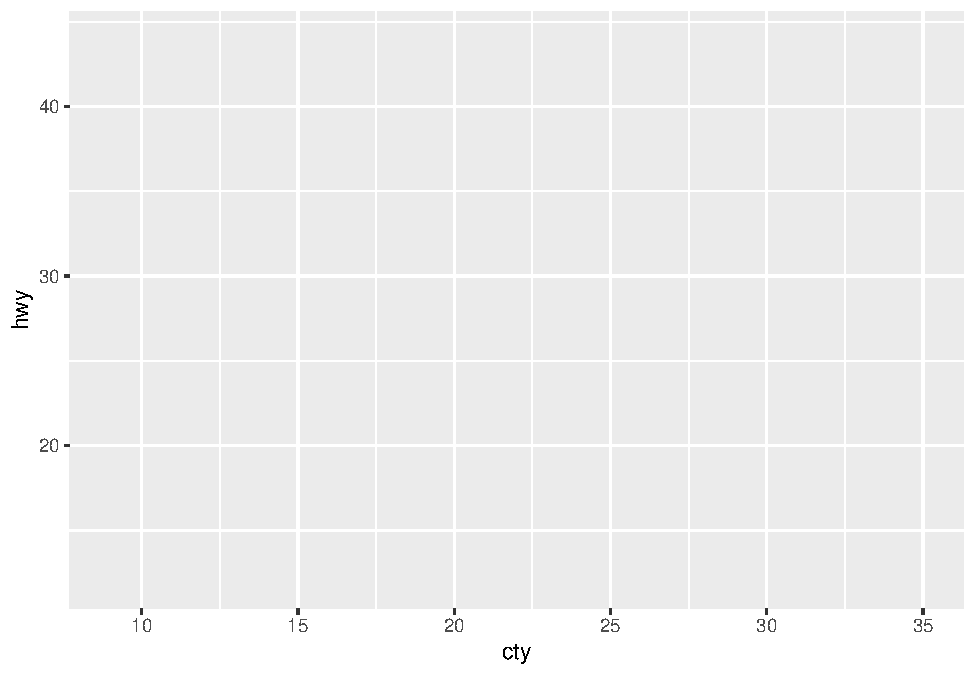
\includegraphics{02_ggplot2_files/figure-latex/unnamed-chunk-3-2.pdf}

\begin{Shaded}
\begin{Highlighting}[]
\CommentTok{\# Alternativas}
\FunctionTok{ggplot}\NormalTok{(dados, }\FunctionTok{aes}\NormalTok{(}\AttributeTok{x =}\NormalTok{ cty, }\AttributeTok{y =}\NormalTok{ hwy)) }\SpecialCharTok{+} 
  \FunctionTok{geom\_point}\NormalTok{()}
\end{Highlighting}
\end{Shaded}

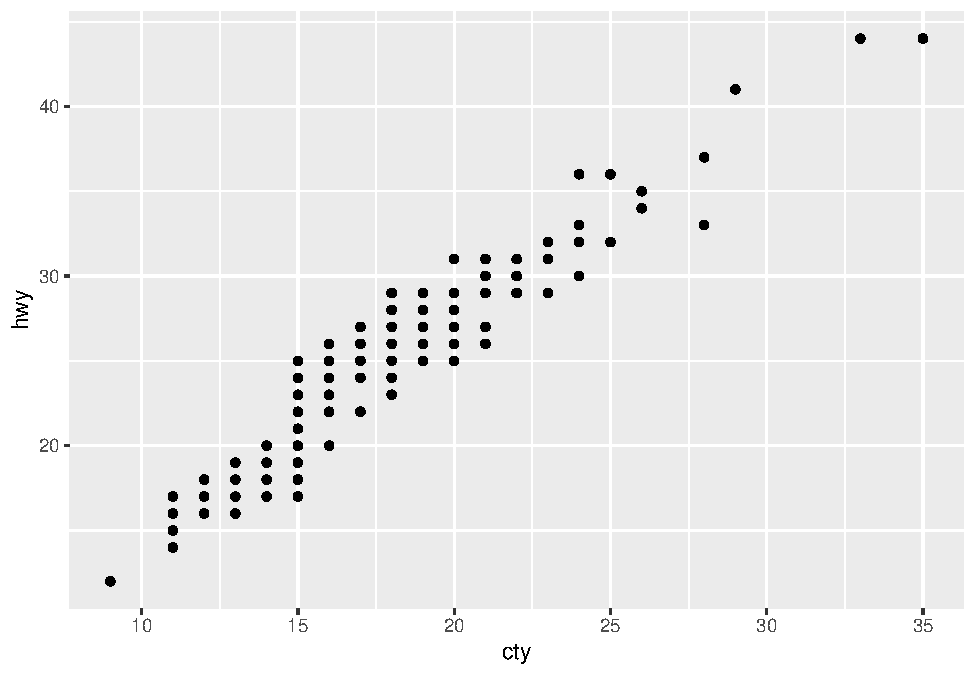
\includegraphics{02_ggplot2_files/figure-latex/unnamed-chunk-3-3.pdf}

\begin{Shaded}
\begin{Highlighting}[]
\FunctionTok{ggplot}\NormalTok{(dados) }\SpecialCharTok{+} 
  \FunctionTok{geom\_point}\NormalTok{(}\FunctionTok{aes}\NormalTok{(}\AttributeTok{x =}\NormalTok{ cty, }\AttributeTok{y =}\NormalTok{ hwy))}
\end{Highlighting}
\end{Shaded}

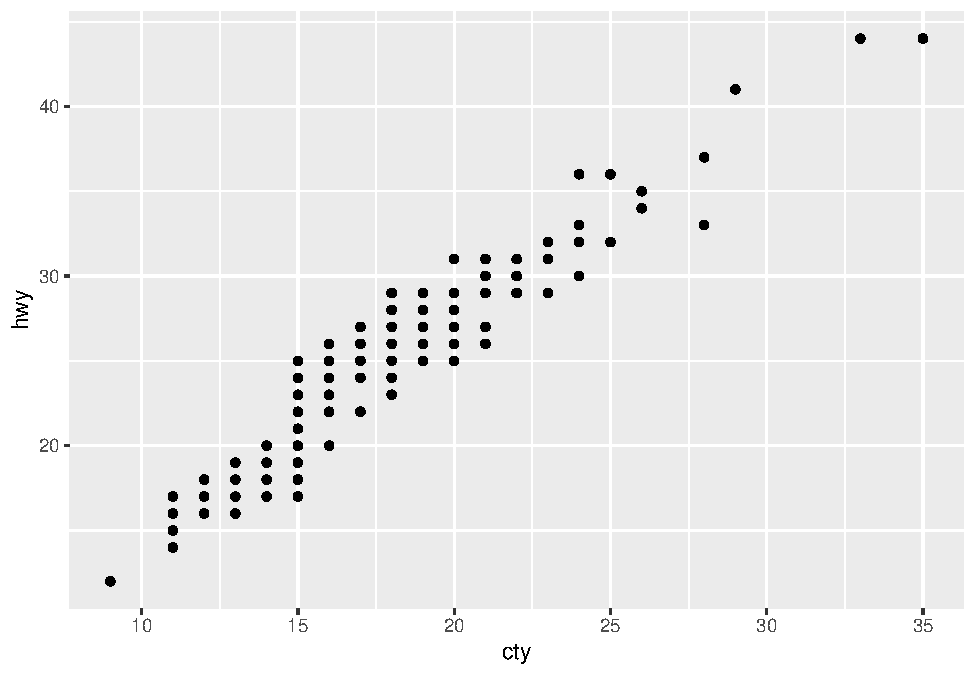
\includegraphics{02_ggplot2_files/figure-latex/unnamed-chunk-3-4.pdf}

\begin{Shaded}
\begin{Highlighting}[]
\FunctionTok{ggplot}\NormalTok{() }\SpecialCharTok{+} 
  \FunctionTok{geom\_point}\NormalTok{(}\AttributeTok{data =}\NormalTok{ dados, }\FunctionTok{aes}\NormalTok{(}\AttributeTok{x =}\NormalTok{ cty, }\AttributeTok{y =}\NormalTok{ hwy))}
\end{Highlighting}
\end{Shaded}

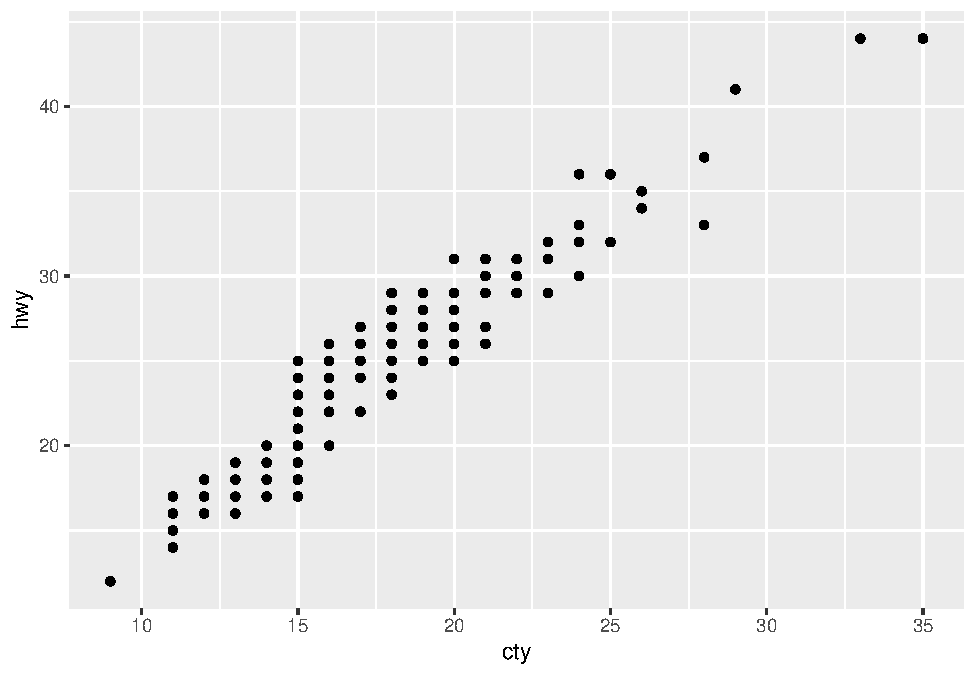
\includegraphics{02_ggplot2_files/figure-latex/unnamed-chunk-3-5.pdf}

\begin{Shaded}
\begin{Highlighting}[]
\CommentTok{\# Fim }

\FunctionTok{ggplot}\NormalTok{(dados, }\FunctionTok{aes}\NormalTok{(}\AttributeTok{x =}\NormalTok{ cty, }\AttributeTok{y =}\NormalTok{ hwy)) }\SpecialCharTok{+} 
  \FunctionTok{geom\_point}\NormalTok{(}\AttributeTok{colour =} \StringTok{"red"}\NormalTok{)}
\end{Highlighting}
\end{Shaded}

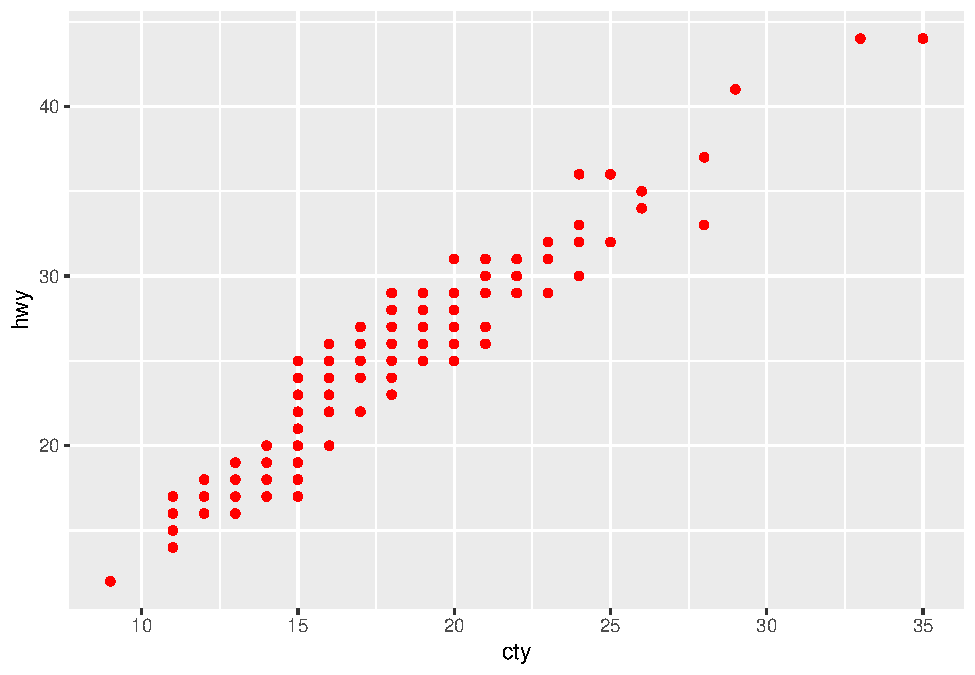
\includegraphics{02_ggplot2_files/figure-latex/unnamed-chunk-3-6.pdf}

\begin{Shaded}
\begin{Highlighting}[]
\FunctionTok{ggplot}\NormalTok{(dados, }\FunctionTok{aes}\NormalTok{(}\AttributeTok{x =}\NormalTok{ cty, }\AttributeTok{y =}\NormalTok{ hwy)) }\SpecialCharTok{+} 
  \FunctionTok{geom\_point}\NormalTok{(}\AttributeTok{colour =} \StringTok{"red"}\NormalTok{, }\AttributeTok{size =} \DecValTok{6}\NormalTok{)}
\end{Highlighting}
\end{Shaded}

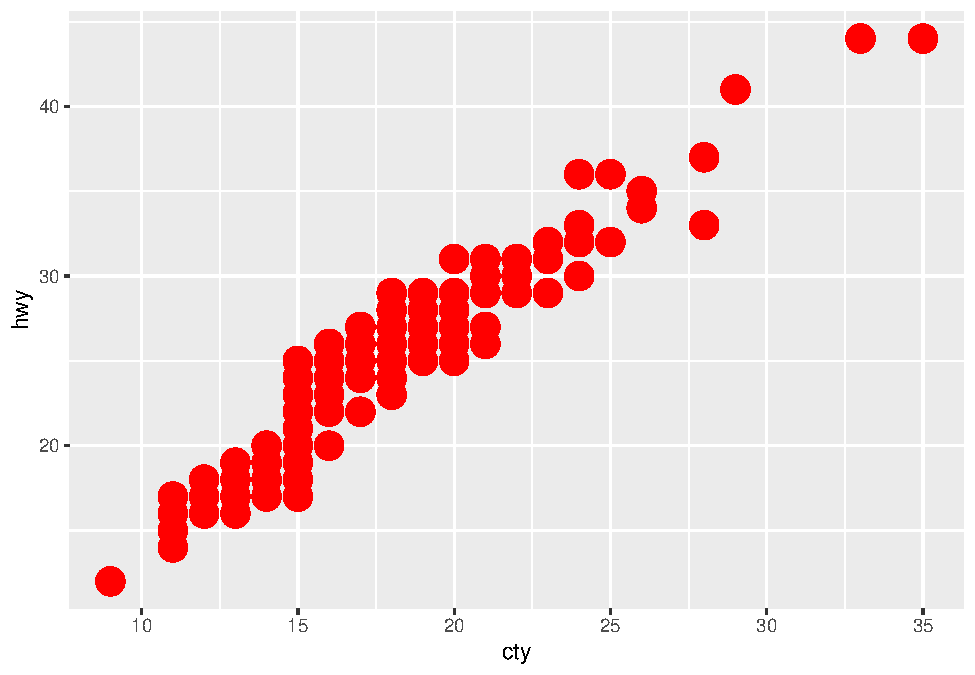
\includegraphics{02_ggplot2_files/figure-latex/unnamed-chunk-3-7.pdf}

\begin{Shaded}
\begin{Highlighting}[]
\FunctionTok{ggplot}\NormalTok{(dados, }\FunctionTok{aes}\NormalTok{(}\AttributeTok{x =}\NormalTok{ cty, }\AttributeTok{y =}\NormalTok{ hwy)) }\SpecialCharTok{+} 
  \FunctionTok{geom\_point}\NormalTok{(}\AttributeTok{colour =} \StringTok{"red"}\NormalTok{, }\AttributeTok{size =} \DecValTok{6}\NormalTok{, }\AttributeTok{shape =} \DecValTok{10}\NormalTok{)}
\end{Highlighting}
\end{Shaded}

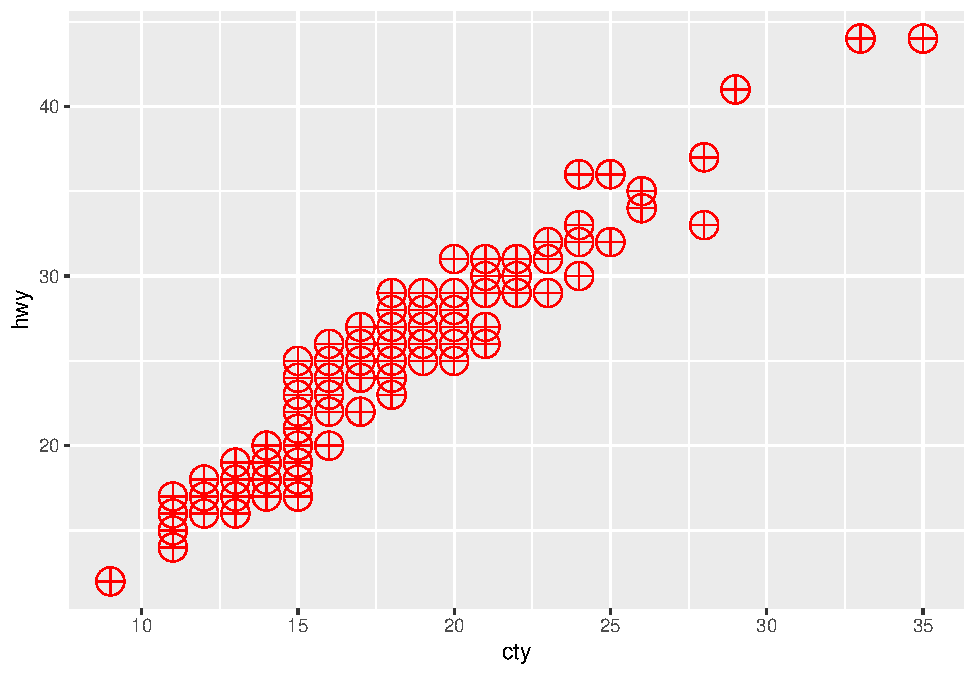
\includegraphics{02_ggplot2_files/figure-latex/unnamed-chunk-3-8.pdf}

\begin{Shaded}
\begin{Highlighting}[]
\CommentTok{\# Alternativa}
\FunctionTok{ggplot}\NormalTok{(dados, }\FunctionTok{aes}\NormalTok{(}\AttributeTok{x =}\NormalTok{ cty, }\AttributeTok{y =}\NormalTok{ hwy)) }\SpecialCharTok{+} 
  \FunctionTok{geom\_point}\NormalTok{(}\AttributeTok{colour =} \StringTok{"red"}\NormalTok{, }\AttributeTok{size =} \DecValTok{6}\NormalTok{, }\AttributeTok{shape =} \StringTok{"circle plus"}\NormalTok{)}
\end{Highlighting}
\end{Shaded}

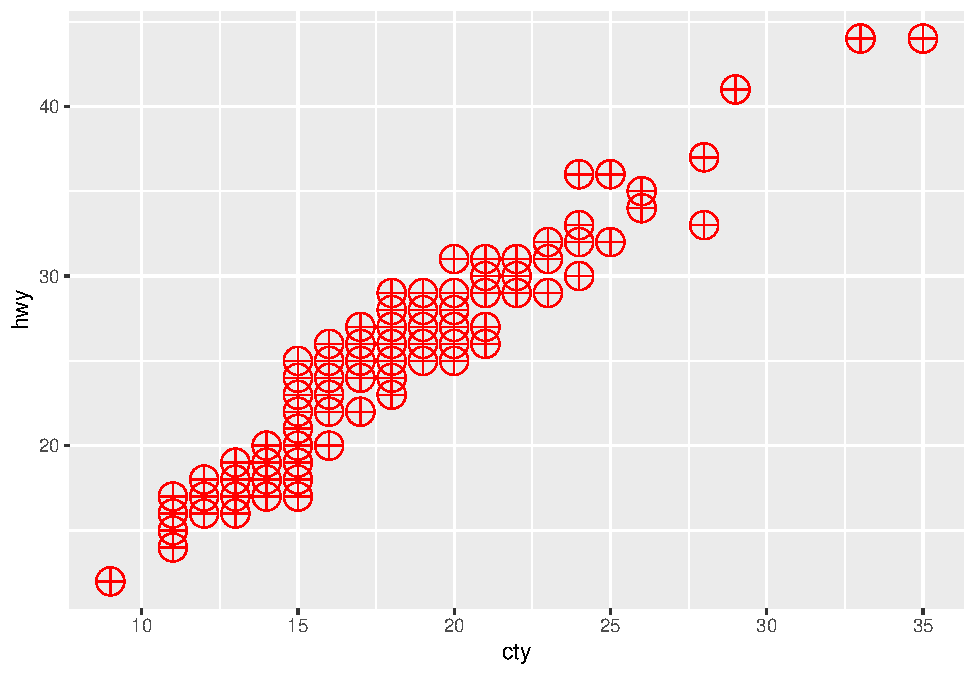
\includegraphics{02_ggplot2_files/figure-latex/unnamed-chunk-3-9.pdf}

\begin{Shaded}
\begin{Highlighting}[]
\FunctionTok{ggplot}\NormalTok{(dados, }\FunctionTok{aes}\NormalTok{(}\AttributeTok{x =}\NormalTok{ cty, }\AttributeTok{y =}\NormalTok{ hwy)) }\SpecialCharTok{+} 
  \FunctionTok{geom\_point}\NormalTok{(}\AttributeTok{colour =} \StringTok{"red"}\NormalTok{, }\AttributeTok{size =} \DecValTok{6}\NormalTok{, }\AttributeTok{shape =} \DecValTok{10}\NormalTok{)}\SpecialCharTok{+}
  \FunctionTok{labs}\NormalTok{(}\AttributeTok{x =} \StringTok{"cty (city miles per gallon hwy)"}\NormalTok{, }
       \AttributeTok{y =} \StringTok{"hwy (highway miles per gallon)"}\NormalTok{, }
       \AttributeTok{title =} \StringTok{"Pensar em algum título..."}\NormalTok{, }
       \AttributeTok{subtitle =} \StringTok{"Escrever alguma coisa"}\NormalTok{)}
\end{Highlighting}
\end{Shaded}

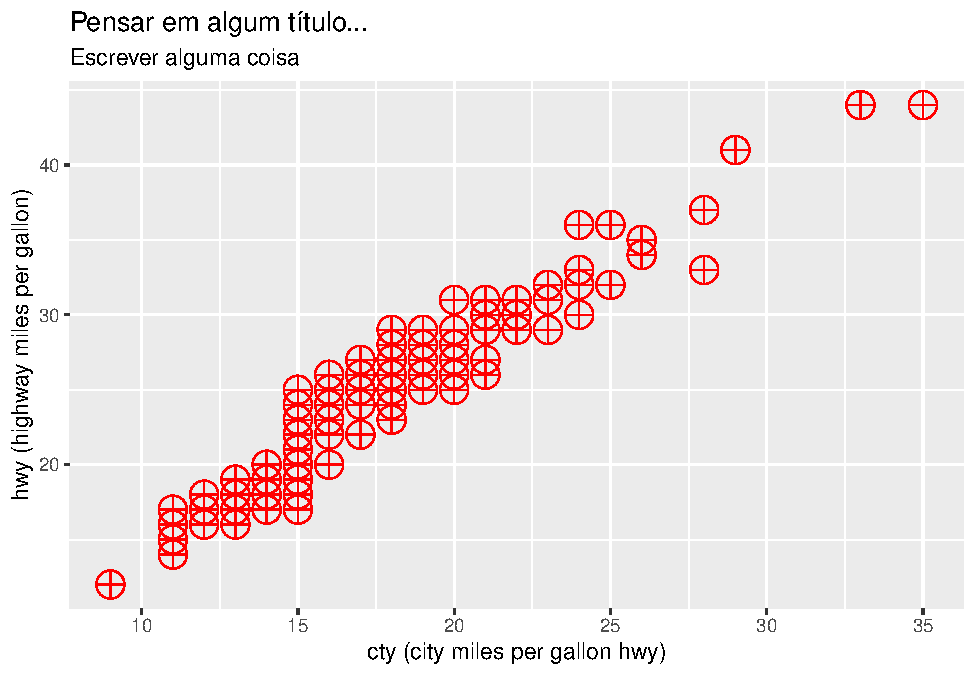
\includegraphics{02_ggplot2_files/figure-latex/unnamed-chunk-3-10.pdf}

\hypertarget{mais-detalhes-sobre-geom_point}{%
\subsection{Mais detalhes sobre geom\_point}\label{mais-detalhes-sobre-geom_point}}

\begin{quote}
geom\_point() understands the following aesthetics (required aesthetics are in bold):
\end{quote}

\begin{itemize}
\item
  x
\item
  y
\item
  alpha
\item
  colour
\item
  fill
\item
  group
\item
  shape
\item
  size
\item
  stroke
\end{itemize}

\begin{Shaded}
\begin{Highlighting}[]
\FunctionTok{ggplot}\NormalTok{(dados, }\FunctionTok{aes}\NormalTok{(}\AttributeTok{x =}\NormalTok{ cty, }\AttributeTok{y =}\NormalTok{ hwy)) }\SpecialCharTok{+} 
  \FunctionTok{geom\_point}\NormalTok{()}
\end{Highlighting}
\end{Shaded}

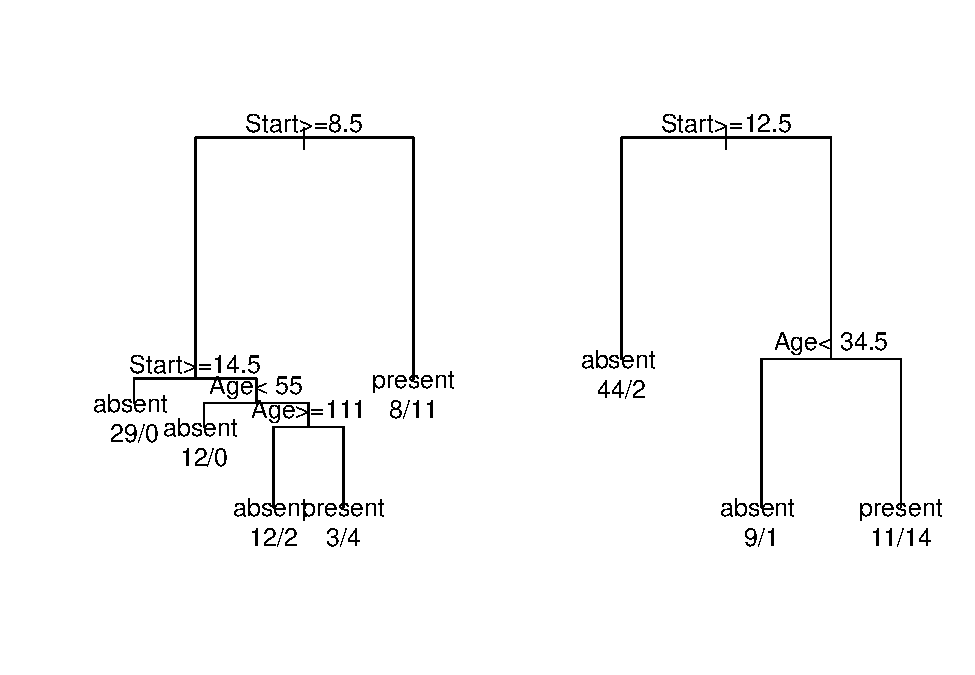
\includegraphics{02_ggplot2_files/figure-latex/unnamed-chunk-4-1.pdf}

\begin{Shaded}
\begin{Highlighting}[]
\FunctionTok{ggplot}\NormalTok{(dados, }\FunctionTok{aes}\NormalTok{(}\AttributeTok{x =}\NormalTok{ cty, }\AttributeTok{y =}\NormalTok{ hwy, }\AttributeTok{col =} \FunctionTok{factor}\NormalTok{(year))) }\SpecialCharTok{+} 
  \FunctionTok{geom\_point}\NormalTok{() }\SpecialCharTok{+} 
  \FunctionTok{labs}\NormalTok{(}\AttributeTok{col =} \StringTok{"year"}\NormalTok{)}
\end{Highlighting}
\end{Shaded}

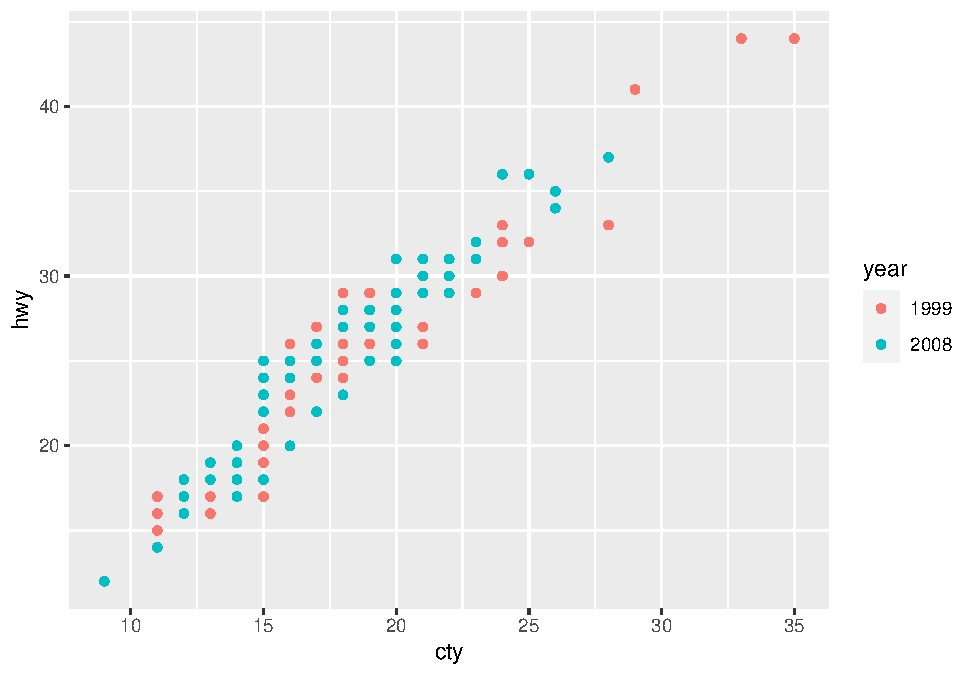
\includegraphics{02_ggplot2_files/figure-latex/unnamed-chunk-4-2.pdf}

\begin{Shaded}
\begin{Highlighting}[]
\CommentTok{\# Alternativa}
\FunctionTok{ggplot}\NormalTok{(dados, }\FunctionTok{aes}\NormalTok{(}\AttributeTok{x =}\NormalTok{ cty, }\AttributeTok{y =}\NormalTok{ hwy, }\AttributeTok{col =} \FunctionTok{factor}\NormalTok{(class))) }\SpecialCharTok{+} 
  \FunctionTok{geom\_point}\NormalTok{() }\SpecialCharTok{+} 
  \FunctionTok{labs}\NormalTok{(}\AttributeTok{col =} \StringTok{"class"}\NormalTok{)}\SpecialCharTok{+}
  \FunctionTok{scale\_color\_brewer}\NormalTok{(}\AttributeTok{type =} \StringTok{"qual"}\NormalTok{)}
\end{Highlighting}
\end{Shaded}

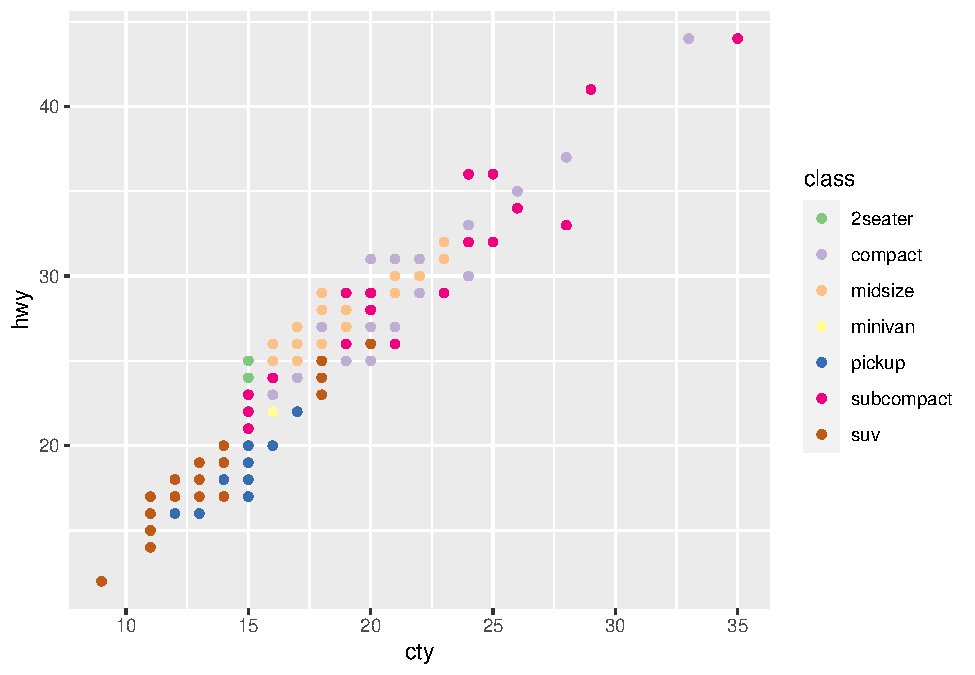
\includegraphics{02_ggplot2_files/figure-latex/unnamed-chunk-4-3.pdf}

\begin{Shaded}
\begin{Highlighting}[]
\FunctionTok{ggplot}\NormalTok{(dados, }\FunctionTok{aes}\NormalTok{(}\AttributeTok{x =}\NormalTok{ cty, }\AttributeTok{y =}\NormalTok{ hwy, }\AttributeTok{col =} \FunctionTok{factor}\NormalTok{(class))) }\SpecialCharTok{+} 
  \FunctionTok{geom\_point}\NormalTok{() }\SpecialCharTok{+} 
  \FunctionTok{labs}\NormalTok{(}\AttributeTok{col =} \StringTok{"class"}\NormalTok{)}\SpecialCharTok{+}
  \FunctionTok{scale\_color\_brewer}\NormalTok{(}\AttributeTok{type =} \StringTok{"div"}\NormalTok{)}
\end{Highlighting}
\end{Shaded}

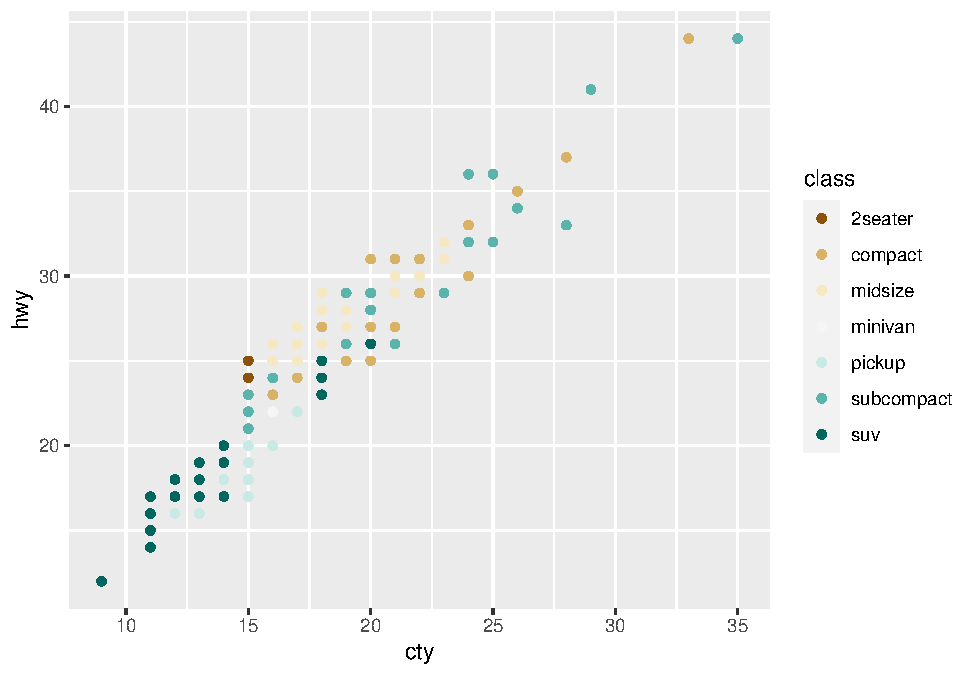
\includegraphics{02_ggplot2_files/figure-latex/unnamed-chunk-4-4.pdf}

\begin{Shaded}
\begin{Highlighting}[]
\FunctionTok{ggplot}\NormalTok{(dados, }\FunctionTok{aes}\NormalTok{(}\AttributeTok{x =}\NormalTok{ cty, }\AttributeTok{y =}\NormalTok{ hwy, }\AttributeTok{col =} \FunctionTok{factor}\NormalTok{(class))) }\SpecialCharTok{+} 
  \FunctionTok{geom\_point}\NormalTok{() }\SpecialCharTok{+} 
  \FunctionTok{labs}\NormalTok{(}\AttributeTok{col =} \StringTok{"class"}\NormalTok{)}\SpecialCharTok{+}
  \FunctionTok{scale\_color\_brewer}\NormalTok{(}\AttributeTok{palette =} \StringTok{"Set1"}\NormalTok{, }\AttributeTok{name =} \StringTok{"Tipo de carro"}\NormalTok{)}\SpecialCharTok{+}
  \FunctionTok{scale\_y\_continuous}\NormalTok{(}\AttributeTok{breaks =} \FunctionTok{seq}\NormalTok{(}\DecValTok{10}\NormalTok{,}\DecValTok{60}\NormalTok{,}\DecValTok{3}\NormalTok{))}\SpecialCharTok{+}
  \FunctionTok{scale\_x\_continuous}\NormalTok{(}\AttributeTok{breaks =} \FunctionTok{seq}\NormalTok{(}\DecValTok{10}\NormalTok{,}\DecValTok{40}\NormalTok{,}\DecValTok{3}\NormalTok{))}\SpecialCharTok{+}
  \FunctionTok{theme\_minimal}\NormalTok{()}
\end{Highlighting}
\end{Shaded}

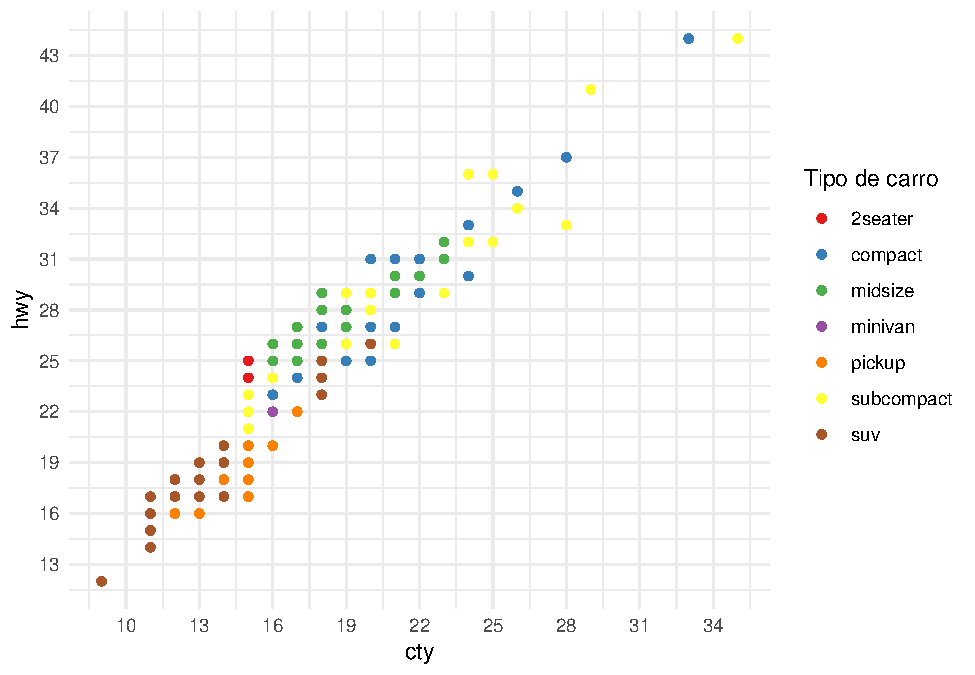
\includegraphics{02_ggplot2_files/figure-latex/unnamed-chunk-4-5.pdf}

\begin{Shaded}
\begin{Highlighting}[]
\FunctionTok{ggplot}\NormalTok{(dados, }\FunctionTok{aes}\NormalTok{(}\AttributeTok{x =}\NormalTok{ cty, }\AttributeTok{y =}\NormalTok{ hwy, }\AttributeTok{alpha =} \FunctionTok{factor}\NormalTok{(year))) }\SpecialCharTok{+} 
  \FunctionTok{geom\_point}\NormalTok{() }\SpecialCharTok{+} 
  \FunctionTok{labs}\NormalTok{(}\AttributeTok{alpha =} \StringTok{"year"}\NormalTok{)}
\end{Highlighting}
\end{Shaded}

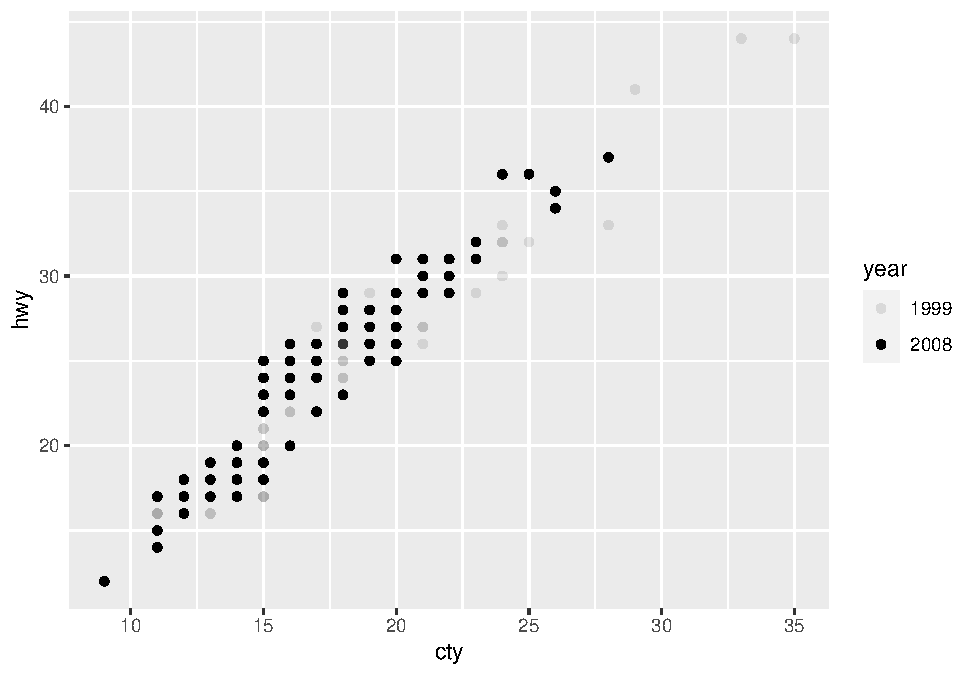
\includegraphics{02_ggplot2_files/figure-latex/unnamed-chunk-4-6.pdf}

\begin{Shaded}
\begin{Highlighting}[]
\FunctionTok{ggplot}\NormalTok{(dados, }\FunctionTok{aes}\NormalTok{(}\AttributeTok{x =}\NormalTok{ cty, }\AttributeTok{y =}\NormalTok{ hwy, }\AttributeTok{size =} \FunctionTok{factor}\NormalTok{(year))) }\SpecialCharTok{+} 
  \FunctionTok{geom\_point}\NormalTok{() }\SpecialCharTok{+} 
  \FunctionTok{labs}\NormalTok{(}\AttributeTok{size =} \StringTok{"year"}\NormalTok{)}
\end{Highlighting}
\end{Shaded}

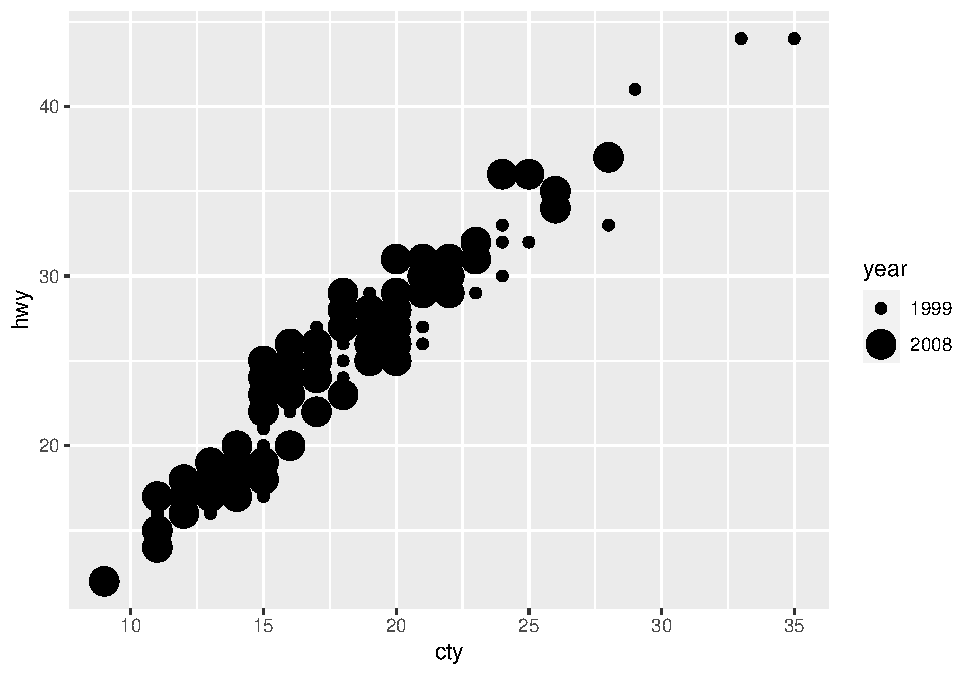
\includegraphics{02_ggplot2_files/figure-latex/unnamed-chunk-4-7.pdf}

\begin{Shaded}
\begin{Highlighting}[]
\CommentTok{\# Alternativa}
\FunctionTok{ggplot}\NormalTok{(dados, }\FunctionTok{aes}\NormalTok{(}\AttributeTok{x =}\NormalTok{ cty, }\AttributeTok{y =}\NormalTok{ hwy, }\AttributeTok{col =}\NormalTok{ cty }\SpecialCharTok{\textless{}=} \DecValTok{20}\NormalTok{)) }\SpecialCharTok{+} 
  \FunctionTok{geom\_point}\NormalTok{() }\SpecialCharTok{+} 
  \FunctionTok{geom\_vline}\NormalTok{(}\AttributeTok{xintercept =} \DecValTok{20}\NormalTok{)}\SpecialCharTok{+}
  \FunctionTok{labs}\NormalTok{(}\AttributeTok{col =} \StringTok{"year"}\NormalTok{)}
\end{Highlighting}
\end{Shaded}

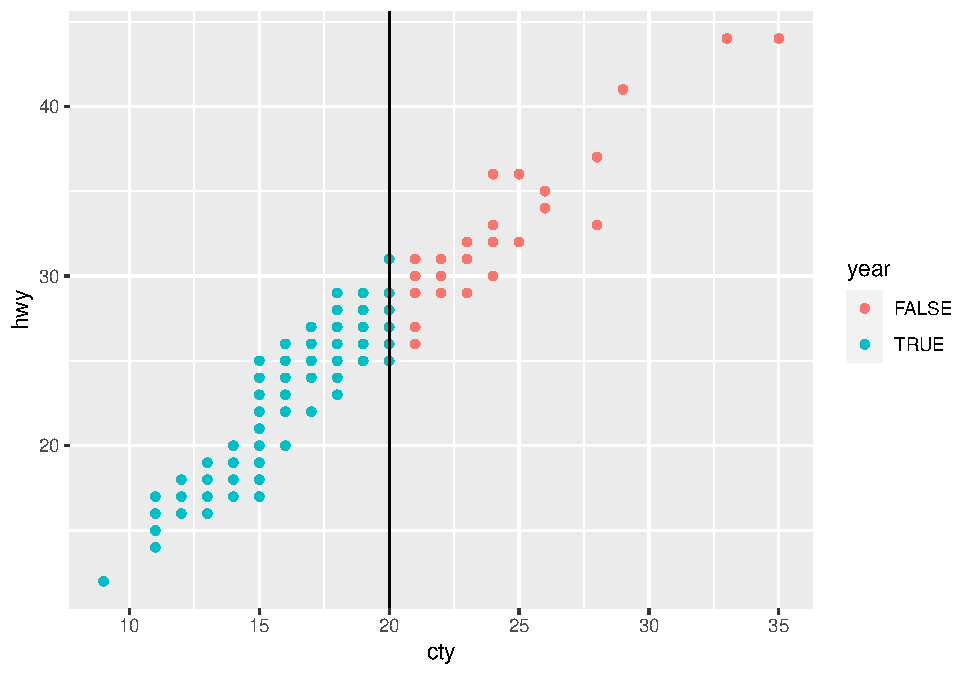
\includegraphics{02_ggplot2_files/figure-latex/unnamed-chunk-4-8.pdf}

\begin{Shaded}
\begin{Highlighting}[]
\CommentTok{\# Erro comum}
\FunctionTok{ggplot}\NormalTok{(dados, }\FunctionTok{aes}\NormalTok{(}\AttributeTok{x =}\NormalTok{ cty, }\AttributeTok{y =}\NormalTok{ hwy, }\AttributeTok{col =} \StringTok{"red"}\NormalTok{)) }\SpecialCharTok{+} 
  \FunctionTok{geom\_point}\NormalTok{()}\SpecialCharTok{+}
  \FunctionTok{labs}\NormalTok{(}\AttributeTok{col =} \StringTok{"year"}\NormalTok{)}
\end{Highlighting}
\end{Shaded}

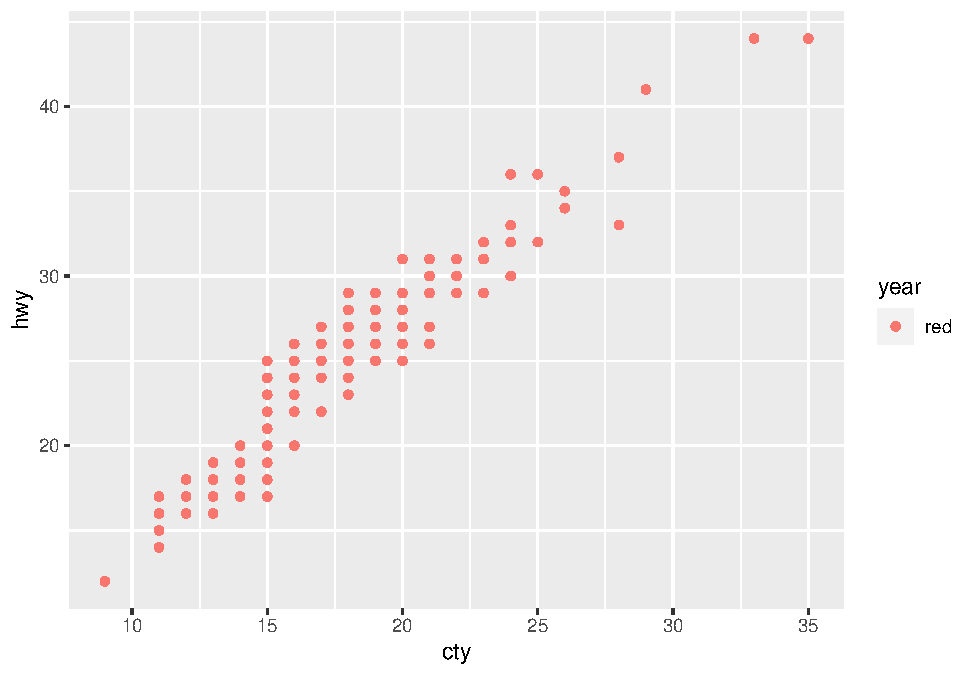
\includegraphics{02_ggplot2_files/figure-latex/unnamed-chunk-4-9.pdf}

\begin{Shaded}
\begin{Highlighting}[]
\FunctionTok{ggplot}\NormalTok{(dados, }\FunctionTok{aes}\NormalTok{(}\AttributeTok{x =}\NormalTok{ cty, }\AttributeTok{y =}\NormalTok{ hwy)) }\SpecialCharTok{+} 
  \FunctionTok{geom\_point}\NormalTok{(}\AttributeTok{col =} \StringTok{"red"}\NormalTok{)}\SpecialCharTok{+}
  \FunctionTok{labs}\NormalTok{(}\AttributeTok{col =} \StringTok{"year"}\NormalTok{)}
\end{Highlighting}
\end{Shaded}

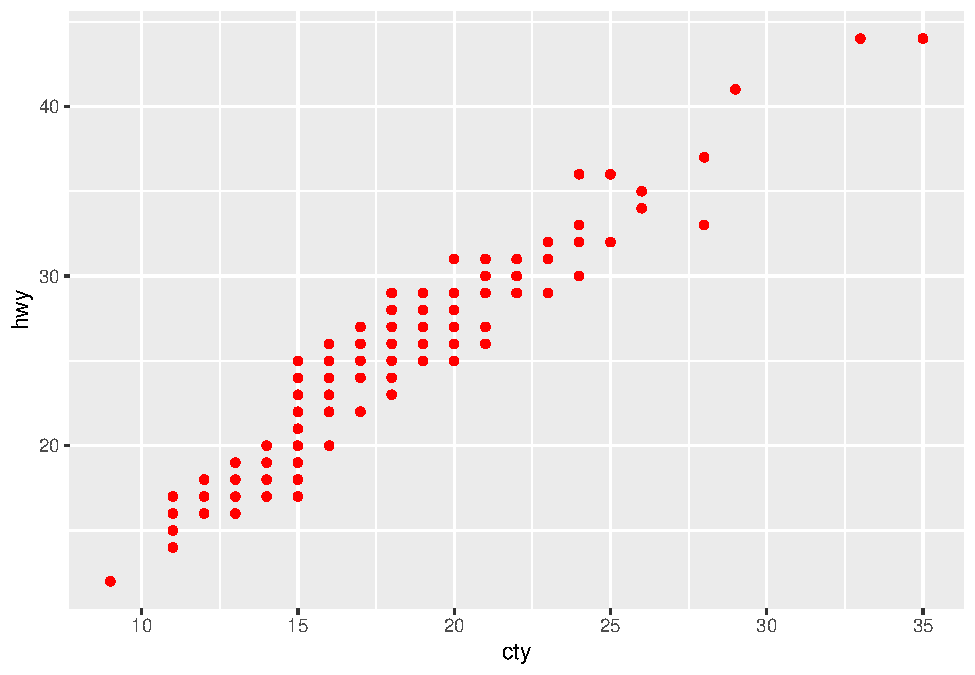
\includegraphics{02_ggplot2_files/figure-latex/unnamed-chunk-4-10.pdf}

\begin{Shaded}
\begin{Highlighting}[]
\CommentTok{\# Fim  Erro comum}

\FunctionTok{ggplot}\NormalTok{(dados, }\FunctionTok{aes}\NormalTok{(}\AttributeTok{x =}\NormalTok{ cty, }\AttributeTok{y =}\NormalTok{ hwy, }\AttributeTok{shape =} \FunctionTok{factor}\NormalTok{(year))) }\SpecialCharTok{+} 
  \FunctionTok{geom\_point}\NormalTok{(}\AttributeTok{col =} \StringTok{"red"}\NormalTok{) }\SpecialCharTok{+} 
  \FunctionTok{labs}\NormalTok{(}\AttributeTok{shape =} \StringTok{"year"}\NormalTok{)}
\end{Highlighting}
\end{Shaded}

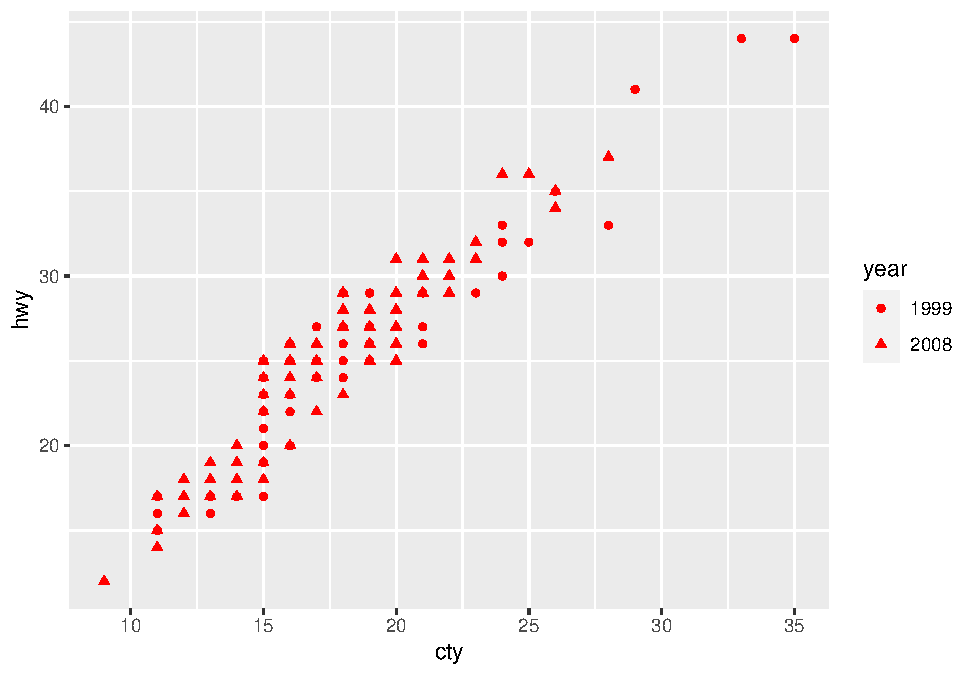
\includegraphics{02_ggplot2_files/figure-latex/unnamed-chunk-4-11.pdf}

\begin{Shaded}
\begin{Highlighting}[]
\FunctionTok{ggplot}\NormalTok{(dados, }\FunctionTok{aes}\NormalTok{(}\AttributeTok{x =}\NormalTok{ cty, }\AttributeTok{y =}\NormalTok{ hwy, }\AttributeTok{size =}\NormalTok{ class)) }\SpecialCharTok{+} 
  \FunctionTok{geom\_point}\NormalTok{() }\SpecialCharTok{+} 
  \FunctionTok{labs}\NormalTok{(}\AttributeTok{size =} \StringTok{"class"}\NormalTok{)}
\end{Highlighting}
\end{Shaded}

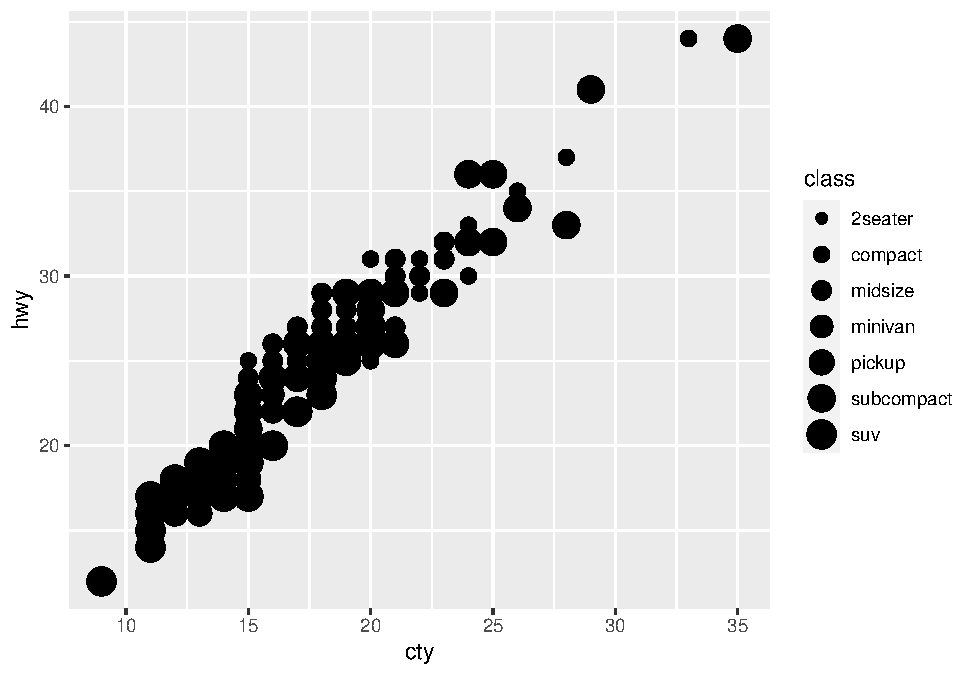
\includegraphics{02_ggplot2_files/figure-latex/unnamed-chunk-4-12.pdf}

\begin{Shaded}
\begin{Highlighting}[]
\FunctionTok{ggplot}\NormalTok{(dados, }\FunctionTok{aes}\NormalTok{(}\AttributeTok{x =}\NormalTok{ cty, }\AttributeTok{y =}\NormalTok{ hwy, }
                  \AttributeTok{size =}\NormalTok{ class, }
                  \AttributeTok{col =}\NormalTok{ class)) }\SpecialCharTok{+} 
  \FunctionTok{geom\_point}\NormalTok{() }\SpecialCharTok{+} 
  \FunctionTok{guides}\NormalTok{(}\AttributeTok{colour =} \FunctionTok{guide\_legend}\NormalTok{(}\StringTok{"Tipo de carro (color)"}\NormalTok{),}
         \AttributeTok{size =} \FunctionTok{guide\_legend}\NormalTok{(}\StringTok{"Tipo de carro (size)"}\NormalTok{))}
\end{Highlighting}
\end{Shaded}

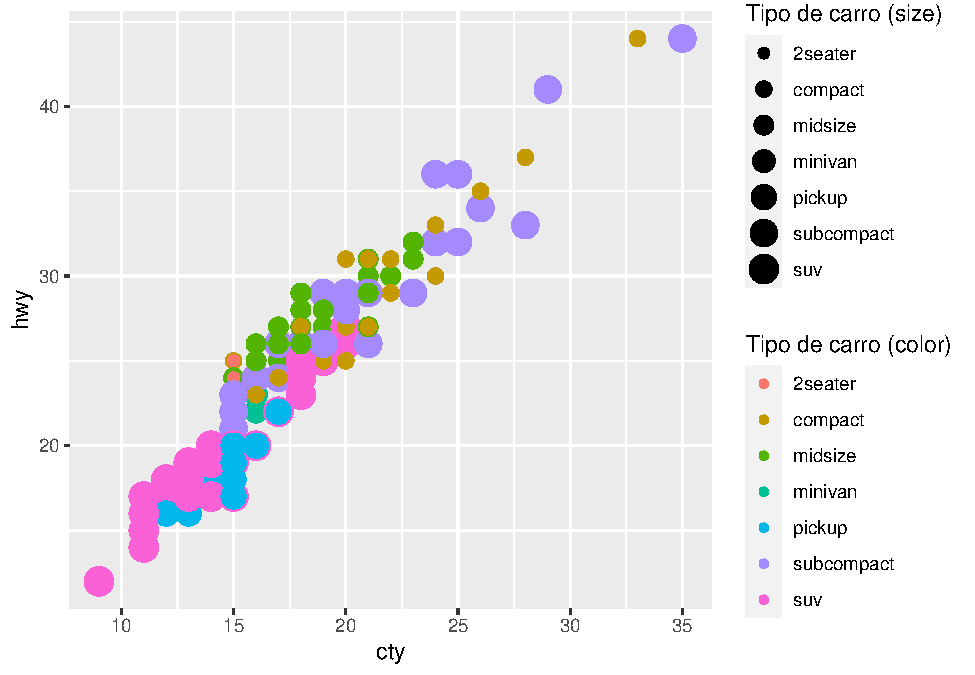
\includegraphics{02_ggplot2_files/figure-latex/unnamed-chunk-4-13.pdf}

\begin{Shaded}
\begin{Highlighting}[]
\FunctionTok{ggplot}\NormalTok{(dados, }\FunctionTok{aes}\NormalTok{(}\AttributeTok{x =}\NormalTok{ cty, }\AttributeTok{y =}\NormalTok{ hwy, }
                  \AttributeTok{size =}\NormalTok{ class, }
                  \AttributeTok{col =}\NormalTok{ class)) }\SpecialCharTok{+} 
  \FunctionTok{geom\_point}\NormalTok{() }\SpecialCharTok{+} 
  \FunctionTok{labs}\NormalTok{(}\AttributeTok{col =} \StringTok{"Tipo de Carro"}\NormalTok{, }\AttributeTok{size =} \StringTok{"Tipo de Carro"}\NormalTok{)}\SpecialCharTok{+}
  \FunctionTok{guides}\NormalTok{(}\AttributeTok{col =} \StringTok{"legend"}\NormalTok{)}
\end{Highlighting}
\end{Shaded}

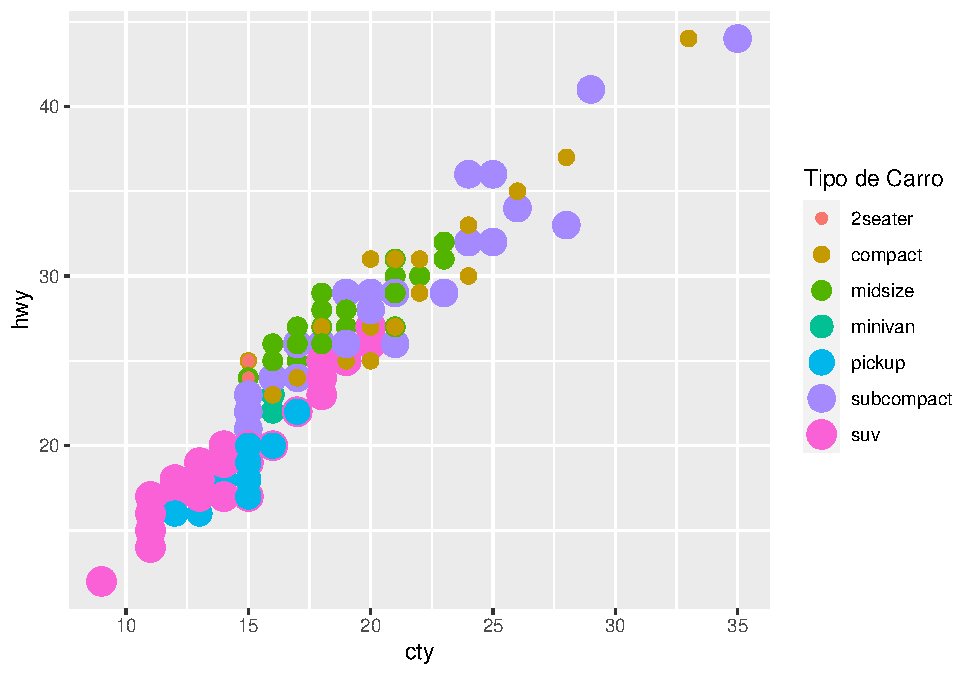
\includegraphics{02_ggplot2_files/figure-latex/unnamed-chunk-4-14.pdf}

\hypertarget{smooth-boxplot-histogram}{%
\section{smooth, boxplot, histogram}\label{smooth-boxplot-histogram}}

\begin{Shaded}
\begin{Highlighting}[]
\NormalTok{v1}\OtherTok{\textless{}{-}} \FunctionTok{ggplot}\NormalTok{(dados, }\FunctionTok{aes}\NormalTok{(}\AttributeTok{x =}\NormalTok{ cty, }\AttributeTok{y =}\NormalTok{ hwy)) }\SpecialCharTok{+} 
  \FunctionTok{geom\_point}\NormalTok{(}\AttributeTok{col =} \StringTok{"blue"}\NormalTok{)}\SpecialCharTok{+}
  \FunctionTok{geom\_smooth}\NormalTok{(}\AttributeTok{method =}\NormalTok{ mgcv}\SpecialCharTok{::}\NormalTok{gam,}
              \AttributeTok{formula =}\NormalTok{ y }\SpecialCharTok{\textasciitilde{}} \FunctionTok{s}\NormalTok{(x, }\AttributeTok{bs =} \StringTok{"cs"}\NormalTok{) ,}
              \AttributeTok{col =} \StringTok{"red"}\NormalTok{, }
              \AttributeTok{se =} \ConstantTok{FALSE}\NormalTok{)}
\NormalTok{v1}
\end{Highlighting}
\end{Shaded}

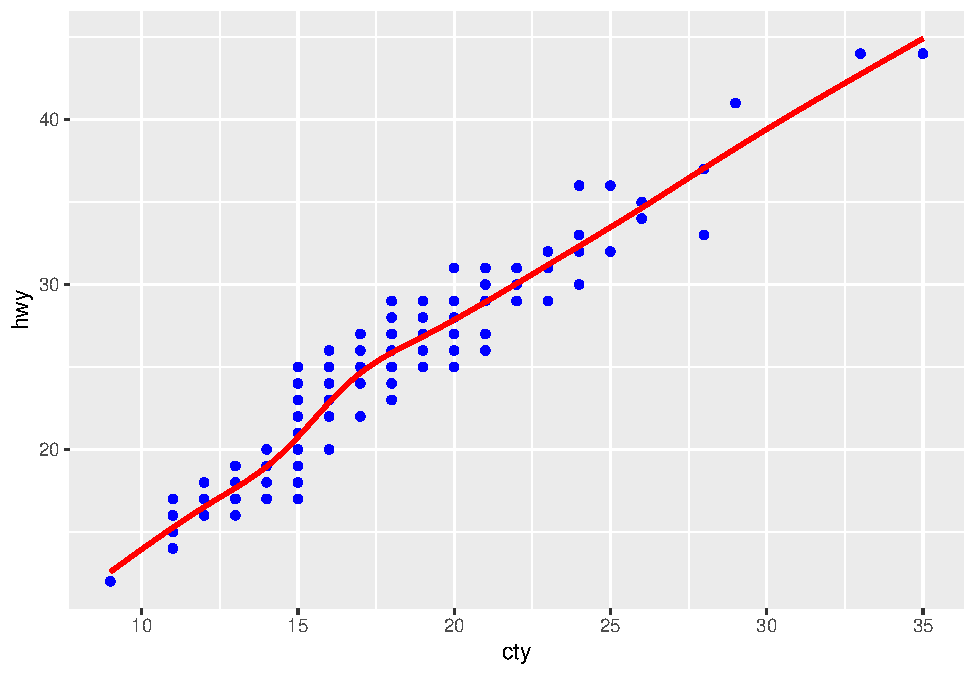
\includegraphics{02_ggplot2_files/figure-latex/unnamed-chunk-5-1.pdf}

\begin{Shaded}
\begin{Highlighting}[]
\NormalTok{v2 }\OtherTok{\textless{}{-}} \FunctionTok{ggplot}\NormalTok{(dados, }\FunctionTok{aes}\NormalTok{(}\AttributeTok{x =}\NormalTok{ cty)) }\SpecialCharTok{+} 
  \FunctionTok{geom\_boxplot}\NormalTok{(}\AttributeTok{fill =} \StringTok{"red"}\NormalTok{)}
\NormalTok{v2}
\end{Highlighting}
\end{Shaded}

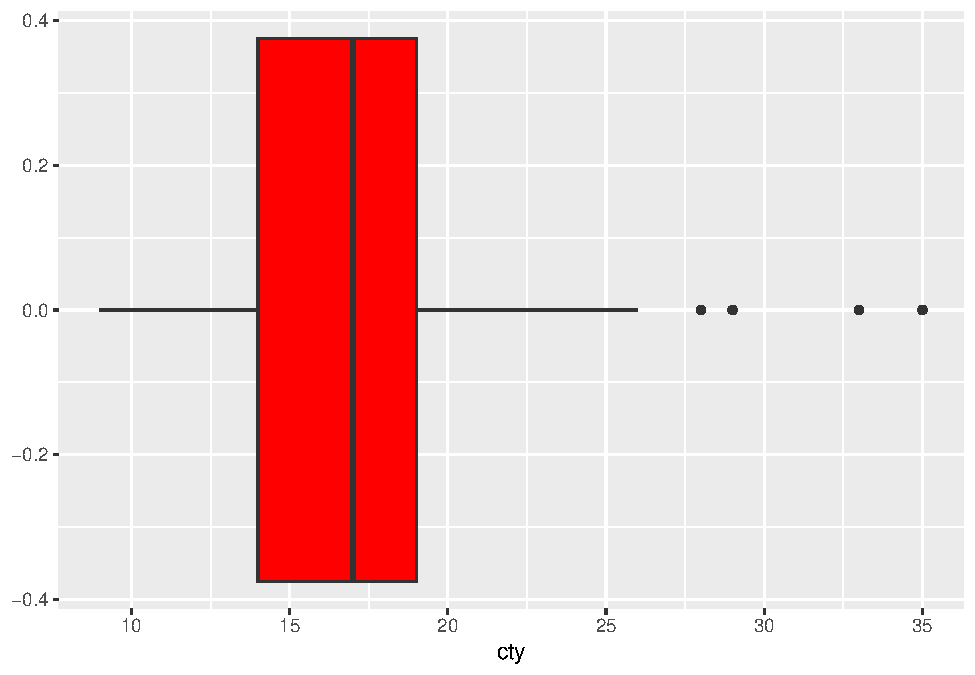
\includegraphics{02_ggplot2_files/figure-latex/unnamed-chunk-5-2.pdf}

\begin{Shaded}
\begin{Highlighting}[]
\NormalTok{v3 }\OtherTok{\textless{}{-}} \FunctionTok{ggplot}\NormalTok{(dados, }\FunctionTok{aes}\NormalTok{(}\AttributeTok{x =}\NormalTok{ cty)) }\SpecialCharTok{+} 
  \FunctionTok{geom\_histogram}\NormalTok{(}\AttributeTok{bins =} \DecValTok{10}\NormalTok{, }\AttributeTok{fill =} \StringTok{"red"}\NormalTok{, }\AttributeTok{col =} \StringTok{"blue"}\NormalTok{, }\AttributeTok{lwd=}\DecValTok{2}\NormalTok{)}
\NormalTok{v3}
\end{Highlighting}
\end{Shaded}

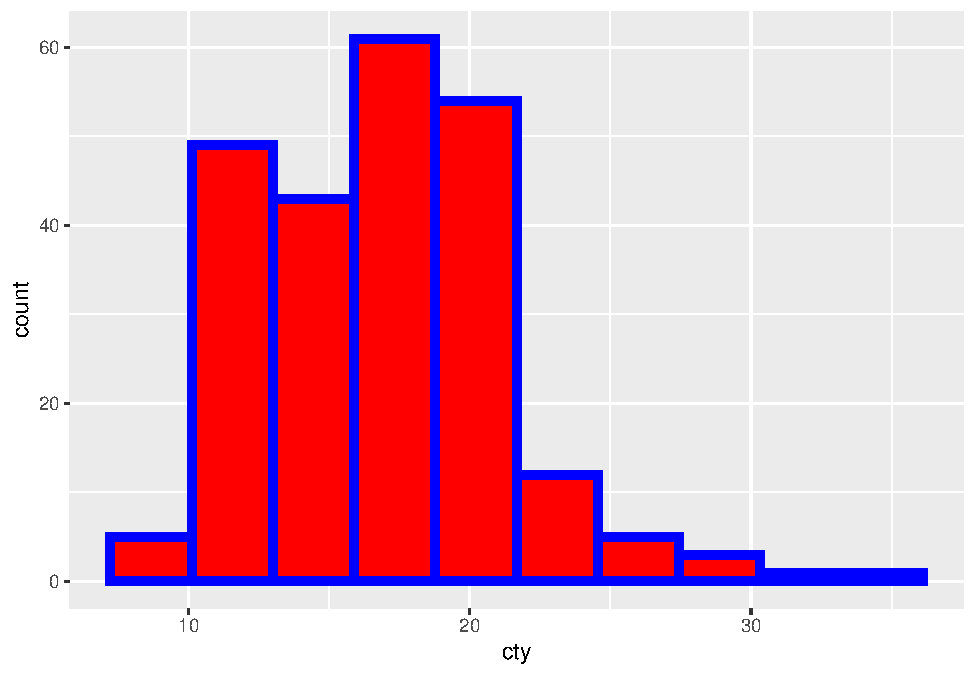
\includegraphics{02_ggplot2_files/figure-latex/unnamed-chunk-5-3.pdf}

\begin{Shaded}
\begin{Highlighting}[]
\NormalTok{v4}\OtherTok{\textless{}{-}} \FunctionTok{ggplot}\NormalTok{(dados, }\FunctionTok{aes}\NormalTok{(}\AttributeTok{x =}\NormalTok{ cty)) }\SpecialCharTok{+} 
  \FunctionTok{geom\_histogram}\NormalTok{(}\FunctionTok{aes}\NormalTok{(}\AttributeTok{y =} \FunctionTok{after\_stat}\NormalTok{(density)),}
                 \AttributeTok{bins =} \DecValTok{10}\NormalTok{, }\AttributeTok{fill =} \StringTok{"yellow"}\NormalTok{, }\AttributeTok{col =} \StringTok{"red"}\NormalTok{) }\SpecialCharTok{+}
  \FunctionTok{geom\_density}\NormalTok{(}\AttributeTok{col =} \StringTok{"blue"}\NormalTok{, }\AttributeTok{lwd =}\DecValTok{3}\NormalTok{)}
\NormalTok{v4}
\end{Highlighting}
\end{Shaded}

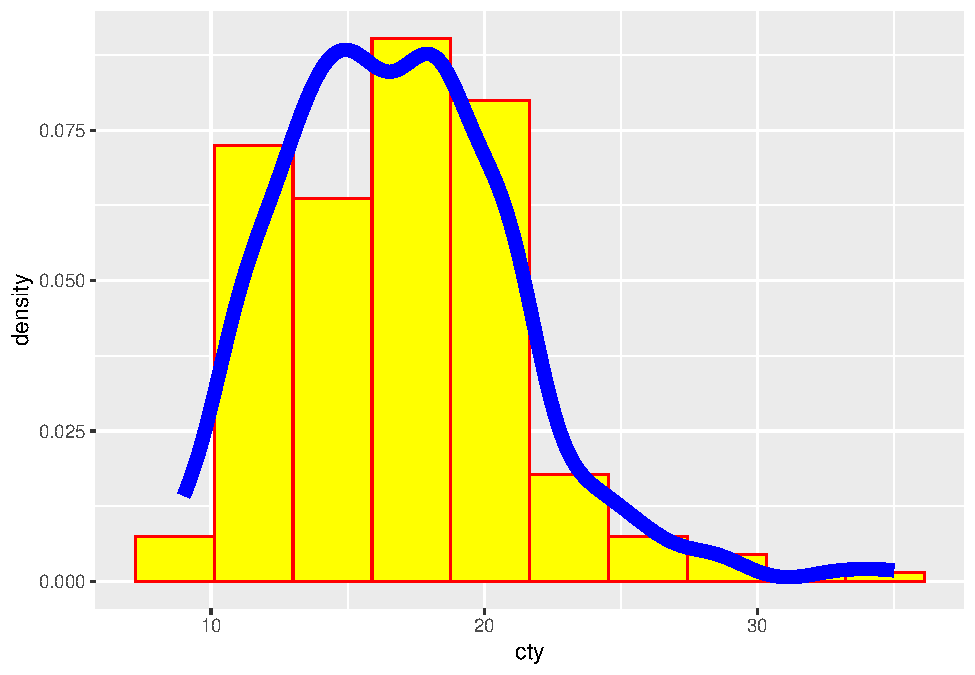
\includegraphics{02_ggplot2_files/figure-latex/unnamed-chunk-5-4.pdf}

\begin{Shaded}
\begin{Highlighting}[]
\CommentTok{\# Adicional (estatístic experimental)}
\FunctionTok{ggplot}\NormalTok{(dados, }\FunctionTok{aes}\NormalTok{(}\AttributeTok{x =}\NormalTok{ drv, }\AttributeTok{y =}\NormalTok{ cty, }\AttributeTok{col =}\NormalTok{ drv)) }\SpecialCharTok{+} 
  \FunctionTok{geom\_boxplot}\NormalTok{()}\SpecialCharTok{+}
  \FunctionTok{theme\_bw}\NormalTok{()}\SpecialCharTok{+}
  \FunctionTok{theme}\NormalTok{(}\AttributeTok{legend.position =} \StringTok{"none"}\NormalTok{)}
\end{Highlighting}
\end{Shaded}

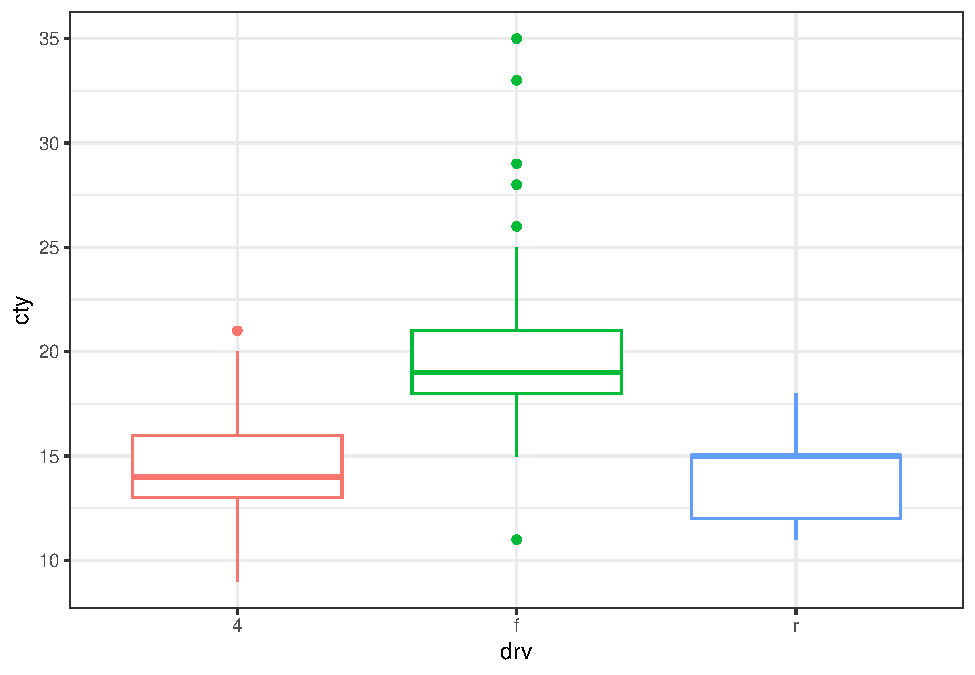
\includegraphics{02_ggplot2_files/figure-latex/unnamed-chunk-5-5.pdf}

\hypertarget{gridextra-e-patchwork}{%
\section{gridExtra e patchwork}\label{gridextra-e-patchwork}}

Alguns links

\href{https://patchwork.data-imaginist.com/articles/guides/assembly.html}{link 1: patchwork}

\href{https://patchwork.data-imaginist.com/articles/patchwork.html}{link 2: patchwork}

\begin{Shaded}
\begin{Highlighting}[]
\CommentTok{\# gridExtra}
\FunctionTok{grid.arrange}\NormalTok{(v1, v2, v3, v4) }
\end{Highlighting}
\end{Shaded}

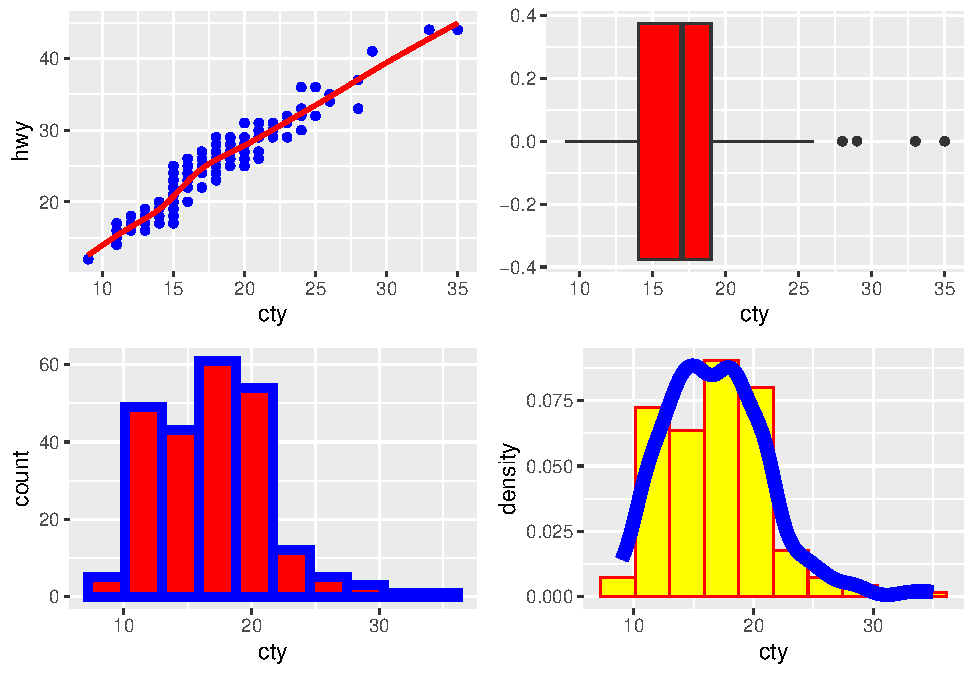
\includegraphics{02_ggplot2_files/figure-latex/unnamed-chunk-6-1.pdf}

\begin{Shaded}
\begin{Highlighting}[]
\CommentTok{\# patchwork}
\NormalTok{v1 }\SpecialCharTok{+}\NormalTok{ v2}
\end{Highlighting}
\end{Shaded}

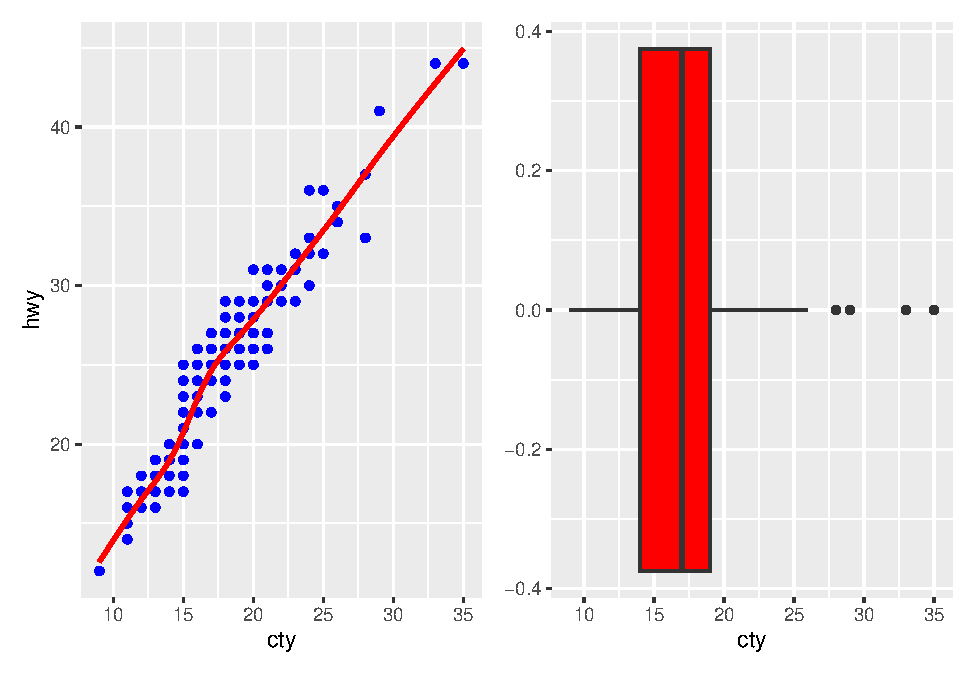
\includegraphics{02_ggplot2_files/figure-latex/unnamed-chunk-6-2.pdf}

\begin{Shaded}
\begin{Highlighting}[]
\NormalTok{v1 }\SpecialCharTok{|}\NormalTok{ v2}
\end{Highlighting}
\end{Shaded}

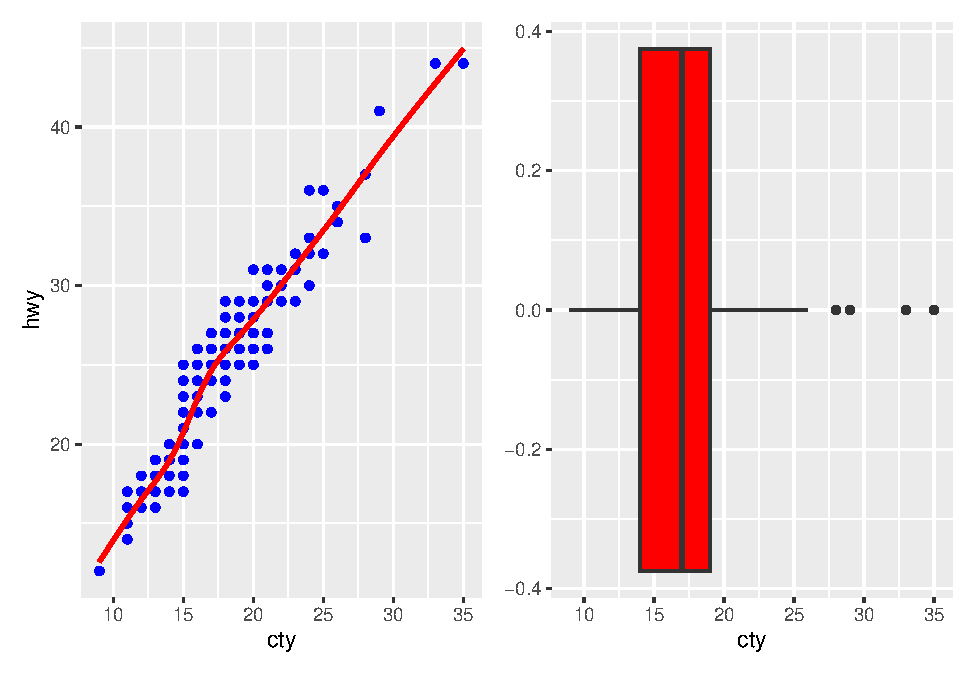
\includegraphics{02_ggplot2_files/figure-latex/unnamed-chunk-6-3.pdf}

\begin{Shaded}
\begin{Highlighting}[]
\NormalTok{v1 }\SpecialCharTok{/}\NormalTok{ v2}
\end{Highlighting}
\end{Shaded}

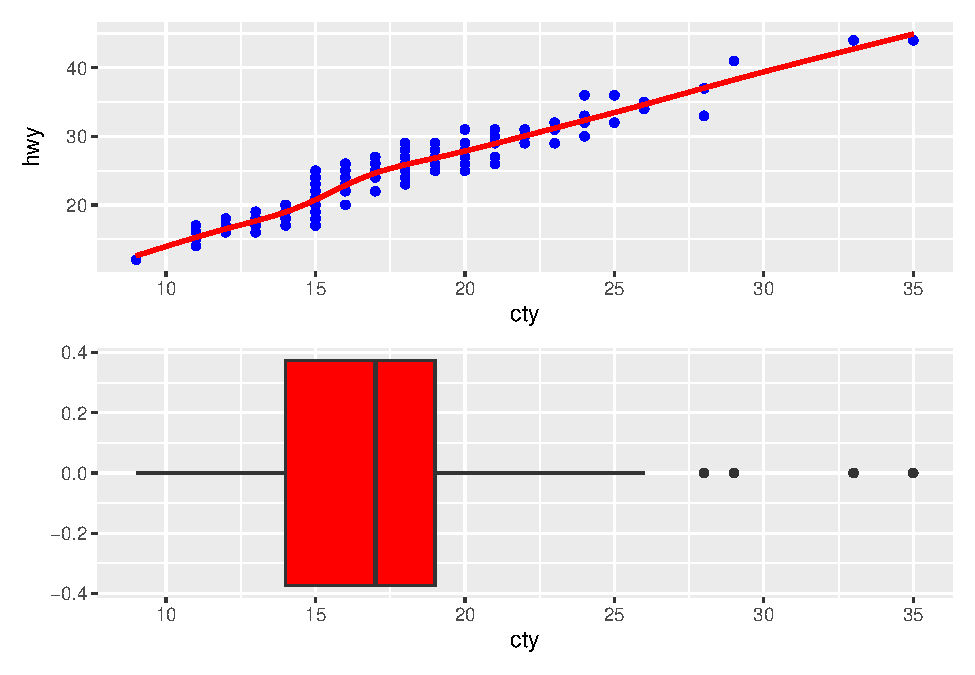
\includegraphics{02_ggplot2_files/figure-latex/unnamed-chunk-6-4.pdf}

\begin{Shaded}
\begin{Highlighting}[]
\NormalTok{v1 }\SpecialCharTok{+}\NormalTok{ v2 }\SpecialCharTok{+}\NormalTok{ v3}
\end{Highlighting}
\end{Shaded}

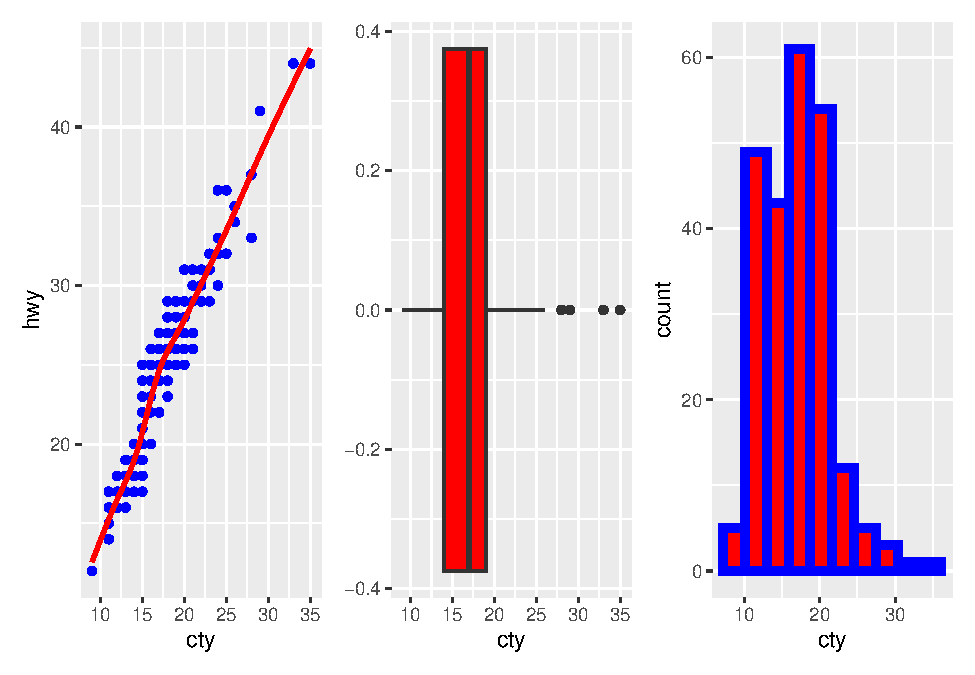
\includegraphics{02_ggplot2_files/figure-latex/unnamed-chunk-6-5.pdf}

\begin{Shaded}
\begin{Highlighting}[]
\NormalTok{v1 }\SpecialCharTok{+}\NormalTok{ (v2 }\SpecialCharTok{+}\NormalTok{ v3)}
\end{Highlighting}
\end{Shaded}

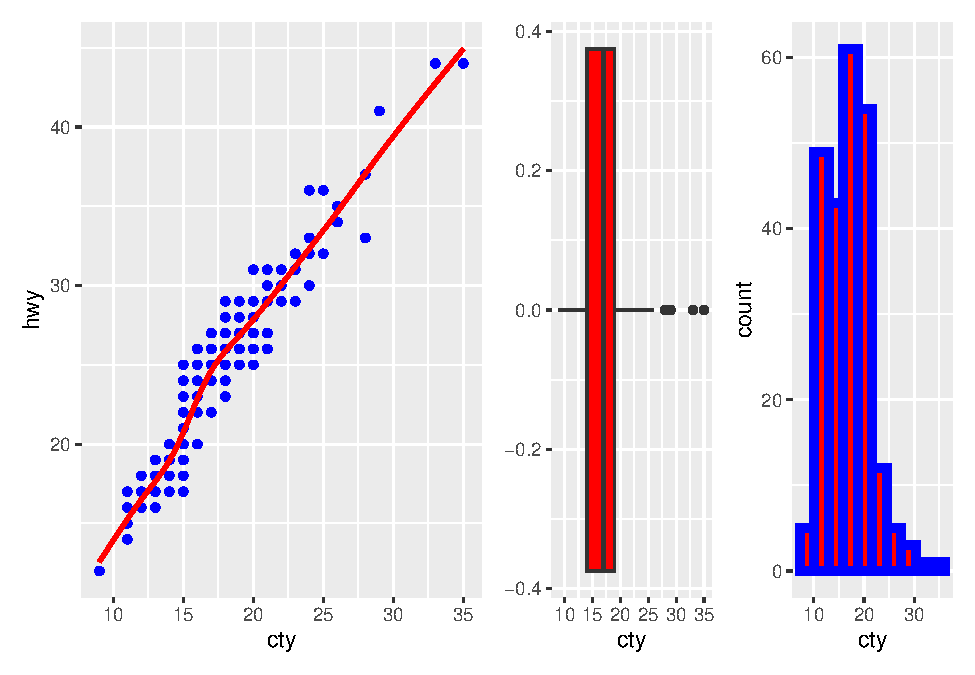
\includegraphics{02_ggplot2_files/figure-latex/unnamed-chunk-6-6.pdf}

\begin{Shaded}
\begin{Highlighting}[]
\NormalTok{v1 }\SpecialCharTok{|}\NormalTok{ (v2 }\SpecialCharTok{/}\NormalTok{ v3)}
\end{Highlighting}
\end{Shaded}

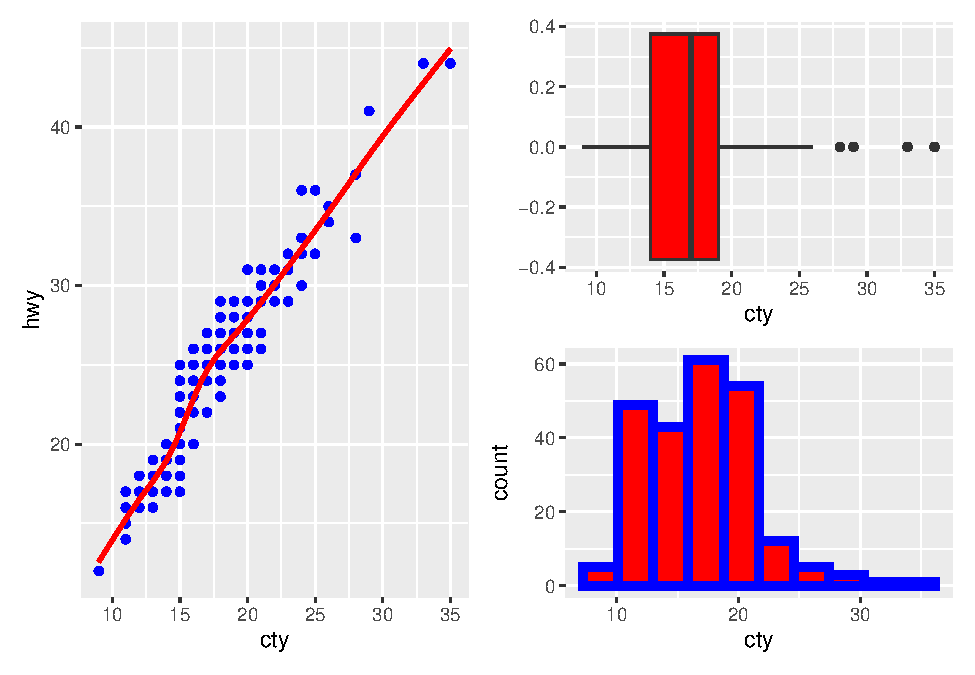
\includegraphics{02_ggplot2_files/figure-latex/unnamed-chunk-6-7.pdf}

\begin{Shaded}
\begin{Highlighting}[]
\NormalTok{v1 }\SpecialCharTok{/}\NormalTok{ (v2 }\SpecialCharTok{+}\NormalTok{ v3)}
\end{Highlighting}
\end{Shaded}

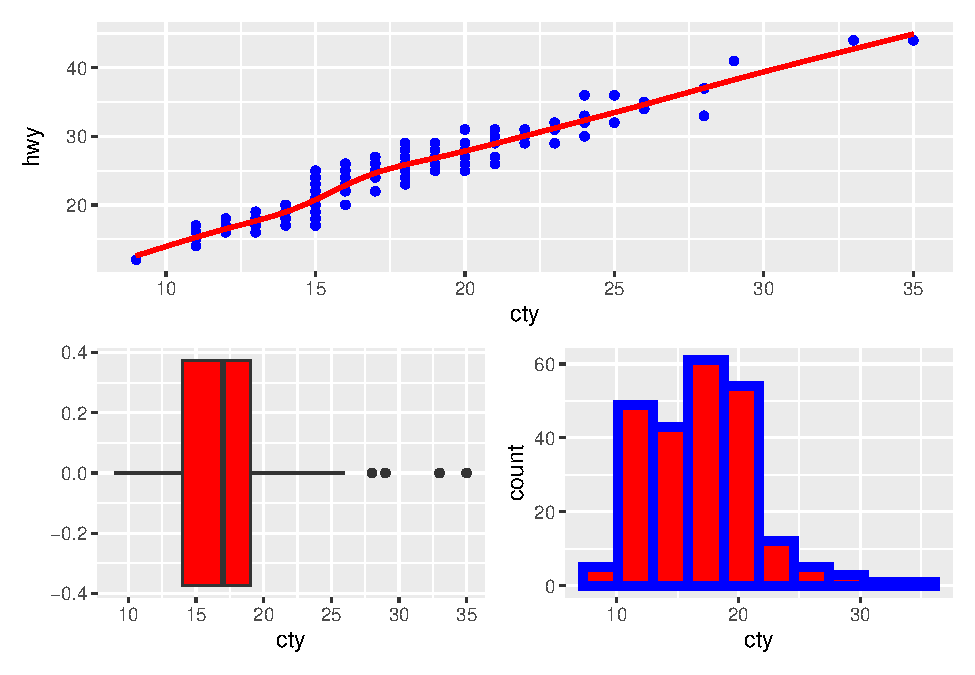
\includegraphics{02_ggplot2_files/figure-latex/unnamed-chunk-6-8.pdf}

\begin{Shaded}
\begin{Highlighting}[]
\NormalTok{v1 }\SpecialCharTok{+}\NormalTok{ v2 }\SpecialCharTok{+}\NormalTok{ v3 }\SpecialCharTok{+}\NormalTok{ v4 }
\end{Highlighting}
\end{Shaded}

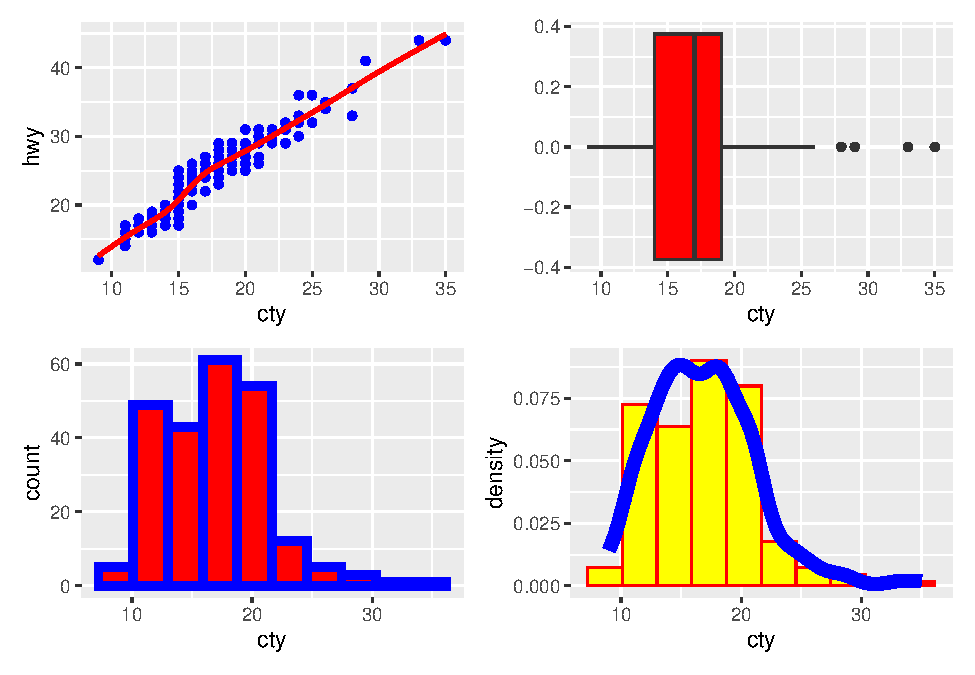
\includegraphics{02_ggplot2_files/figure-latex/unnamed-chunk-6-9.pdf}

\begin{Shaded}
\begin{Highlighting}[]
\NormalTok{v1}\SpecialCharTok{/}\NormalTok{(v2}\SpecialCharTok{+}\NormalTok{v3}\SpecialCharTok{+}\NormalTok{v4)}
\end{Highlighting}
\end{Shaded}

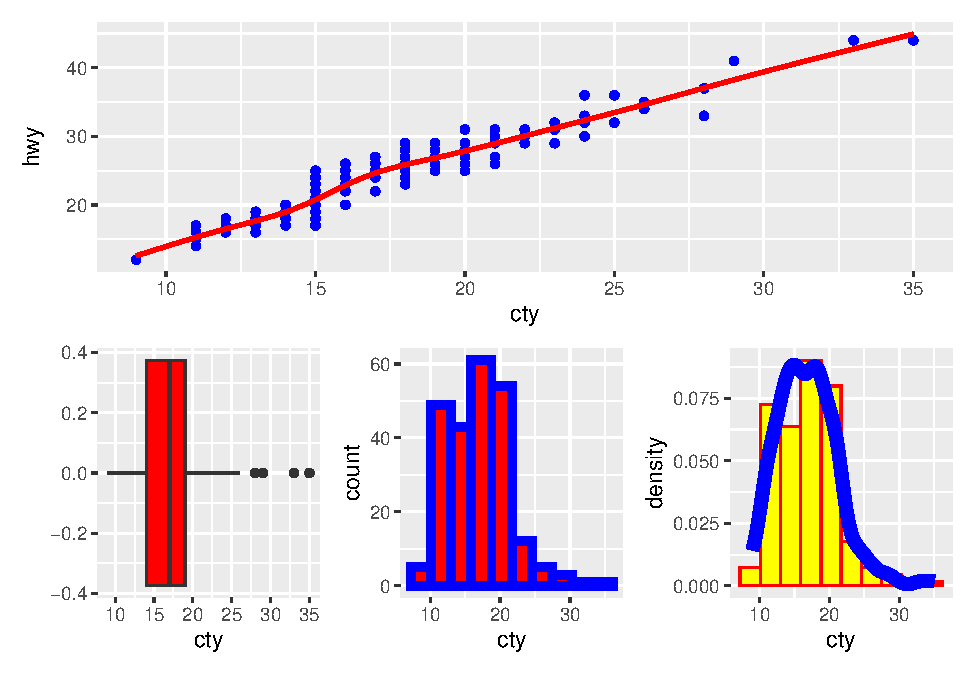
\includegraphics{02_ggplot2_files/figure-latex/unnamed-chunk-6-10.pdf}

\begin{Shaded}
\begin{Highlighting}[]
\NormalTok{v1  }\SpecialCharTok{+}\NormalTok{ (v2 }\SpecialCharTok{+}\NormalTok{ v3 }\SpecialCharTok{+}\NormalTok{ v4)}
\end{Highlighting}
\end{Shaded}

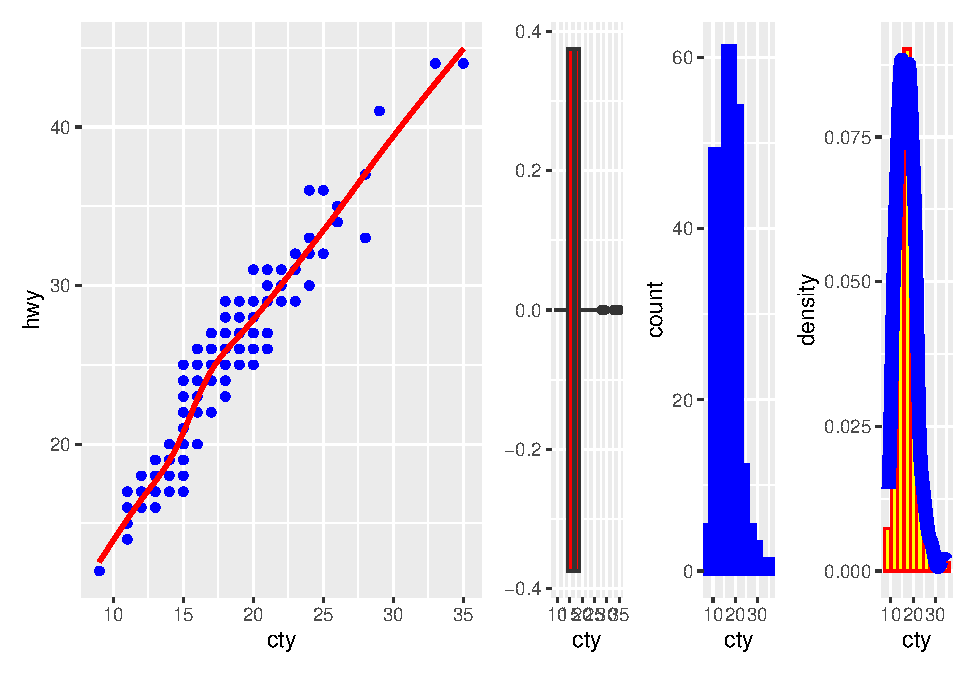
\includegraphics{02_ggplot2_files/figure-latex/unnamed-chunk-6-11.pdf}

\begin{Shaded}
\begin{Highlighting}[]
\NormalTok{v1  }\SpecialCharTok{+}\NormalTok{ v2 }\SpecialCharTok{+}\NormalTok{ (v3 }\SpecialCharTok{+}\NormalTok{ v4)}
\end{Highlighting}
\end{Shaded}

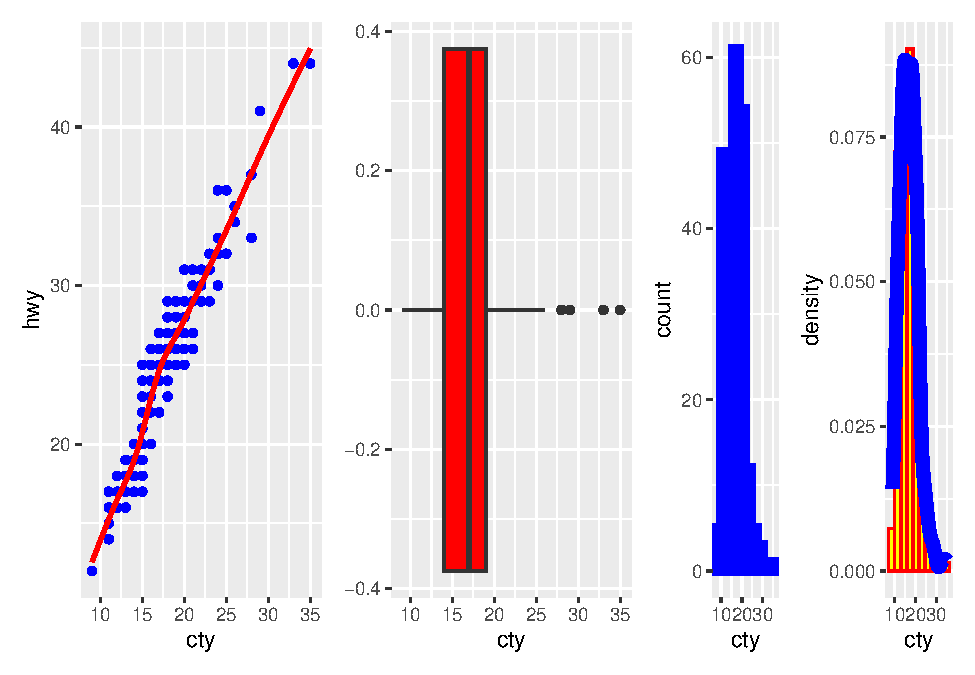
\includegraphics{02_ggplot2_files/figure-latex/unnamed-chunk-6-12.pdf}

\begin{Shaded}
\begin{Highlighting}[]
\NormalTok{(v1 }\SpecialCharTok{|}\NormalTok{ v2 }\SpecialCharTok{|}\NormalTok{ v3) }\SpecialCharTok{/}\NormalTok{ v4}
\end{Highlighting}
\end{Shaded}

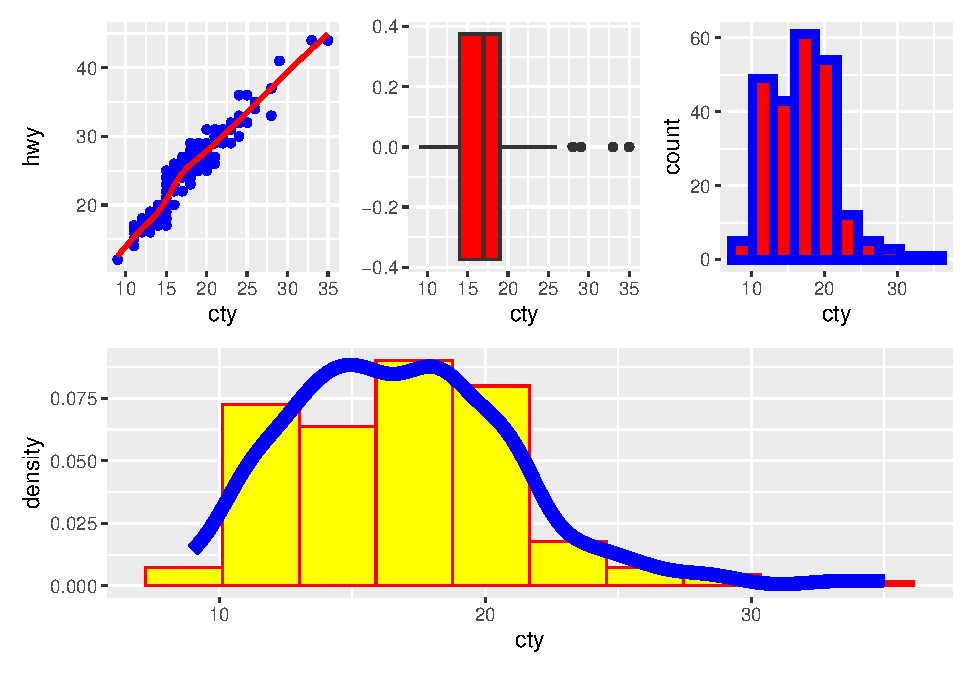
\includegraphics{02_ggplot2_files/figure-latex/unnamed-chunk-6-13.pdf}

\hypertarget{bar-col-density-density2d}{%
\section{bar, col, density, density2d}\label{bar-col-density-density2d}}

\begin{Shaded}
\begin{Highlighting}[]
\NormalTok{v5 }\OtherTok{\textless{}{-}} \FunctionTok{ggplot}\NormalTok{(dados , }\FunctionTok{aes}\NormalTok{(}\AttributeTok{x =}\NormalTok{ manufacturer)) }\SpecialCharTok{+} 
  \FunctionTok{geom\_bar}\NormalTok{()}\SpecialCharTok{+} 
  \FunctionTok{theme}\NormalTok{(}\AttributeTok{axis.text.x =} \FunctionTok{element\_text}\NormalTok{(}\AttributeTok{angle =} \DecValTok{45}\NormalTok{))}
\NormalTok{v5}
\end{Highlighting}
\end{Shaded}

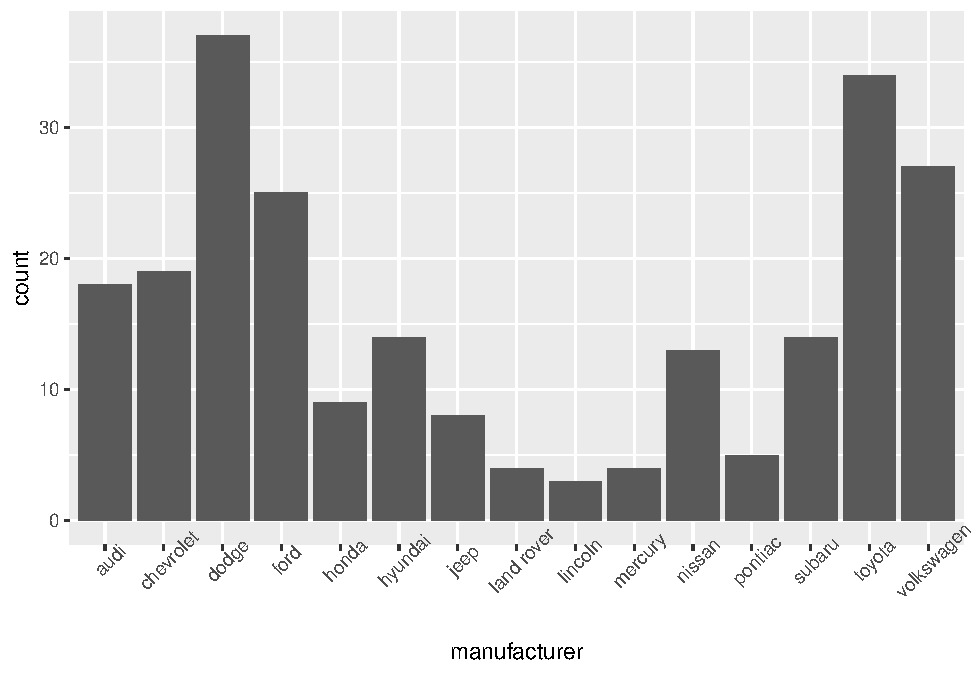
\includegraphics{02_ggplot2_files/figure-latex/unnamed-chunk-7-1.pdf}

\begin{Shaded}
\begin{Highlighting}[]
\CommentTok{\# Dúvidas no geom\_col}
\NormalTok{v6 }\OtherTok{\textless{}{-}} \FunctionTok{ggplot}\NormalTok{(dados , }\FunctionTok{aes}\NormalTok{(}\AttributeTok{x =}\NormalTok{ manufacturer, }\AttributeTok{y =}\NormalTok{ cty)) }\SpecialCharTok{+} 
  \FunctionTok{geom\_col}\NormalTok{()}\SpecialCharTok{+}
  \FunctionTok{theme}\NormalTok{(}\AttributeTok{axis.text.x =} \FunctionTok{element\_text}\NormalTok{(}\AttributeTok{angle =} \DecValTok{45}\NormalTok{))}
\NormalTok{v6}
\end{Highlighting}
\end{Shaded}

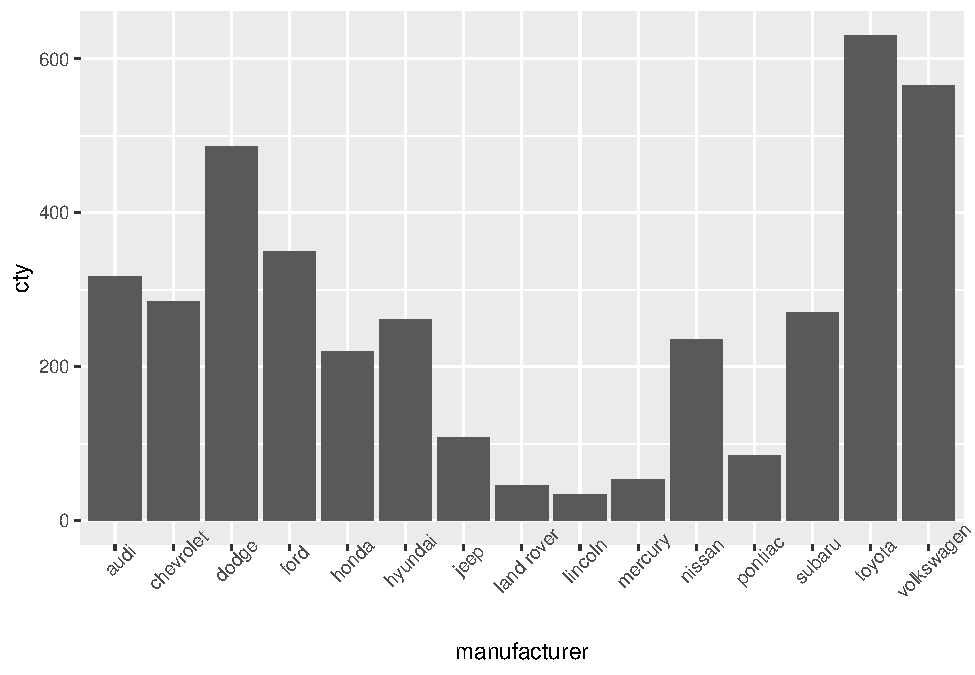
\includegraphics{02_ggplot2_files/figure-latex/unnamed-chunk-7-2.pdf}

\begin{Shaded}
\begin{Highlighting}[]
\NormalTok{dados }\SpecialCharTok{\%\textgreater{}\%} 
  \FunctionTok{select}\NormalTok{(manufacturer, cty) }\SpecialCharTok{\%\textgreater{}\%} 
  \FunctionTok{group\_by}\NormalTok{(manufacturer) }\SpecialCharTok{\%\textgreater{}\%} 
  \FunctionTok{summarise}\NormalTok{(}\AttributeTok{soma\_total\_cty =} \FunctionTok{sum}\NormalTok{(cty),}
            \AttributeTok{n =} \FunctionTok{n}\NormalTok{())}
\end{Highlighting}
\end{Shaded}

\begin{verbatim}
## # A tibble: 15 x 3
##    manufacturer soma_total_cty     n
##    <chr>                 <int> <int>
##  1 audi                    317    18
##  2 chevrolet               285    19
##  3 dodge                   486    37
##  4 ford                    350    25
##  5 honda                   220     9
##  6 hyundai                 261    14
##  7 jeep                    108     8
##  8 land rover               46     4
##  9 lincoln                  34     3
## 10 mercury                  53     4
## 11 nissan                  235    13
## 12 pontiac                  85     5
## 13 subaru                  270    14
## 14 toyota                  630    34
## 15 volkswagen              565    27
\end{verbatim}

\begin{Shaded}
\begin{Highlighting}[]
\CommentTok{\# dados \%\textgreater{}\% }
\CommentTok{\#   filter(manufacturer == "audi") \%\textgreater{}\% }
\CommentTok{\#   select(cty) \%\textgreater{}\% }
\CommentTok{\#   sum()}
\NormalTok{v7 }\OtherTok{\textless{}{-}} \FunctionTok{ggplot}\NormalTok{(dados , }\FunctionTok{aes}\NormalTok{(}\AttributeTok{x =}\NormalTok{ cty)) }\SpecialCharTok{+} 
  \FunctionTok{geom\_density}\NormalTok{()}
\NormalTok{v7}
\end{Highlighting}
\end{Shaded}

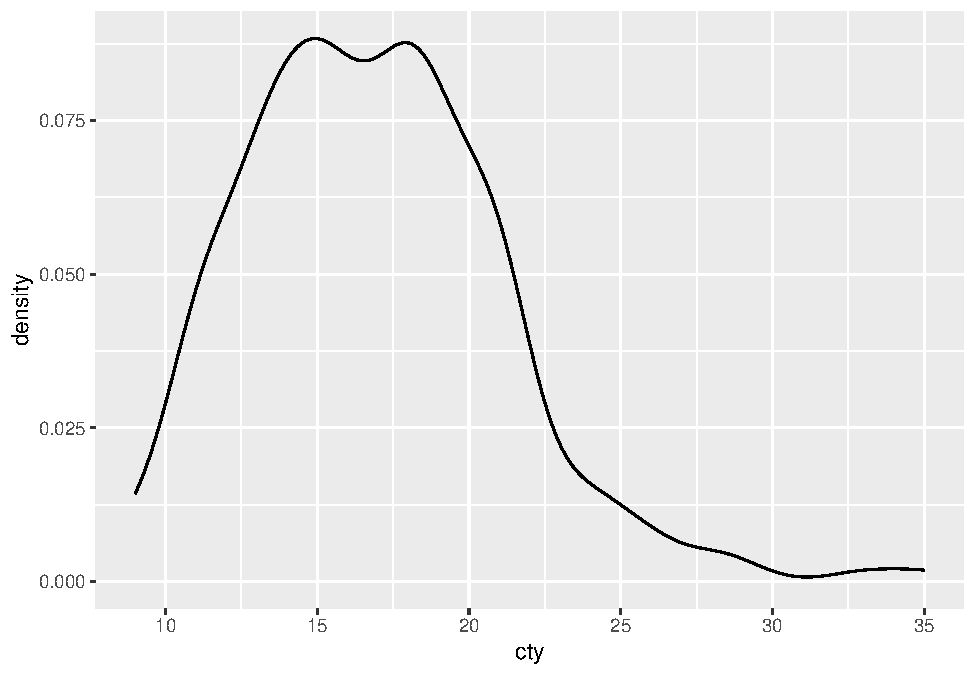
\includegraphics{02_ggplot2_files/figure-latex/unnamed-chunk-7-3.pdf}

\begin{Shaded}
\begin{Highlighting}[]
\NormalTok{v8 }\OtherTok{\textless{}{-}} \FunctionTok{ggplot}\NormalTok{(dados, }\FunctionTok{aes}\NormalTok{(}\AttributeTok{x =}\NormalTok{ cty, }\AttributeTok{y =}\NormalTok{ hwy)) }\SpecialCharTok{+} 
  \FunctionTok{geom\_density2d}\NormalTok{()}\SpecialCharTok{+}
  \FunctionTok{geom\_point}\NormalTok{(}\AttributeTok{colour =} \StringTok{"red"}\NormalTok{)}
\NormalTok{v8}
\end{Highlighting}
\end{Shaded}

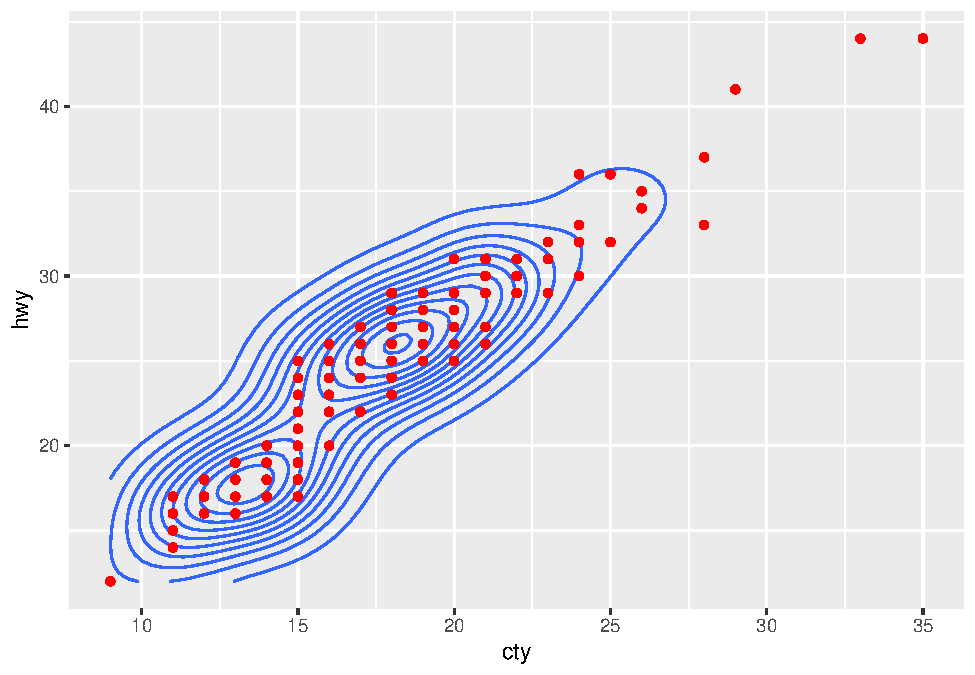
\includegraphics{02_ggplot2_files/figure-latex/unnamed-chunk-7-4.pdf}

\begin{Shaded}
\begin{Highlighting}[]
\NormalTok{(v5}\SpecialCharTok{+}\NormalTok{v6)}\SpecialCharTok{/}\NormalTok{ (v7 }\SpecialCharTok{+}\NormalTok{ v8)}
\end{Highlighting}
\end{Shaded}

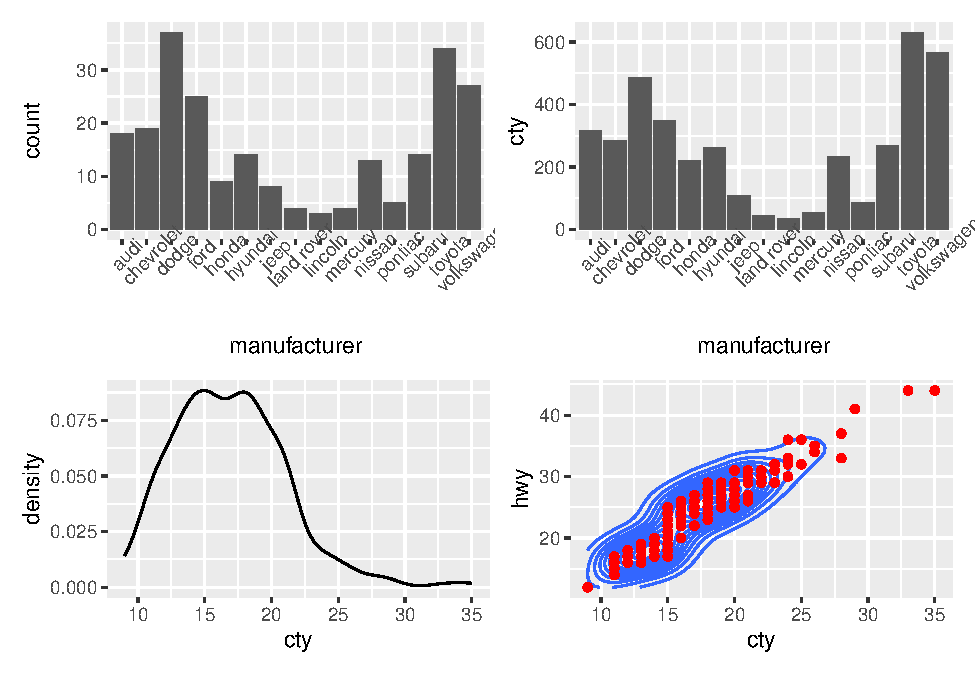
\includegraphics{02_ggplot2_files/figure-latex/unnamed-chunk-7-5.pdf}

\begin{Shaded}
\begin{Highlighting}[]
\CommentTok{\# Deixar pra depois...}
\NormalTok{ dados }\SpecialCharTok{\%\textgreater{}\%} 
    \FunctionTok{select}\NormalTok{(manufacturer, hwy, year) }\SpecialCharTok{\%\textgreater{}\%} 
    \FunctionTok{filter}\NormalTok{(manufacturer }\SpecialCharTok{==} \StringTok{"audi"}\NormalTok{, year }\SpecialCharTok{==} \StringTok{"1999"}\NormalTok{) }\SpecialCharTok{\%\textgreater{}\%} 
    \FunctionTok{summarise}\NormalTok{(}\AttributeTok{media =} \FunctionTok{max}\NormalTok{(hwy))}
\end{Highlighting}
\end{Shaded}

\begin{verbatim}
## # A tibble: 1 x 1
##   media
##   <int>
## 1    29
\end{verbatim}

\begin{Shaded}
\begin{Highlighting}[]
\CommentTok{\# plotly}
\FunctionTok{ggplotly}\NormalTok{(}
\FunctionTok{ggplot}\NormalTok{(dados, }\FunctionTok{aes}\NormalTok{(}\AttributeTok{x =}\NormalTok{ manufacturer, }\AttributeTok{y =}\NormalTok{ hwy, }\AttributeTok{fill =} \FunctionTok{factor}\NormalTok{(year))) }\SpecialCharTok{+} 
  \FunctionTok{geom\_col}\NormalTok{(}\AttributeTok{position =} \StringTok{"dodge"}\NormalTok{) }\SpecialCharTok{+} 
  \FunctionTok{labs}\NormalTok{(}\AttributeTok{fill =} \StringTok{"year"}\NormalTok{) }\SpecialCharTok{+}
  \FunctionTok{theme}\NormalTok{(}\AttributeTok{axis.text.x =} \FunctionTok{element\_text}\NormalTok{(}\AttributeTok{angle =} \DecValTok{45}\NormalTok{)))}

\NormalTok{dados }\SpecialCharTok{\%\textgreater{}\%} \FunctionTok{select}\NormalTok{(manufacturer, hwy, year) }\SpecialCharTok{\%\textgreater{}\%} 
  \FunctionTok{group\_by}\NormalTok{(manufacturer, year) }\SpecialCharTok{\%\textgreater{}\%} 
  \FunctionTok{summarise}\NormalTok{(}\AttributeTok{media =} \FunctionTok{mean}\NormalTok{(hwy))}
\end{Highlighting}
\end{Shaded}

\begin{Shaded}
\begin{Highlighting}[]
\CommentTok{\# Para pensar}

\NormalTok{(dados\_trat }\OtherTok{\textless{}{-}} \FunctionTok{data.frame}\NormalTok{(}\AttributeTok{tratamento =}\NormalTok{ LETTERS[}\DecValTok{1}\SpecialCharTok{:}\DecValTok{3}\NormalTok{], }
                         \AttributeTok{resposta =} \FunctionTok{c}\NormalTok{(}\FloatTok{2.3}\NormalTok{, }\FloatTok{1.9}\NormalTok{, }\FloatTok{3.2}\NormalTok{)))}
\end{Highlighting}
\end{Shaded}

\begin{verbatim}
##   tratamento resposta
## 1          A      2.3
## 2          B      1.9
## 3          C      3.2
\end{verbatim}

\begin{Shaded}
\begin{Highlighting}[]
\FunctionTok{ggplot}\NormalTok{(dados\_trat, }\FunctionTok{aes}\NormalTok{(tratamento, resposta)) }\SpecialCharTok{+}
  \FunctionTok{geom\_col}\NormalTok{(}\AttributeTok{fill =} \StringTok{"red"}\NormalTok{)}
\end{Highlighting}
\end{Shaded}

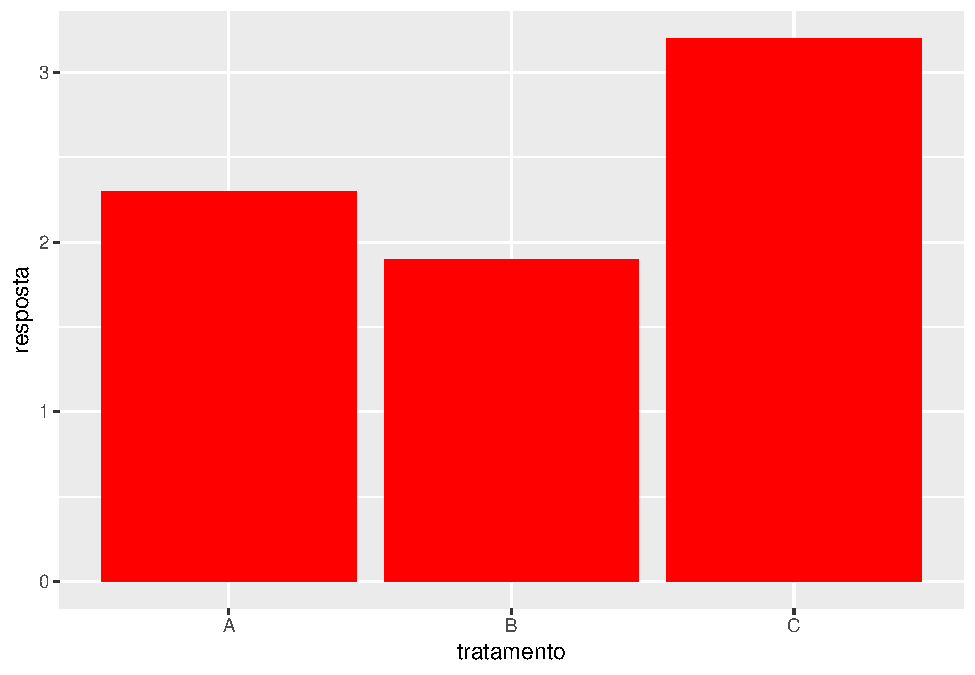
\includegraphics{02_ggplot2_files/figure-latex/unnamed-chunk-9-1.pdf}

\begin{Shaded}
\begin{Highlighting}[]
\CommentTok{\# Mais detalhes...}
\NormalTok{dados }\SpecialCharTok{\%\textgreater{}\%} \FunctionTok{select}\NormalTok{(manufacturer, hwy, year) }\SpecialCharTok{\%\textgreater{}\%} 
  \FunctionTok{group\_by}\NormalTok{(manufacturer, year) }\SpecialCharTok{\%\textgreater{}\%} 
  \FunctionTok{summarise}\NormalTok{(}\AttributeTok{media =} \FunctionTok{mean}\NormalTok{(hwy), }\AttributeTok{.groups =} \StringTok{"drop"}\NormalTok{) }\SpecialCharTok{\%\textgreater{}\%} 
  \FunctionTok{ggplot}\NormalTok{(}\FunctionTok{aes}\NormalTok{(}\AttributeTok{x =}\NormalTok{ manufacturer, }\AttributeTok{y =}\NormalTok{ media, }\AttributeTok{fill =} \FunctionTok{factor}\NormalTok{(year)))}\SpecialCharTok{+}
  \FunctionTok{geom\_col}\NormalTok{(}\AttributeTok{position =} \StringTok{"dodge"}\NormalTok{)}\SpecialCharTok{+}
  \FunctionTok{labs}\NormalTok{(}\AttributeTok{fill =} \StringTok{"year"}\NormalTok{) }\SpecialCharTok{+}
  \FunctionTok{theme}\NormalTok{(}\AttributeTok{axis.text.x =} \FunctionTok{element\_text}\NormalTok{(}\AttributeTok{angle =} \DecValTok{45}\NormalTok{))}
\end{Highlighting}
\end{Shaded}

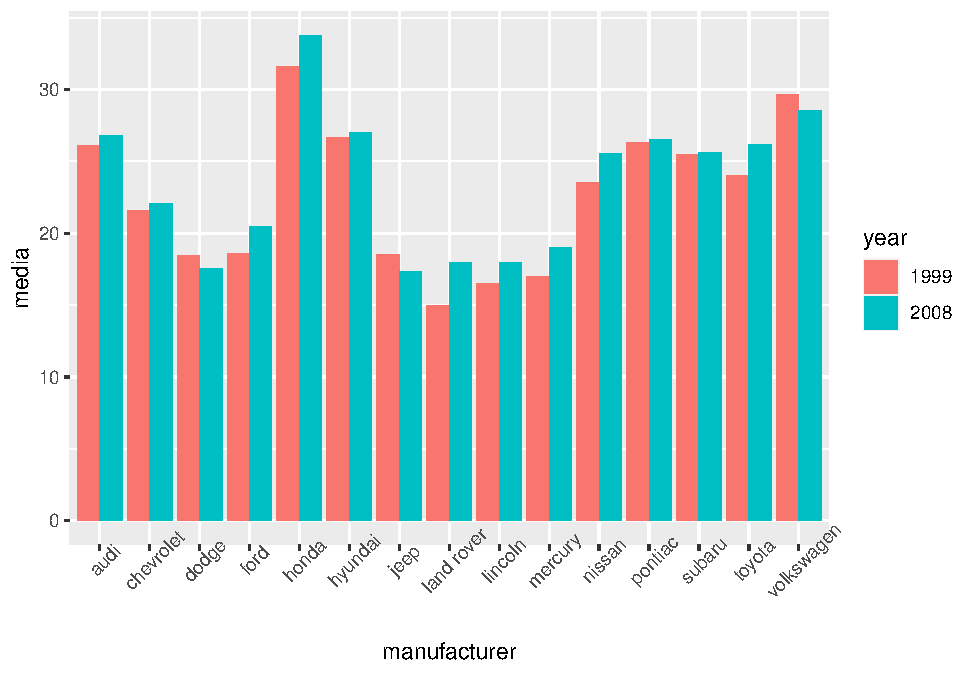
\includegraphics{02_ggplot2_files/figure-latex/unnamed-chunk-9-2.pdf}

\hypertarget{facet_grid-facet_wrap}{%
\section{facet\_grid, facet\_wrap}\label{facet_grid-facet_wrap}}

\begin{Shaded}
\begin{Highlighting}[]
\NormalTok{p1}\OtherTok{\textless{}{-}} \FunctionTok{ggplot}\NormalTok{(dados, }\FunctionTok{aes}\NormalTok{(}\AttributeTok{x =}\NormalTok{ cty, }\AttributeTok{y =}\NormalTok{ hwy)) }\SpecialCharTok{+}
  \FunctionTok{geom\_point}\NormalTok{()}
\NormalTok{p1}
\end{Highlighting}
\end{Shaded}

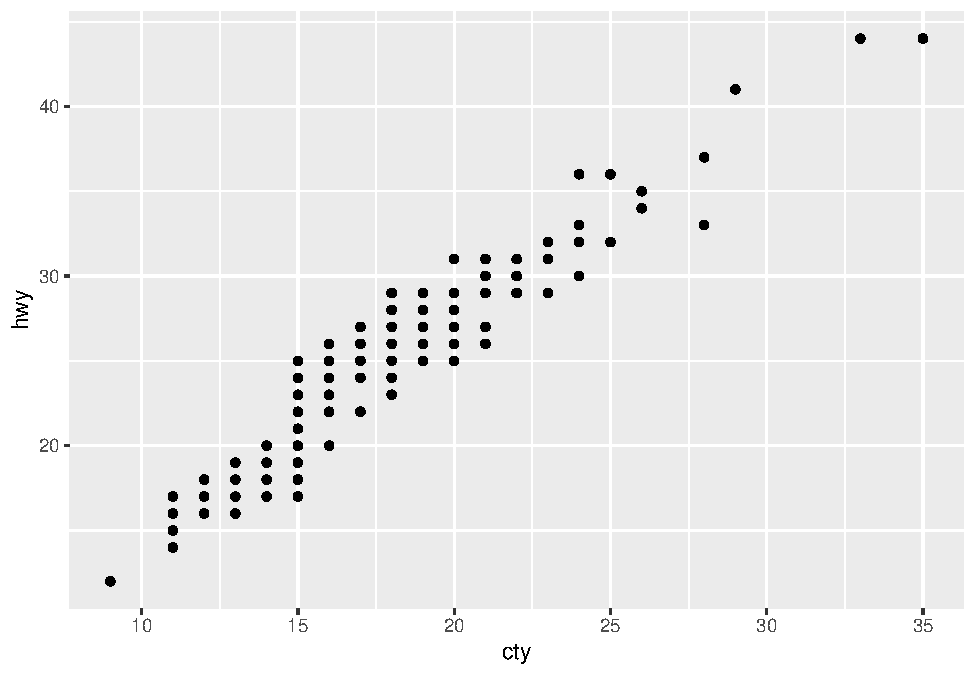
\includegraphics{02_ggplot2_files/figure-latex/unnamed-chunk-10-1.pdf}

\begin{Shaded}
\begin{Highlighting}[]
\NormalTok{p1 }\SpecialCharTok{+} \FunctionTok{facet\_grid}\NormalTok{(}\AttributeTok{rows =} \FunctionTok{vars}\NormalTok{(cyl))}
\end{Highlighting}
\end{Shaded}

\includegraphics{02_ggplot2_files/figure-latex/unnamed-chunk-10-2.pdf}

\begin{Shaded}
\begin{Highlighting}[]
\NormalTok{p1 }\SpecialCharTok{+} \FunctionTok{facet\_grid}\NormalTok{(}\AttributeTok{cols =} \FunctionTok{vars}\NormalTok{(cyl))}
\end{Highlighting}
\end{Shaded}

\includegraphics{02_ggplot2_files/figure-latex/unnamed-chunk-10-3.pdf}

\begin{Shaded}
\begin{Highlighting}[]
\NormalTok{p1 }\SpecialCharTok{+} \FunctionTok{facet\_grid}\NormalTok{(}\SpecialCharTok{\textasciitilde{}}\NormalTok{cyl)}
\end{Highlighting}
\end{Shaded}

\includegraphics{02_ggplot2_files/figure-latex/unnamed-chunk-10-4.pdf}

\begin{Shaded}
\begin{Highlighting}[]
\NormalTok{p1 }\SpecialCharTok{+} \FunctionTok{facet\_grid}\NormalTok{(}\AttributeTok{rows =} \FunctionTok{vars}\NormalTok{(year), }\AttributeTok{cols =}\FunctionTok{vars}\NormalTok{(cyl))}
\end{Highlighting}
\end{Shaded}

\includegraphics{02_ggplot2_files/figure-latex/unnamed-chunk-10-5.pdf}

\begin{Shaded}
\begin{Highlighting}[]
\NormalTok{p1 }\SpecialCharTok{+} \FunctionTok{facet\_grid}\NormalTok{(year}\SpecialCharTok{\textasciitilde{}}\NormalTok{cyl)}
\end{Highlighting}
\end{Shaded}

\includegraphics{02_ggplot2_files/figure-latex/unnamed-chunk-10-6.pdf}

\begin{Shaded}
\begin{Highlighting}[]
\NormalTok{p1 }\SpecialCharTok{+} \FunctionTok{facet\_wrap}\NormalTok{(year }\SpecialCharTok{\textasciitilde{}}\NormalTok{ cyl)}
\end{Highlighting}
\end{Shaded}

\includegraphics{02_ggplot2_files/figure-latex/unnamed-chunk-10-7.pdf}

\begin{Shaded}
\begin{Highlighting}[]
\NormalTok{p1 }\SpecialCharTok{+} \FunctionTok{facet\_wrap}\NormalTok{(cyl }\SpecialCharTok{\textasciitilde{}}\NormalTok{ year)}
\end{Highlighting}
\end{Shaded}

\includegraphics{02_ggplot2_files/figure-latex/unnamed-chunk-10-8.pdf}

\begin{Shaded}
\begin{Highlighting}[]
\NormalTok{p1 }\SpecialCharTok{+} \FunctionTok{facet\_wrap}\NormalTok{(}\SpecialCharTok{\textasciitilde{}}\NormalTok{cyl }\SpecialCharTok{+}\NormalTok{ year)}
\end{Highlighting}
\end{Shaded}

\includegraphics{02_ggplot2_files/figure-latex/unnamed-chunk-10-9.pdf}

\begin{Shaded}
\begin{Highlighting}[]
\NormalTok{p1 }\SpecialCharTok{+} \FunctionTok{facet\_wrap}\NormalTok{(}\SpecialCharTok{\textasciitilde{}}\NormalTok{year }\SpecialCharTok{+}\NormalTok{ cyl)}
\end{Highlighting}
\end{Shaded}

\includegraphics{02_ggplot2_files/figure-latex/unnamed-chunk-10-10.pdf}

\begin{Shaded}
\begin{Highlighting}[]
\NormalTok{p1 }\SpecialCharTok{+} \FunctionTok{facet\_wrap}\NormalTok{(year }\SpecialCharTok{\textasciitilde{}}\NormalTok{ cyl, }\AttributeTok{ncol =} \DecValTok{4}\NormalTok{)}
\end{Highlighting}
\end{Shaded}

\includegraphics{02_ggplot2_files/figure-latex/unnamed-chunk-10-11.pdf}

\begin{Shaded}
\begin{Highlighting}[]
\NormalTok{p1 }\SpecialCharTok{+} \FunctionTok{facet\_wrap}\NormalTok{(cyl }\SpecialCharTok{\textasciitilde{}}\NormalTok{ year, }\AttributeTok{ncol =} \DecValTok{4}\NormalTok{)}
\end{Highlighting}
\end{Shaded}

\includegraphics{02_ggplot2_files/figure-latex/unnamed-chunk-10-12.pdf}

\hypertarget{stat_function}{%
\section{stat\_function}\label{stat_function}}

\begin{Shaded}
\begin{Highlighting}[]
\NormalTok{a}\OtherTok{\textless{}{-}} \SpecialCharTok{{-}}\DecValTok{3} \CommentTok{\# média}
\NormalTok{b}\OtherTok{\textless{}{-}} \DecValTok{4}  \CommentTok{\# desv. padrão}
\FunctionTok{ggplot}\NormalTok{(}\FunctionTok{data.frame}\NormalTok{(}\AttributeTok{x =} \FunctionTok{c}\NormalTok{(a }\SpecialCharTok{{-}} \DecValTok{3}\SpecialCharTok{*}\NormalTok{b, a }\SpecialCharTok{+} \DecValTok{3}\SpecialCharTok{*}\NormalTok{b)), }\FunctionTok{aes}\NormalTok{(x)) }\SpecialCharTok{+} 
  \FunctionTok{stat\_function}\NormalTok{(}\AttributeTok{fun =}\NormalTok{ dnorm, }\AttributeTok{args =} \FunctionTok{list}\NormalTok{(}\AttributeTok{mean =}\NormalTok{ a, }\AttributeTok{sd =}\NormalTok{ b))}\SpecialCharTok{+}
  \FunctionTok{geom\_vline}\NormalTok{(}\AttributeTok{xintercept =} \FunctionTok{c}\NormalTok{(a }\SpecialCharTok{{-}} \DecValTok{3}\SpecialCharTok{*}\NormalTok{b, a, a }\SpecialCharTok{+} \DecValTok{3}\SpecialCharTok{*}\NormalTok{b), }\AttributeTok{col =} \StringTok{"red"}\NormalTok{, }\AttributeTok{lty =} \DecValTok{2}\NormalTok{)}\SpecialCharTok{+}
  \FunctionTok{theme\_minimal}\NormalTok{()}
\end{Highlighting}
\end{Shaded}

\includegraphics{02_ggplot2_files/figure-latex/unnamed-chunk-11-1.pdf}

\hypertarget{stat_summary}{%
\section{stat\_summary}\label{stat_summary}}

\begin{Shaded}
\begin{Highlighting}[]
\FunctionTok{ggplot}\NormalTok{(dados, }\FunctionTok{aes}\NormalTok{(}\AttributeTok{x =}\NormalTok{ manufacturer, }\AttributeTok{y =}\NormalTok{ hwy)) }\SpecialCharTok{+} 
  \FunctionTok{geom\_boxplot}\NormalTok{()}\SpecialCharTok{+}
  \FunctionTok{geom\_point}\NormalTok{(}\AttributeTok{col =} \StringTok{"red"}\NormalTok{, }\AttributeTok{size=}\FloatTok{0.8}\NormalTok{)}\SpecialCharTok{+}
  \FunctionTok{stat\_summary}\NormalTok{(}\AttributeTok{fun =}\NormalTok{ mean, }\AttributeTok{col =} \StringTok{"blue"}\NormalTok{)}\SpecialCharTok{+}
  \FunctionTok{theme\_minimal}\NormalTok{()}\SpecialCharTok{+}
  \FunctionTok{theme}\NormalTok{(}\AttributeTok{axis.text.x =} \FunctionTok{element\_text}\NormalTok{(}\AttributeTok{angle =} \DecValTok{45}\NormalTok{))}
\end{Highlighting}
\end{Shaded}

\includegraphics{02_ggplot2_files/figure-latex/unnamed-chunk-12-1.pdf}

\hypertarget{theme_}{%
\section{theme\_*()}\label{theme_}}

\begin{Shaded}
\begin{Highlighting}[]
\NormalTok{a1}\OtherTok{\textless{}{-}}\NormalTok{ p1 }\SpecialCharTok{+} \FunctionTok{theme\_bw}\NormalTok{() }\SpecialCharTok{+} \FunctionTok{labs}\NormalTok{(}\AttributeTok{title =} \StringTok{"theme\_bw()"}\NormalTok{)}
\NormalTok{a2}\OtherTok{\textless{}{-}}\NormalTok{ p1 }\SpecialCharTok{+} \FunctionTok{theme\_classic}\NormalTok{() }\SpecialCharTok{+} \FunctionTok{labs}\NormalTok{(}\AttributeTok{title =} \StringTok{"theme\_classic()"}\NormalTok{)}
\NormalTok{a3}\OtherTok{\textless{}{-}}\NormalTok{ p1 }\SpecialCharTok{+} \FunctionTok{theme\_light}\NormalTok{() }\SpecialCharTok{+} \FunctionTok{labs}\NormalTok{(}\AttributeTok{title =} \StringTok{"theme\_light()"}\NormalTok{)}
\NormalTok{a4}\OtherTok{\textless{}{-}}\NormalTok{ p1 }\SpecialCharTok{+} \FunctionTok{theme\_minimal}\NormalTok{() }\SpecialCharTok{+} \FunctionTok{labs}\NormalTok{(}\AttributeTok{title =} \StringTok{"theme\_minimal()"}\NormalTok{)}

\NormalTok{a1 }\SpecialCharTok{+}\NormalTok{ a2 }\SpecialCharTok{+}\NormalTok{ a3 }\SpecialCharTok{+}\NormalTok{ a4}
\end{Highlighting}
\end{Shaded}

\includegraphics{02_ggplot2_files/figure-latex/unnamed-chunk-13-1.pdf}

\hypertarget{gruxe1fico-de-perfis-spaguetti-plot}{%
\section{Gráfico de perfis (Spaguetti plot)}\label{gruxe1fico-de-perfis-spaguetti-plot}}

\begin{Shaded}
\begin{Highlighting}[]
\FunctionTok{glimpse}\NormalTok{(Orange)}
\end{Highlighting}
\end{Shaded}

\begin{verbatim}
## Rows: 35
## Columns: 3
## $ Tree          <ord> 1, 1, 1, 1, 1, 1, 1, 2, 2, 2, 2, 2, 2, 2, 3, 3, 3, 3, 3,~
## $ age           <dbl> 118, 484, 664, 1004, 1231, 1372, 1582, 118, 484, 664, 10~
## $ circumference <dbl> 30, 58, 87, 115, 120, 142, 145, 33, 69, 111, 156, 172, 2~
\end{verbatim}

\begin{Shaded}
\begin{Highlighting}[]
\FunctionTok{ggplot}\NormalTok{(Orange, }\FunctionTok{aes}\NormalTok{(}\AttributeTok{x =}\NormalTok{ age, }\AttributeTok{y =}\NormalTok{ circumference, }\AttributeTok{group =}\NormalTok{ Tree, }
                   \AttributeTok{col =}\NormalTok{ Tree)) }\SpecialCharTok{+}
  \FunctionTok{geom\_line}\NormalTok{()}\SpecialCharTok{+}
  \FunctionTok{stat\_summary}\NormalTok{(}\FunctionTok{aes}\NormalTok{(}\AttributeTok{group =} \DecValTok{1}\NormalTok{), }\AttributeTok{fun =}\NormalTok{ mean, }\AttributeTok{col =} \StringTok{"red"}\NormalTok{, }
               \AttributeTok{geom =} \StringTok{"line"}\NormalTok{, }\AttributeTok{size =} \DecValTok{1}\NormalTok{, }\AttributeTok{show.legend =} \ConstantTok{FALSE}\NormalTok{,}
               \AttributeTok{linetype =} \DecValTok{2}\NormalTok{)}\SpecialCharTok{+}
  \FunctionTok{xlim}\NormalTok{(}\DecValTok{0}\NormalTok{, }\DecValTok{1600}\NormalTok{)}\SpecialCharTok{+}
  \FunctionTok{theme\_minimal}\NormalTok{()}
\end{Highlighting}
\end{Shaded}

\includegraphics{02_ggplot2_files/figure-latex/unnamed-chunk-14-1.pdf}

\begin{Shaded}
\begin{Highlighting}[]
\FunctionTok{ggplot}\NormalTok{(Orange, }\FunctionTok{aes}\NormalTok{(}\AttributeTok{x =}\NormalTok{ age, }\AttributeTok{y =}\NormalTok{ circumference, }\AttributeTok{group =}\NormalTok{ Tree)) }\SpecialCharTok{+}
  \FunctionTok{geom\_line}\NormalTok{()}\SpecialCharTok{+}
  \FunctionTok{xlim}\NormalTok{(}\DecValTok{0}\NormalTok{, }\DecValTok{1600}\NormalTok{)}\SpecialCharTok{+}
  \FunctionTok{facet\_wrap}\NormalTok{(}\SpecialCharTok{\textasciitilde{}}\NormalTok{Tree)}\SpecialCharTok{+}
  \FunctionTok{theme\_minimal}\NormalTok{()}\SpecialCharTok{+}
  \FunctionTok{theme}\NormalTok{(}\AttributeTok{legend.position =} \StringTok{"none"}\NormalTok{)}
\end{Highlighting}
\end{Shaded}

\includegraphics{02_ggplot2_files/figure-latex/unnamed-chunk-14-2.pdf}

\hypertarget{plotly}{%
\section{plotly}\label{plotly}}

\href{https://cran.r-project.org/web/packages/plotly/index.html}{plotly cran}

\href{https://plotly-r.com/}{Interactive web-based data visualization with R, plotly, and shiny}

\href{https://plotly.com/r/}{Plotly R Open Source Graphing Library}

\begin{Shaded}
\begin{Highlighting}[]
\FunctionTok{ggplotly}\NormalTok{(v1)}
\FunctionTok{ggplotly}\NormalTok{(v2)}
\FunctionTok{ggplotly}\NormalTok{(v4)}
\FunctionTok{ggplotly}\NormalTok{(v5)}
\end{Highlighting}
\end{Shaded}

\hypertarget{esquisse}{%
\section{esquisse}\label{esquisse}}

Alguns links de interesse

\href{https://cran.r-project.org/web/packages/esquisse/vignettes/get-started.html}{esquisse}

\href{https://cran.r-project.org/web/packages/esquisse/vignettes/shiny-usage.html}{esquisse + shiny}

\begin{Shaded}
\begin{Highlighting}[]
\FunctionTok{esquisser}\NormalTok{(dados)}
\end{Highlighting}
\end{Shaded}

\hypertarget{exemplo-esquisse}{%
\section{Exemplo esquisse}\label{exemplo-esquisse}}

\begin{Shaded}
\begin{Highlighting}[]
\FunctionTok{ggplot}\NormalTok{(dados) }\SpecialCharTok{+}
  \FunctionTok{aes}\NormalTok{(}\AttributeTok{x =}\NormalTok{ displ, }\AttributeTok{y =}\NormalTok{ hwy, }\AttributeTok{colour =}\NormalTok{ drv) }\SpecialCharTok{+}
  \FunctionTok{geom\_point}\NormalTok{(}\AttributeTok{shape =} \StringTok{"circle"}\NormalTok{, }\AttributeTok{size =} \FloatTok{1.85}\NormalTok{) }\SpecialCharTok{+}
  \FunctionTok{scale\_color\_hue}\NormalTok{(}\AttributeTok{direction =} \DecValTok{1}\NormalTok{) }\SpecialCharTok{+}
  \FunctionTok{theme\_minimal}\NormalTok{() }\SpecialCharTok{+}
  \FunctionTok{theme}\NormalTok{(}\AttributeTok{legend.position =} \StringTok{"top"}\NormalTok{)}
\end{Highlighting}
\end{Shaded}

\includegraphics{02_ggplot2_files/figure-latex/unnamed-chunk-17-1.pdf}

\begin{Shaded}
\begin{Highlighting}[]
\FunctionTok{ggplot}\NormalTok{(dados) }\SpecialCharTok{+}
  \FunctionTok{aes}\NormalTok{(}\AttributeTok{x =}\NormalTok{ displ, }\AttributeTok{y =}\NormalTok{ cty, }\AttributeTok{colour =}\NormalTok{ class, }\AttributeTok{size =}\NormalTok{ cty) }\SpecialCharTok{+}
  \FunctionTok{geom\_point}\NormalTok{(}\AttributeTok{shape =} \StringTok{"circle"}\NormalTok{) }\SpecialCharTok{+}
  \FunctionTok{scale\_color\_hue}\NormalTok{(}\AttributeTok{direction =} \DecValTok{1}\NormalTok{) }\SpecialCharTok{+}
  \FunctionTok{theme}\NormalTok{(}\AttributeTok{legend.position =} \StringTok{"top"}\NormalTok{) }\SpecialCharTok{+}
  \FunctionTok{facet\_wrap}\NormalTok{(}\FunctionTok{vars}\NormalTok{(drv))}
\end{Highlighting}
\end{Shaded}

\includegraphics{02_ggplot2_files/figure-latex/unnamed-chunk-18-1.pdf}

\hypertarget{purrr}{%
\chapter{purrr}\label{purrr}}

\begin{Shaded}
\begin{Highlighting}[]
\FunctionTok{library}\NormalTok{(tidyverse)}
\FunctionTok{ls}\NormalTok{(}\StringTok{"package:purrr"}\NormalTok{)}
\end{Highlighting}
\end{Shaded}

\begin{verbatim}
##   [1] "%@%"                 "%||%"                "%>%"                
##   [4] "accumulate"          "accumulate_right"    "accumulate2"        
##   [7] "array_branch"        "array_tree"          "as_mapper"          
##  [10] "as_vector"           "assign_in"           "at_depth"           
##  [13] "attr_getter"         "auto_browse"         "chuck"              
##  [16] "compact"             "compose"             "cross"              
##  [19] "cross_d"             "cross_df"            "cross_n"            
##  [22] "cross2"              "cross3"              "detect"             
##  [25] "detect_index"        "discard"             "discard_at"         
##  [28] "done"                "every"               "exec"               
##  [31] "flatten"             "flatten_chr"         "flatten_dbl"        
##  [34] "flatten_df"          "flatten_dfc"         "flatten_dfr"        
##  [37] "flatten_int"         "flatten_lgl"         "flatten_raw"        
##  [40] "has_element"         "head_while"          "imap"               
##  [43] "imap_chr"            "imap_dbl"            "imap_dfc"           
##  [46] "imap_dfr"            "imap_int"            "imap_lgl"           
##  [49] "imap_raw"            "imodify"             "insistently"        
##  [52] "invoke"              "invoke_map"          "invoke_map_chr"     
##  [55] "invoke_map_dbl"      "invoke_map_df"       "invoke_map_dfc"     
##  [58] "invoke_map_dfr"      "invoke_map_int"      "invoke_map_lgl"     
##  [61] "invoke_map_raw"      "is_atomic"           "is_bare_atomic"     
##  [64] "is_bare_character"   "is_bare_double"      "is_bare_integer"    
##  [67] "is_bare_list"        "is_bare_logical"     "is_bare_numeric"    
##  [70] "is_bare_vector"      "is_character"        "is_double"          
##  [73] "is_empty"            "is_formula"          "is_function"        
##  [76] "is_integer"          "is_list"             "is_logical"         
##  [79] "is_null"             "is_rate"             "is_scalar_atomic"   
##  [82] "is_scalar_character" "is_scalar_double"    "is_scalar_integer"  
##  [85] "is_scalar_list"      "is_scalar_logical"   "is_scalar_vector"   
##  [88] "is_vector"           "iwalk"               "keep"               
##  [91] "keep_at"             "lift"                "lift_dl"            
##  [94] "lift_dv"             "lift_ld"             "lift_lv"            
##  [97] "lift_vd"             "lift_vl"             "list_along"         
## [100] "list_assign"         "list_c"              "list_cbind"         
## [103] "list_flatten"        "list_merge"          "list_modify"        
## [106] "list_rbind"          "list_simplify"       "list_transpose"     
## [109] "lmap"                "lmap_at"             "lmap_if"            
## [112] "map"                 "map_at"              "map_chr"            
## [115] "map_dbl"             "map_depth"           "map_df"             
## [118] "map_dfc"             "map_dfr"             "map_if"             
## [121] "map_int"             "map_lgl"             "map_raw"            
## [124] "map_vec"             "map2"                "map2_chr"           
## [127] "map2_dbl"            "map2_df"             "map2_dfc"           
## [130] "map2_dfr"            "map2_int"            "map2_lgl"           
## [133] "map2_raw"            "map2_vec"            "modify"             
## [136] "modify_at"           "modify_depth"        "modify_if"          
## [139] "modify_in"           "modify_tree"         "modify2"            
## [142] "negate"              "none"                "partial"            
## [145] "pluck"               "pluck_depth"         "pluck_exists"       
## [148] "pluck<-"             "pmap"                "pmap_chr"           
## [151] "pmap_dbl"            "pmap_df"             "pmap_dfc"           
## [154] "pmap_dfr"            "pmap_int"            "pmap_lgl"           
## [157] "pmap_raw"            "pmap_vec"            "possibly"           
## [160] "prepend"             "pwalk"               "quietly"            
## [163] "rate_backoff"        "rate_delay"          "rate_reset"         
## [166] "rate_sleep"          "rbernoulli"          "rdunif"             
## [169] "reduce"              "reduce_right"        "reduce2"            
## [172] "reduce2_right"       "rep_along"           "rerun"              
## [175] "safely"              "set_names"           "simplify"           
## [178] "simplify_all"        "slowly"              "some"               
## [181] "splice"              "tail_while"          "transpose"          
## [184] "update_list"         "vec_depth"           "walk"               
## [187] "walk2"               "when"                "zap"
\end{verbatim}

\hypertarget{map-functions}{%
\section{map functions}\label{map-functions}}

\begin{Shaded}
\begin{Highlighting}[]
\FunctionTok{example}\NormalTok{(}\StringTok{"map"}\NormalTok{)}
\end{Highlighting}
\end{Shaded}

\begin{verbatim}
## 
## map> # Compute normal distributions from an atomic vector
## map> 1:10 |>
## map+   map(rnorm, n = 10)
## [[1]]
##  [1] -0.21922348  0.61996465  1.29024877  0.11019642  0.59216413  0.87487471
##  [7]  0.39567527 -1.02818925 -0.81626024 -0.02669643
## 
## [[2]]
##  [1] 5.7748559 1.4410355 2.8421403 0.6115358 1.2729774 1.6114799 0.7816303
##  [8] 2.7443002 0.5157748 1.7379449
## 
## [[3]]
##  [1] 1.7785115 2.5023306 3.2356692 5.5216912 2.5630065 2.4648148 3.4178825
##  [8] 3.1202642 3.9779527 0.9282494
## 
## [[4]]
##  [1] 4.857196 3.571092 2.367683 3.389621 4.905757 4.102200 4.032000 3.443664
##  [9] 5.395998 4.641652
## 
## [[5]]
##  [1] 4.398464 6.080639 4.873609 4.843892 4.047706 4.245536 4.657401 3.671805
##  [9] 6.436675 3.743995
## 
## [[6]]
##  [1] 5.642601 5.902677 3.763949 6.788100 5.421124 8.629236 5.842409 5.309218
##  [9] 5.328469 5.649454
## 
## [[7]]
##  [1] 7.036166 6.369926 7.137499 6.989909 6.494763 8.151830 7.674627 7.274734
##  [9] 6.740540 6.973178
## 
## [[8]]
##  [1]  8.566392 10.646892  6.802248  8.860256  8.211045  6.536649  8.282630
##  [8]  8.011455  8.468509  7.119174
## 
## [[9]]
##  [1]  9.513433  9.958892 10.836989  9.675665  6.940989  9.308194 10.965672
##  [8]  9.068537  9.914014  8.871290
## 
## [[10]]
##  [1]  9.651390 10.108473  9.055043 10.582112  9.444427  9.998619  9.896081
##  [8] 10.241184  8.666145  9.672320
## 
## 
## map> # You can also use an anonymous function
## map> 1:10 |>
## map+   map(\(x) rnorm(10, x))
## [[1]]
##  [1]  0.8673994  1.7287065 -0.2481662 -1.1399910  1.6306988 -1.6557005
##  [7]  1.6206918  0.2477373  1.8680921  0.2386029
## 
## [[2]]
##  [1] 1.7421001 2.3557942 1.1523195 0.2790364 2.7476298 0.8111794 0.1694989
##  [8] 2.5691697 0.7063602 3.2158305
## 
## [[3]]
##  [1] 2.8730810 4.6178702 2.7328835 2.1959393 3.2452071 1.7167346 2.5633084
##  [8] 1.7339964 0.6740952 2.2906973
## 
## [[4]]
##  [1] 3.671998 3.479038 3.893398 4.631399 4.361525 2.408883 1.889459 3.219626
##  [9] 4.511175 2.397565
## 
## [[5]]
##  [1] 3.625986 4.499937 3.858146 4.846787 5.267548 4.840228 5.786236 5.374074
##  [9] 6.073319 4.707545
## 
## [[6]]
##  [1] 6.533980 5.869597 5.690176 7.462380 6.440103 5.476440 5.807940 6.114901
##  [9] 6.097795 3.320757
## 
## [[7]]
##  [1] 7.144552 7.067992 6.622119 6.781972 7.280636 6.584233 8.116805 6.181617
##  [9] 5.285551 7.641457
## 
## [[8]]
##  [1] 6.399352 8.797040 8.801813 8.100830 7.385564 9.125073 6.817197 6.861263
##  [9] 9.193877 8.321368
## 
## [[9]]
##  [1]  7.737925  9.973844  9.658762 10.958670  8.529904  8.341193  8.958649
##  [8] 10.289513  8.606465  9.539204
## 
## [[10]]
##  [1]  9.303470 10.861467 11.197694 10.075318 10.963940  9.069624 10.693454
##  [8]  9.944944 12.486999  9.065917
## 
## 
## map> # Simplify output to a vector instead of a list by computing the mean of the distributions
## map> 1:10 |>
## map+   map(rnorm, n = 10) |>  # output a list
## map+   map_dbl(mean)           # output an atomic vector
##  [1]  0.9192822  2.3160661  2.5959577  3.6388191  4.7337620  6.2108932
##  [7]  6.9112006  7.6226543  8.9107109 10.1328084
## 
## map> # Using set_names() with character vectors is handy to keep track
## map> # of the original inputs:
## map> set_names(c("foo", "bar")) |> map_chr(paste0, ":suffix")
##          foo          bar 
## "foo:suffix" "bar:suffix" 
## 
## map> # Working with lists
## map> favorite_desserts <- list(Sophia = "banana bread", Eliott = "pancakes", Karina = "chocolate cake")
## 
## map> favorite_desserts |> map_chr(\(food) paste(food, "rocks!"))
##                  Sophia                  Eliott                  Karina 
##   "banana bread rocks!"       "pancakes rocks!" "chocolate cake rocks!" 
## 
## map> # Extract by name or position
## map> # .default specifies value for elements that are missing or NULL
## map> l1 <- list(list(a = 1L), list(a = NULL, b = 2L), list(b = 3L))
## 
## map> l1 |> map("a", .default = "???")
## [[1]]
## [1] 1
## 
## [[2]]
## [1] "???"
## 
## [[3]]
## [1] "???"
## 
## 
## map> l1 |> map_int("b", .default = NA)
## [1] NA  2  3
## 
## map> l1 |> map_int(2, .default = NA)
## [1] NA  2 NA
## 
## map> # Supply multiple values to index deeply into a list
## map> l2 <- list(
## map+   list(num = 1:3,     letters[1:3]),
## map+   list(num = 101:103, letters[4:6]),
## map+   list()
## map+ )
## 
## map> l2 |> map(c(2, 2))
## [[1]]
## [1] "b"
## 
## [[2]]
## [1] "e"
## 
## [[3]]
## NULL
## 
## 
## map> # Use a list to build an extractor that mixes numeric indices and names,
## map> # and .default to provide a default value if the element does not exist
## map> l2 |> map(list("num", 3))
## [[1]]
## [1] 3
## 
## [[2]]
## [1] 103
## 
## [[3]]
## NULL
## 
## 
## map> l2 |> map_int(list("num", 3), .default = NA)
## [1]   3 103  NA
## 
## map> # Working with data frames
## map> # Use map_lgl(), map_dbl(), etc to return a vector instead of a list:
## map> mtcars |> map_dbl(sum)
##      mpg      cyl     disp       hp     drat       wt     qsec       vs 
##  642.900  198.000 7383.100 4694.000  115.090  102.952  571.160   14.000 
##       am     gear     carb 
##   13.000  118.000   90.000 
## 
## map> # A more realistic example: split a data frame into pieces, fit a
## map> # model to each piece, summarise and extract R^2
## map> mtcars |>
## map+   split(mtcars$cyl) |>
## map+   map(\(df) lm(mpg ~ wt, data = df)) |>
## map+   map(summary) |>
## map+   map_dbl("r.squared")
##         4         6         8 
## 0.5086326 0.4645102 0.4229655
\end{verbatim}

\begin{Shaded}
\begin{Highlighting}[]
\FunctionTok{example}\NormalTok{(}\StringTok{"map\_at"}\NormalTok{)}
\end{Highlighting}
\end{Shaded}

\begin{verbatim}
## 
## map_at> # Use a predicate function to decide whether to map a function:
## map_at> iris |> map_if(is.factor, as.character) |> str()
## List of 5
##  $ Sepal.Length: num [1:150] 5.1 4.9 4.7 4.6 5 5.4 4.6 5 4.4 4.9 ...
##  $ Sepal.Width : num [1:150] 3.5 3 3.2 3.1 3.6 3.9 3.4 3.4 2.9 3.1 ...
##  $ Petal.Length: num [1:150] 1.4 1.4 1.3 1.5 1.4 1.7 1.4 1.5 1.4 1.5 ...
##  $ Petal.Width : num [1:150] 0.2 0.2 0.2 0.2 0.2 0.4 0.3 0.2 0.2 0.1 ...
##  $ Species     : chr [1:150] "setosa" "setosa" "setosa" "setosa" ...
## 
## map_at> # Specify an alternative with the `.else` argument:
## map_at> iris |> map_if(is.factor, as.character, .else = as.integer) |> str()
## List of 5
##  $ Sepal.Length: int [1:150] 5 4 4 4 5 5 4 5 4 4 ...
##  $ Sepal.Width : int [1:150] 3 3 3 3 3 3 3 3 2 3 ...
##  $ Petal.Length: int [1:150] 1 1 1 1 1 1 1 1 1 1 ...
##  $ Petal.Width : int [1:150] 0 0 0 0 0 0 0 0 0 0 ...
##  $ Species     : chr [1:150] "setosa" "setosa" "setosa" "setosa" ...
## 
## map_at> # Use numeric vector of positions select elements to change:
## map_at> iris |> map_at(c(4, 5), is.numeric) |> str()
## List of 5
##  $ Sepal.Length: num [1:150] 5.1 4.9 4.7 4.6 5 5.4 4.6 5 4.4 4.9 ...
##  $ Sepal.Width : num [1:150] 3.5 3 3.2 3.1 3.6 3.9 3.4 3.4 2.9 3.1 ...
##  $ Petal.Length: num [1:150] 1.4 1.4 1.3 1.5 1.4 1.7 1.4 1.5 1.4 1.5 ...
##  $ Petal.Width : logi TRUE
##  $ Species     : logi FALSE
## 
## map_at> # Use vector of names to specify which elements to change:
## map_at> iris |> map_at("Species", toupper) |> str()
## List of 5
##  $ Sepal.Length: num [1:150] 5.1 4.9 4.7 4.6 5 5.4 4.6 5 4.4 4.9 ...
##  $ Sepal.Width : num [1:150] 3.5 3 3.2 3.1 3.6 3.9 3.4 3.4 2.9 3.1 ...
##  $ Petal.Length: num [1:150] 1.4 1.4 1.3 1.5 1.4 1.7 1.4 1.5 1.4 1.5 ...
##  $ Petal.Width : num [1:150] 0.2 0.2 0.2 0.2 0.2 0.4 0.3 0.2 0.2 0.1 ...
##  $ Species     : chr [1:150] "SETOSA" "SETOSA" "SETOSA" "SETOSA" ...
\end{verbatim}

\begin{Shaded}
\begin{Highlighting}[]
\FunctionTok{example}\NormalTok{(}\StringTok{"map\_chr"}\NormalTok{)}
\end{Highlighting}
\end{Shaded}

\begin{verbatim}
## 
## mp_chr> # Compute normal distributions from an atomic vector
## mp_chr> 1:10 |>
## mp_chr+   map(rnorm, n = 10)
## [[1]]
##  [1] -0.85168108  0.76824209 -0.56511354 -0.06777455  0.57043127  1.30155578
##  [7]  1.16753920  1.52753789  1.12292030  0.01333625
## 
## [[2]]
##  [1] 1.91871196 1.00887403 2.29752782 1.90109619 1.78721545 0.22585994
##  [7] 0.03538443 2.40662183 0.38638058 1.11132602
## 
## [[3]]
##  [1] 2.651643 2.071479 2.853637 3.195515 1.299768 2.829301 1.917916 3.690585
##  [9] 3.149101 3.508463
## 
## [[4]]
##  [1] 3.100968 3.704232 4.181968 4.487123 3.756079 2.614169 4.169220 5.556129
##  [9] 1.040538 3.834227
## 
## [[5]]
##  [1] 4.455109 5.843573 5.836780 5.789861 3.819823 4.864703 5.272119 3.971494
##  [9] 3.877954 3.920218
## 
## [[6]]
##  [1] 6.128488 5.269266 4.746380 5.998051 5.211171 5.692527 5.115889 5.407193
##  [9] 5.354067 4.977758
## 
## [[7]]
##  [1] 7.778251 6.425110 6.480761 7.882017 7.638080 8.376106 6.137801 9.204223
##  [9] 7.159064 5.365655
## 
## [[8]]
##  [1] 9.367648 7.962897 8.384708 7.099967 7.473288 7.960293 8.781524 7.414348
##  [9] 8.373046 7.320071
## 
## [[9]]
##  [1]  8.799551 10.157066  9.938182  9.109629  9.443643  8.339518  7.433778
##  [8]  8.538323  8.887992  9.175111
## 
## [[10]]
##  [1] 10.560306 10.001851  9.918324 10.092168 10.499342  9.861110  8.877598
##  [8] 11.320864 10.037930 11.582468
## 
## 
## mp_chr> # You can also use an anonymous function
## mp_chr> 1:10 |>
## mp_chr+   map(\(x) rnorm(10, x))
## [[1]]
##  [1] -0.256235468  0.403628264  0.814251705  1.693920654  0.004675947
##  [6]  0.514057678  1.594697099  0.294070964  1.233135815  1.667718565
## 
## [[2]]
##  [1] 2.769956 1.604054 3.225234 2.074651 1.663276 3.769481 2.058021 2.335913
##  [9] 2.098923 1.458392
## 
## [[3]]
##  [1] 5.243628 3.743062 1.683377 2.979773 2.411894 3.419146 3.063397 3.396117
##  [9] 1.507323 4.208722
## 
## [[4]]
##  [1] 4.178070 4.783422 5.051980 6.232170 5.427191 5.553087 4.284079 3.521486
##  [9] 4.857818 4.967079
## 
## [[5]]
##  [1] 3.651478 5.139131 3.429966 3.533333 4.843882 4.412174 4.876708 4.076763
##  [9] 3.805323 4.639675
## 
## [[6]]
##  [1] 5.436713 4.585468 7.685593 6.017759 5.886818 5.314155 5.180880 4.251106
##  [9] 4.471331 5.299659
## 
## [[7]]
##  [1] 6.870764 8.394335 9.143564 7.090066 6.812236 5.003781 5.490337 6.238033
##  [9] 7.421588 8.322179
## 
## [[8]]
##  [1] 8.043987 8.465914 7.839869 7.659624 8.423641 8.662921 9.002733 7.984377
##  [9] 5.762954 7.484663
## 
## [[9]]
##  [1]  8.951246 10.445702 11.314291  9.482388  7.449872  9.187757 10.039788
##  [8] 10.037846 10.021328  9.896112
## 
## [[10]]
##  [1]  9.455509 10.951248 10.297551 10.295419 11.252473 10.906418  9.040358
##  [8]  9.274158  9.443515 10.693993
## 
## 
## mp_chr> # Simplify output to a vector instead of a list by computing the mean of the distributions
## mp_chr> 1:10 |>
## mp_chr+   map(rnorm, n = 10) |>  # output a list
## mp_chr+   map_dbl(mean)           # output an atomic vector
##  [1] 1.042545 2.138783 3.272661 4.154313 5.400198 6.471239 7.267552 8.366422
##  [9] 8.559555 9.877008
## 
## mp_chr> # Using set_names() with character vectors is handy to keep track
## mp_chr> # of the original inputs:
## mp_chr> set_names(c("foo", "bar")) |> map_chr(paste0, ":suffix")
##          foo          bar 
## "foo:suffix" "bar:suffix" 
## 
## mp_chr> # Working with lists
## mp_chr> favorite_desserts <- list(Sophia = "banana bread", Eliott = "pancakes", Karina = "chocolate cake")
## 
## mp_chr> favorite_desserts |> map_chr(\(food) paste(food, "rocks!"))
##                  Sophia                  Eliott                  Karina 
##   "banana bread rocks!"       "pancakes rocks!" "chocolate cake rocks!" 
## 
## mp_chr> # Extract by name or position
## mp_chr> # .default specifies value for elements that are missing or NULL
## mp_chr> l1 <- list(list(a = 1L), list(a = NULL, b = 2L), list(b = 3L))
## 
## mp_chr> l1 |> map("a", .default = "???")
## [[1]]
## [1] 1
## 
## [[2]]
## [1] "???"
## 
## [[3]]
## [1] "???"
## 
## 
## mp_chr> l1 |> map_int("b", .default = NA)
## [1] NA  2  3
## 
## mp_chr> l1 |> map_int(2, .default = NA)
## [1] NA  2 NA
## 
## mp_chr> # Supply multiple values to index deeply into a list
## mp_chr> l2 <- list(
## mp_chr+   list(num = 1:3,     letters[1:3]),
## mp_chr+   list(num = 101:103, letters[4:6]),
## mp_chr+   list()
## mp_chr+ )
## 
## mp_chr> l2 |> map(c(2, 2))
## [[1]]
## [1] "b"
## 
## [[2]]
## [1] "e"
## 
## [[3]]
## NULL
## 
## 
## mp_chr> # Use a list to build an extractor that mixes numeric indices and names,
## mp_chr> # and .default to provide a default value if the element does not exist
## mp_chr> l2 |> map(list("num", 3))
## [[1]]
## [1] 3
## 
## [[2]]
## [1] 103
## 
## [[3]]
## NULL
## 
## 
## mp_chr> l2 |> map_int(list("num", 3), .default = NA)
## [1]   3 103  NA
## 
## mp_chr> # Working with data frames
## mp_chr> # Use map_lgl(), map_dbl(), etc to return a vector instead of a list:
## mp_chr> mtcars |> map_dbl(sum)
##      mpg      cyl     disp       hp     drat       wt     qsec       vs 
##  642.900  198.000 7383.100 4694.000  115.090  102.952  571.160   14.000 
##       am     gear     carb 
##   13.000  118.000   90.000 
## 
## mp_chr> # A more realistic example: split a data frame into pieces, fit a
## mp_chr> # model to each piece, summarise and extract R^2
## mp_chr> mtcars |>
## mp_chr+   split(mtcars$cyl) |>
## mp_chr+   map(\(df) lm(mpg ~ wt, data = df)) |>
## mp_chr+   map(summary) |>
## mp_chr+   map_dbl("r.squared")
##         4         6         8 
## 0.5086326 0.4645102 0.4229655
\end{verbatim}

\begin{Shaded}
\begin{Highlighting}[]
\FunctionTok{example}\NormalTok{(}\StringTok{"map\_dbl"}\NormalTok{)}
\end{Highlighting}
\end{Shaded}

\begin{verbatim}
## 
## mp_dbl> # Compute normal distributions from an atomic vector
## mp_dbl> 1:10 |>
## mp_dbl+   map(rnorm, n = 10)
## [[1]]
##  [1]  0.3476306  1.7316611 -0.1753930  2.8673698  1.4791364  1.2004899
##  [7]  1.9613883  2.3933887  1.7338007  0.7538462
## 
## [[2]]
##  [1] 2.6156601 2.6617185 1.4562090 3.3027790 2.6707032 3.7408707 2.2518540
##  [8] 0.4147404 3.3655861 3.1782048
## 
## [[3]]
##  [1] 2.545065 3.464680 4.209379 2.475425 3.866565 2.950048 4.177523 4.123372
##  [9] 2.443118 3.716092
## 
## [[4]]
##  [1] 2.746408 3.678958 1.901714 2.697845 4.229762 6.287872 4.721969 2.716255
##  [9] 2.655370 3.913068
## 
## [[5]]
##  [1] 4.848411 6.217218 5.860600 4.290726 5.359172 4.338016 5.378972 4.621194
##  [9] 4.661215 5.448782
## 
## [[6]]
##  [1] 4.964610 4.330497 5.755487 4.783411 6.102427 5.936313 5.051508 5.456728
##  [9] 6.182962 7.573270
## 
## [[7]]
##  [1] 7.568044 6.827848 6.154640 8.104314 8.326734 7.594313 9.521609 7.760222
##  [9] 5.737743 4.945799
## 
## [[8]]
##  [1] 7.855690 8.753814 7.865452 8.089714 6.296199 8.685428 8.982580 7.493034
##  [9] 8.196391 8.443106
## 
## [[9]]
##  [1]  9.649724  9.946690  8.723827  8.065357 10.732050  9.164829  7.871796
##  [8] 10.997025  8.535412  9.398967
## 
## [[10]]
##  [1] 10.836244  9.265765  9.607562 10.695390 10.287032 11.368406  8.617340
##  [8]  9.177379 10.943942 10.289098
## 
## 
## mp_dbl> # You can also use an anonymous function
## mp_dbl> 1:10 |>
## mp_dbl+   map(\(x) rnorm(10, x))
## [[1]]
##  [1]  3.9760990  1.2546184  3.6945091  3.0545441  1.8364784 -0.8665479
##  [7]  0.9590658  1.2907192  0.7090193  0.7583964
## 
## [[2]]
##  [1] 0.5883726 2.1143714 2.1673827 1.9771929 1.5946221 2.7158357 2.9110070
##  [8] 1.2992958 1.7654225 3.0695912
## 
## [[3]]
##  [1] 3.319163 1.908390 2.654627 3.530621 3.023206 3.674209 2.770407 2.354166
##  [9] 1.716390 2.015556
## 
## [[4]]
##  [1] 5.502928 2.768500 3.336934 4.262855 2.857247 5.323900 4.701552 5.892758
##  [9] 3.427574 4.249538
## 
## [[5]]
##  [1] 3.791824 4.935267 5.484745 5.191809 4.772089 5.018183 6.415839 4.950196
##  [9] 3.985086 6.258460
## 
## [[6]]
##  [1] 6.571083 7.383522 5.616048 5.072386 6.692594 6.469453 8.101564 7.398066
##  [9] 7.562004 8.310780
## 
## [[7]]
##  [1] 7.918544 8.213427 7.906841 6.727089 7.150600 4.864023 7.258692 6.127592
##  [9] 5.140484 5.229383
## 
## [[8]]
##  [1]  8.275425  8.039419  7.339205  7.921887  9.382642  7.534802 10.096296
##  [8]  7.877838  7.267259  6.409670
## 
## [[9]]
##  [1]  9.597695  9.426004  7.143627  8.904132 11.399949  9.733212  7.424642
##  [8]  9.835707  9.934420 10.512917
## 
## [[10]]
##  [1] 10.830231 10.386768 10.281093 10.262580  9.346308 10.208831 10.716805
##  [8]  9.567074  9.253650  9.732950
## 
## 
## mp_dbl> # Simplify output to a vector instead of a list by computing the mean of the distributions
## mp_dbl> 1:10 |>
## mp_dbl+   map(rnorm, n = 10) |>  # output a list
## mp_dbl+   map_dbl(mean)           # output an atomic vector
##  [1] 0.7081292 1.7889272 2.6529856 4.3318019 4.8410694 5.6520300 7.0866786
##  [8] 7.8052077 9.1405763 9.7279751
## 
## mp_dbl> # Using set_names() with character vectors is handy to keep track
## mp_dbl> # of the original inputs:
## mp_dbl> set_names(c("foo", "bar")) |> map_chr(paste0, ":suffix")
##          foo          bar 
## "foo:suffix" "bar:suffix" 
## 
## mp_dbl> # Working with lists
## mp_dbl> favorite_desserts <- list(Sophia = "banana bread", Eliott = "pancakes", Karina = "chocolate cake")
## 
## mp_dbl> favorite_desserts |> map_chr(\(food) paste(food, "rocks!"))
##                  Sophia                  Eliott                  Karina 
##   "banana bread rocks!"       "pancakes rocks!" "chocolate cake rocks!" 
## 
## mp_dbl> # Extract by name or position
## mp_dbl> # .default specifies value for elements that are missing or NULL
## mp_dbl> l1 <- list(list(a = 1L), list(a = NULL, b = 2L), list(b = 3L))
## 
## mp_dbl> l1 |> map("a", .default = "???")
## [[1]]
## [1] 1
## 
## [[2]]
## [1] "???"
## 
## [[3]]
## [1] "???"
## 
## 
## mp_dbl> l1 |> map_int("b", .default = NA)
## [1] NA  2  3
## 
## mp_dbl> l1 |> map_int(2, .default = NA)
## [1] NA  2 NA
## 
## mp_dbl> # Supply multiple values to index deeply into a list
## mp_dbl> l2 <- list(
## mp_dbl+   list(num = 1:3,     letters[1:3]),
## mp_dbl+   list(num = 101:103, letters[4:6]),
## mp_dbl+   list()
## mp_dbl+ )
## 
## mp_dbl> l2 |> map(c(2, 2))
## [[1]]
## [1] "b"
## 
## [[2]]
## [1] "e"
## 
## [[3]]
## NULL
## 
## 
## mp_dbl> # Use a list to build an extractor that mixes numeric indices and names,
## mp_dbl> # and .default to provide a default value if the element does not exist
## mp_dbl> l2 |> map(list("num", 3))
## [[1]]
## [1] 3
## 
## [[2]]
## [1] 103
## 
## [[3]]
## NULL
## 
## 
## mp_dbl> l2 |> map_int(list("num", 3), .default = NA)
## [1]   3 103  NA
## 
## mp_dbl> # Working with data frames
## mp_dbl> # Use map_lgl(), map_dbl(), etc to return a vector instead of a list:
## mp_dbl> mtcars |> map_dbl(sum)
##      mpg      cyl     disp       hp     drat       wt     qsec       vs 
##  642.900  198.000 7383.100 4694.000  115.090  102.952  571.160   14.000 
##       am     gear     carb 
##   13.000  118.000   90.000 
## 
## mp_dbl> # A more realistic example: split a data frame into pieces, fit a
## mp_dbl> # model to each piece, summarise and extract R^2
## mp_dbl> mtcars |>
## mp_dbl+   split(mtcars$cyl) |>
## mp_dbl+   map(\(df) lm(mpg ~ wt, data = df)) |>
## mp_dbl+   map(summary) |>
## mp_dbl+   map_dbl("r.squared")
##         4         6         8 
## 0.5086326 0.4645102 0.4229655
\end{verbatim}

\begin{Shaded}
\begin{Highlighting}[]
\FunctionTok{example}\NormalTok{(}\StringTok{"map\_df"}\NormalTok{)}
\end{Highlighting}
\end{Shaded}

\begin{verbatim}
## 
## map_df> # map ---------------------------------------------
## map_df> # Was:
## map_df> mtcars |>
## map_df+   split(mtcars$cyl) |>
## map_df+   map(\(df) lm(mpg ~ wt, data = df)) |>
## map_df+   map_dfr(\(mod) as.data.frame(t(as.matrix(coef(mod)))))
##   (Intercept)        wt
## 1    39.57120 -5.647025
## 2    28.40884 -2.780106
## 3    23.86803 -2.192438
## 
## map_df> # Now:
## map_df> mtcars |>
## map_df+   split(mtcars$cyl) |>
## map_df+   map(\(df) lm(mpg ~ wt, data = df)) |>
## map_df+   map(\(mod) as.data.frame(t(as.matrix(coef(mod))))) |>
## map_df+   list_rbind()
##   (Intercept)        wt
## 1    39.57120 -5.647025
## 2    28.40884 -2.780106
## 3    23.86803 -2.192438
## 
## map_df> # map2 ---------------------------------------------
## map_df> 
## map_df> ex_fun <- function(arg1, arg2){
## map_df+   col <- arg1 + arg2
## map_df+   x <- as.data.frame(col)
## map_df+ }
## 
## map_df> arg1 <- 1:4
## 
## map_df> arg2 <- 10:13
## 
## map_df> # was
## map_df> map2_dfr(arg1, arg2, ex_fun)
##   col
## 1  11
## 2  13
## 3  15
## 4  17
## 
## map_df> # now
## map_df> map2(arg1, arg2, ex_fun) |> list_rbind()
##   col
## 1  11
## 2  13
## 3  15
## 4  17
## 
## map_df> # was
## map_df> map2_dfc(arg1, arg2, ex_fun)
##   col...1 col...2 col...3 col...4
## 1      11      13      15      17
## 
## map_df> # now
## map_df> map2(arg1, arg2, ex_fun) |> list_cbind()
##   col...1 col...2 col...3 col...4
## 1      11      13      15      17
\end{verbatim}

\begin{Shaded}
\begin{Highlighting}[]
\FunctionTok{example}\NormalTok{(}\StringTok{"map\_dfc"}\NormalTok{)}
\end{Highlighting}
\end{Shaded}

\begin{verbatim}
## 
## mp_dfc> # map ---------------------------------------------
## mp_dfc> # Was:
## mp_dfc> mtcars |>
## mp_dfc+   split(mtcars$cyl) |>
## mp_dfc+   map(\(df) lm(mpg ~ wt, data = df)) |>
## mp_dfc+   map_dfr(\(mod) as.data.frame(t(as.matrix(coef(mod)))))
##   (Intercept)        wt
## 1    39.57120 -5.647025
## 2    28.40884 -2.780106
## 3    23.86803 -2.192438
## 
## mp_dfc> # Now:
## mp_dfc> mtcars |>
## mp_dfc+   split(mtcars$cyl) |>
## mp_dfc+   map(\(df) lm(mpg ~ wt, data = df)) |>
## mp_dfc+   map(\(mod) as.data.frame(t(as.matrix(coef(mod))))) |>
## mp_dfc+   list_rbind()
##   (Intercept)        wt
## 1    39.57120 -5.647025
## 2    28.40884 -2.780106
## 3    23.86803 -2.192438
## 
## mp_dfc> # map2 ---------------------------------------------
## mp_dfc> 
## mp_dfc> ex_fun <- function(arg1, arg2){
## mp_dfc+   col <- arg1 + arg2
## mp_dfc+   x <- as.data.frame(col)
## mp_dfc+ }
## 
## mp_dfc> arg1 <- 1:4
## 
## mp_dfc> arg2 <- 10:13
## 
## mp_dfc> # was
## mp_dfc> map2_dfr(arg1, arg2, ex_fun)
##   col
## 1  11
## 2  13
## 3  15
## 4  17
## 
## mp_dfc> # now
## mp_dfc> map2(arg1, arg2, ex_fun) |> list_rbind()
##   col
## 1  11
## 2  13
## 3  15
## 4  17
## 
## mp_dfc> # was
## mp_dfc> map2_dfc(arg1, arg2, ex_fun)
##   col...1 col...2 col...3 col...4
## 1      11      13      15      17
## 
## mp_dfc> # now
## mp_dfc> map2(arg1, arg2, ex_fun) |> list_cbind()
##   col...1 col...2 col...3 col...4
## 1      11      13      15      17
\end{verbatim}

\begin{Shaded}
\begin{Highlighting}[]
\FunctionTok{example}\NormalTok{(}\StringTok{"map\_dfr"}\NormalTok{)}
\end{Highlighting}
\end{Shaded}

\begin{verbatim}
## 
## mp_dfr> # map ---------------------------------------------
## mp_dfr> # Was:
## mp_dfr> mtcars |>
## mp_dfr+   split(mtcars$cyl) |>
## mp_dfr+   map(\(df) lm(mpg ~ wt, data = df)) |>
## mp_dfr+   map_dfr(\(mod) as.data.frame(t(as.matrix(coef(mod)))))
##   (Intercept)        wt
## 1    39.57120 -5.647025
## 2    28.40884 -2.780106
## 3    23.86803 -2.192438
## 
## mp_dfr> # Now:
## mp_dfr> mtcars |>
## mp_dfr+   split(mtcars$cyl) |>
## mp_dfr+   map(\(df) lm(mpg ~ wt, data = df)) |>
## mp_dfr+   map(\(mod) as.data.frame(t(as.matrix(coef(mod))))) |>
## mp_dfr+   list_rbind()
##   (Intercept)        wt
## 1    39.57120 -5.647025
## 2    28.40884 -2.780106
## 3    23.86803 -2.192438
## 
## mp_dfr> # map2 ---------------------------------------------
## mp_dfr> 
## mp_dfr> ex_fun <- function(arg1, arg2){
## mp_dfr+   col <- arg1 + arg2
## mp_dfr+   x <- as.data.frame(col)
## mp_dfr+ }
## 
## mp_dfr> arg1 <- 1:4
## 
## mp_dfr> arg2 <- 10:13
## 
## mp_dfr> # was
## mp_dfr> map2_dfr(arg1, arg2, ex_fun)
##   col
## 1  11
## 2  13
## 3  15
## 4  17
## 
## mp_dfr> # now
## mp_dfr> map2(arg1, arg2, ex_fun) |> list_rbind()
##   col
## 1  11
## 2  13
## 3  15
## 4  17
## 
## mp_dfr> # was
## mp_dfr> map2_dfc(arg1, arg2, ex_fun)
##   col...1 col...2 col...3 col...4
## 1      11      13      15      17
## 
## mp_dfr> # now
## mp_dfr> map2(arg1, arg2, ex_fun) |> list_cbind()
##   col...1 col...2 col...3 col...4
## 1      11      13      15      17
\end{verbatim}

\begin{Shaded}
\begin{Highlighting}[]
\FunctionTok{example}\NormalTok{(}\StringTok{"map\_int"}\NormalTok{)}
\end{Highlighting}
\end{Shaded}

\begin{verbatim}
## 
## map_nt> # Compute normal distributions from an atomic vector
## map_nt> 1:10 |>
## map_nt+   map(rnorm, n = 10)
## [[1]]
##  [1] 2.5422111 0.4021407 1.7141481 2.7224324 0.9183636 1.9756588 1.2910241
##  [8] 1.9339577 3.6850796 2.1987220
## 
## [[2]]
##  [1] 1.2452496 2.7253760 2.5737687 0.2338606 2.6551470 1.5293998 1.1392398
##  [8] 1.3034853 0.3254777 2.6342778
## 
## [[3]]
##  [1] 2.929580 2.988331 5.080413 3.129451 1.342445 2.784670 3.289659 4.321456
##  [9] 3.861922 3.085172
## 
## [[4]]
##  [1] 3.897529 1.773898 4.087206 3.201323 1.669706 5.621821 4.660167 5.633675
##  [9] 4.232073 5.473411
## 
## [[5]]
##  [1] 5.411422 4.588226 3.967858 5.918767 6.343955 4.872591 6.178822 4.562077
##  [9] 4.994500 4.134530
## 
## [[6]]
##  [1] 5.234314 5.141253 5.951185 5.992574 8.411677 6.967372 7.840896 4.571293
##  [9] 7.141144 4.905555
## 
## [[7]]
##  [1] 7.347490 7.048284 7.804674 7.947599 7.799814 6.991067 6.519861 6.168931
##  [9] 7.677628 7.387143
## 
## [[8]]
##  [1] 8.526634 6.163702 7.717388 8.740053 9.122004 6.299988 8.331645 9.552575
##  [9] 8.039764 7.578471
## 
## [[9]]
##  [1] 9.724332 7.950483 9.336435 6.722180 7.611632 8.502948 9.624389 8.525958
##  [9] 8.559207 7.183400
## 
## [[10]]
##  [1]  7.766780 10.015169  9.044650 10.255979  8.167602  9.910853  8.236558
##  [8]  8.392112  9.498035  9.901574
## 
## 
## map_nt> # You can also use an anonymous function
## map_nt> 1:10 |>
## map_nt+   map(\(x) rnorm(10, x))
## [[1]]
##  [1] 0.9014311 1.6870138 2.9377070 0.5282615 0.8509901 0.7816072 1.2315584
##  [8] 1.4241753 2.1827224 1.3141799
## 
## [[2]]
##  [1]  1.00221094  2.88656973  1.88722030  1.91012022 -0.44551995 -0.07006742
##  [7]  1.71234760  1.17464140  0.47764710  2.30489031
## 
## [[3]]
##  [1] 2.209367 4.025049 3.952060 4.189782 3.674476 2.610965 4.502394 3.854455
##  [9] 2.461879 3.958585
## 
## [[4]]
##  [1] 2.939385 3.620529 3.460630 4.186249 2.648621 4.732140 3.148058 4.360798
##  [9] 3.279369 2.229546
## 
## [[5]]
##  [1] 3.903176 7.040207 4.125612 6.585749 6.627877 6.136277 4.101456 5.274264
##  [9] 4.627127 5.038865
## 
## [[6]]
##  [1] 4.693792 6.869907 5.560754 5.011828 6.953520 7.671481 4.278122 5.737529
##  [9] 5.268749 7.553824
## 
## [[7]]
##  [1] 7.107738 6.395664 6.598625 6.790873 6.522937 7.842332 6.706031 6.625714
##  [9] 8.062757 7.082121
## 
## [[8]]
##  [1] 7.741817 7.943173 8.699790 6.820926 9.047361 7.669509 7.913519 8.590472
##  [9] 7.663706 8.928659
## 
## [[9]]
##  [1]  9.821693  9.361577  8.585243  8.353028  7.961186  9.789546 10.141514
##  [8]  8.136637  9.678746  9.075393
## 
## [[10]]
##  [1]  7.806962  8.695467 10.255478  9.624756  8.629521 10.118393  9.172750
##  [8] 10.593297  9.355767  8.721120
## 
## 
## map_nt> # Simplify output to a vector instead of a list by computing the mean of the distributions
## map_nt> 1:10 |>
## map_nt+   map(rnorm, n = 10) |>  # output a list
## map_nt+   map_dbl(mean)           # output an atomic vector
##  [1] 0.5751133 1.9352741 2.5438236 4.1117336 5.3934533 6.0711326 7.0581415
##  [8] 8.1600126 9.0996499 9.8527587
## 
## map_nt> # Using set_names() with character vectors is handy to keep track
## map_nt> # of the original inputs:
## map_nt> set_names(c("foo", "bar")) |> map_chr(paste0, ":suffix")
##          foo          bar 
## "foo:suffix" "bar:suffix" 
## 
## map_nt> # Working with lists
## map_nt> favorite_desserts <- list(Sophia = "banana bread", Eliott = "pancakes", Karina = "chocolate cake")
## 
## map_nt> favorite_desserts |> map_chr(\(food) paste(food, "rocks!"))
##                  Sophia                  Eliott                  Karina 
##   "banana bread rocks!"       "pancakes rocks!" "chocolate cake rocks!" 
## 
## map_nt> # Extract by name or position
## map_nt> # .default specifies value for elements that are missing or NULL
## map_nt> l1 <- list(list(a = 1L), list(a = NULL, b = 2L), list(b = 3L))
## 
## map_nt> l1 |> map("a", .default = "???")
## [[1]]
## [1] 1
## 
## [[2]]
## [1] "???"
## 
## [[3]]
## [1] "???"
## 
## 
## map_nt> l1 |> map_int("b", .default = NA)
## [1] NA  2  3
## 
## map_nt> l1 |> map_int(2, .default = NA)
## [1] NA  2 NA
## 
## map_nt> # Supply multiple values to index deeply into a list
## map_nt> l2 <- list(
## map_nt+   list(num = 1:3,     letters[1:3]),
## map_nt+   list(num = 101:103, letters[4:6]),
## map_nt+   list()
## map_nt+ )
## 
## map_nt> l2 |> map(c(2, 2))
## [[1]]
## [1] "b"
## 
## [[2]]
## [1] "e"
## 
## [[3]]
## NULL
## 
## 
## map_nt> # Use a list to build an extractor that mixes numeric indices and names,
## map_nt> # and .default to provide a default value if the element does not exist
## map_nt> l2 |> map(list("num", 3))
## [[1]]
## [1] 3
## 
## [[2]]
## [1] 103
## 
## [[3]]
## NULL
## 
## 
## map_nt> l2 |> map_int(list("num", 3), .default = NA)
## [1]   3 103  NA
## 
## map_nt> # Working with data frames
## map_nt> # Use map_lgl(), map_dbl(), etc to return a vector instead of a list:
## map_nt> mtcars |> map_dbl(sum)
##      mpg      cyl     disp       hp     drat       wt     qsec       vs 
##  642.900  198.000 7383.100 4694.000  115.090  102.952  571.160   14.000 
##       am     gear     carb 
##   13.000  118.000   90.000 
## 
## map_nt> # A more realistic example: split a data frame into pieces, fit a
## map_nt> # model to each piece, summarise and extract R^2
## map_nt> mtcars |>
## map_nt+   split(mtcars$cyl) |>
## map_nt+   map(\(df) lm(mpg ~ wt, data = df)) |>
## map_nt+   map(summary) |>
## map_nt+   map_dbl("r.squared")
##         4         6         8 
## 0.5086326 0.4645102 0.4229655
\end{verbatim}

\begin{Shaded}
\begin{Highlighting}[]
\FunctionTok{example}\NormalTok{(}\StringTok{"map\_lgl"}\NormalTok{)}
\end{Highlighting}
\end{Shaded}

\begin{verbatim}
## 
## mp_lgl> # Compute normal distributions from an atomic vector
## mp_lgl> 1:10 |>
## mp_lgl+   map(rnorm, n = 10)
## [[1]]
##  [1]  3.2596259  1.1308918  2.8777759 -0.8100157  0.9469446 -0.5830875
##  [7]  1.8059201 -0.5292960  0.6767301  2.1339415
## 
## [[2]]
##  [1] 2.518656 3.579340 1.253173 2.877509 1.817905 4.174185 2.387985 2.516081
##  [9] 2.508694 3.029748
## 
## [[3]]
##  [1] 2.613659 2.115088 2.155567 2.430888 2.831859 2.391442 2.735278 3.700055
##  [9] 3.254243 1.190567
## 
## [[4]]
##  [1] 5.738088 5.258269 2.682881 3.342720 2.812177 4.755213 3.705133 3.944537
##  [9] 4.359484 4.144489
## 
## [[5]]
##  [1] 5.550374 3.740629 4.638784 6.304297 5.602153 2.749538 5.810548 5.460709
##  [9] 5.289067 2.589647
## 
## [[6]]
##  [1] 5.279711 4.805143 4.111902 6.909805 5.666989 5.606887 7.142211 7.947518
##  [9] 5.833854 7.043028
## 
## [[7]]
##  [1] 6.828755 6.862319 6.251082 6.582391 6.593893 7.680063 7.239242 5.638960
##  [9] 8.374596 6.688960
## 
## [[8]]
##  [1] 10.394254  9.109028  6.748479  6.387435  9.299408  8.197549  7.307681
##  [8]  9.495579  7.877587  8.015704
## 
## [[9]]
##  [1]  6.988197  8.859449  9.635704 11.090629  9.339850  9.387460  8.709038
##  [8]  9.074269  8.911087  8.417523
## 
## [[10]]
##  [1] 11.245625  9.790738  9.772852  8.828806  9.768221  9.556613  9.516199
##  [8] 11.197519  8.892167 11.115274
## 
## 
## mp_lgl> # You can also use an anonymous function
## mp_lgl> 1:10 |>
## mp_lgl+   map(\(x) rnorm(10, x))
## [[1]]
##  [1] -0.3400305  1.8758790  0.7571540  1.5774422  0.3581211  0.2266559
##  [7]  0.4826123  0.9561373  0.8676008  1.2213767
## 
## [[2]]
##  [1] -0.4531517  1.7916098  1.8831952  3.9097523  2.1478987  2.1906216
##  [7]  1.0598576  3.4049266  3.8275817  0.8980735
## 
## [[3]]
##  [1] 3.413596 1.350841 3.854446 2.971624 3.877913 4.372073 2.909050 2.295326
##  [9] 3.030605 1.815552
## 
## [[4]]
##  [1] 4.968972 3.063306 3.321670 5.021347 3.055649 2.082722 4.857545 3.422961
##  [9] 3.865416 4.065119
## 
## [[5]]
##  [1] 4.222720 3.830492 4.287737 5.583767 4.764375 4.988556 5.041906 5.655340
##  [9] 5.685690 6.013751
## 
## [[6]]
##  [1] 6.551380 6.111882 5.015243 7.476668 7.344987 6.801517 6.444911 4.801799
##  [9] 6.813110 5.986108
## 
## [[7]]
##  [1] 5.158183 6.103998 5.527856 9.363381 7.585124 5.331641 6.549442 5.274425
##  [9] 5.689743 7.436685
## 
## [[8]]
##  [1] 5.361061 8.717293 8.796389 8.559136 7.198982 7.234764 7.789078 6.785173
##  [9] 8.882919 7.572246
## 
## [[9]]
##  [1] 6.660130 8.160774 9.000252 7.813552 7.660528 6.748073 8.655040 9.712961
##  [9] 8.119107 9.390383
## 
## [[10]]
##  [1] 10.05775 10.63391 12.67074 10.27345 10.49757 10.01225  7.95253 11.13273
##  [9] 10.64671 11.34946
## 
## 
## mp_lgl> # Simplify output to a vector instead of a list by computing the mean of the distributions
## mp_lgl> 1:10 |>
## mp_lgl+   map(rnorm, n = 10) |>  # output a list
## mp_lgl+   map_dbl(mean)           # output an atomic vector
##  [1] 1.087478 1.726914 2.585272 4.393208 4.819396 6.258533 6.984639 8.327838
##  [9] 8.658229 9.873142
## 
## mp_lgl> # Using set_names() with character vectors is handy to keep track
## mp_lgl> # of the original inputs:
## mp_lgl> set_names(c("foo", "bar")) |> map_chr(paste0, ":suffix")
##          foo          bar 
## "foo:suffix" "bar:suffix" 
## 
## mp_lgl> # Working with lists
## mp_lgl> favorite_desserts <- list(Sophia = "banana bread", Eliott = "pancakes", Karina = "chocolate cake")
## 
## mp_lgl> favorite_desserts |> map_chr(\(food) paste(food, "rocks!"))
##                  Sophia                  Eliott                  Karina 
##   "banana bread rocks!"       "pancakes rocks!" "chocolate cake rocks!" 
## 
## mp_lgl> # Extract by name or position
## mp_lgl> # .default specifies value for elements that are missing or NULL
## mp_lgl> l1 <- list(list(a = 1L), list(a = NULL, b = 2L), list(b = 3L))
## 
## mp_lgl> l1 |> map("a", .default = "???")
## [[1]]
## [1] 1
## 
## [[2]]
## [1] "???"
## 
## [[3]]
## [1] "???"
## 
## 
## mp_lgl> l1 |> map_int("b", .default = NA)
## [1] NA  2  3
## 
## mp_lgl> l1 |> map_int(2, .default = NA)
## [1] NA  2 NA
## 
## mp_lgl> # Supply multiple values to index deeply into a list
## mp_lgl> l2 <- list(
## mp_lgl+   list(num = 1:3,     letters[1:3]),
## mp_lgl+   list(num = 101:103, letters[4:6]),
## mp_lgl+   list()
## mp_lgl+ )
## 
## mp_lgl> l2 |> map(c(2, 2))
## [[1]]
## [1] "b"
## 
## [[2]]
## [1] "e"
## 
## [[3]]
## NULL
## 
## 
## mp_lgl> # Use a list to build an extractor that mixes numeric indices and names,
## mp_lgl> # and .default to provide a default value if the element does not exist
## mp_lgl> l2 |> map(list("num", 3))
## [[1]]
## [1] 3
## 
## [[2]]
## [1] 103
## 
## [[3]]
## NULL
## 
## 
## mp_lgl> l2 |> map_int(list("num", 3), .default = NA)
## [1]   3 103  NA
## 
## mp_lgl> # Working with data frames
## mp_lgl> # Use map_lgl(), map_dbl(), etc to return a vector instead of a list:
## mp_lgl> mtcars |> map_dbl(sum)
##      mpg      cyl     disp       hp     drat       wt     qsec       vs 
##  642.900  198.000 7383.100 4694.000  115.090  102.952  571.160   14.000 
##       am     gear     carb 
##   13.000  118.000   90.000 
## 
## mp_lgl> # A more realistic example: split a data frame into pieces, fit a
## mp_lgl> # model to each piece, summarise and extract R^2
## mp_lgl> mtcars |>
## mp_lgl+   split(mtcars$cyl) |>
## mp_lgl+   map(\(df) lm(mpg ~ wt, data = df)) |>
## mp_lgl+   map(summary) |>
## mp_lgl+   map_dbl("r.squared")
##         4         6         8 
## 0.5086326 0.4645102 0.4229655
\end{verbatim}

\begin{Shaded}
\begin{Highlighting}[]
\FunctionTok{example}\NormalTok{(}\StringTok{"map\_vec"}\NormalTok{)}
\end{Highlighting}
\end{Shaded}

\begin{verbatim}
## 
## map_vc> # Compute normal distributions from an atomic vector
## map_vc> 1:10 |>
## map_vc+   map(rnorm, n = 10)
## [[1]]
##  [1]  2.17626138  1.67804928  0.92008228  0.78759298  1.61457855  0.16079783
##  [7] -0.06332941  1.92674341  3.01708606 -2.48891510
## 
## [[2]]
##  [1]  3.673801542  3.744711466  2.375820275  2.245955988  0.203559117
##  [6]  2.254103836  2.949852028 -0.002146877  2.801867340  0.609013011
## 
## [[3]]
##  [1] 3.977877 3.351175 1.743524 2.103031 3.412541 3.081624 2.528418 4.326099
##  [9] 4.787997 1.786226
## 
## [[4]]
##  [1] 3.475558 5.900686 4.531925 4.764991 5.097481 5.020726 4.584727 4.055680
##  [9] 3.519812 3.236487
## 
## [[5]]
##  [1] 3.398525 5.040242 4.005221 5.143551 4.812688 5.004925 5.944297 3.097594
##  [9] 5.860018 6.119821
## 
## [[6]]
##  [1] 4.816311 5.571360 4.844557 6.450414 4.792054 6.874158 5.374873 4.483418
##  [9] 6.532257 5.905215
## 
## [[7]]
##  [1] 7.169294 7.882082 6.154702 7.393026 9.598388 6.861219 5.807888 7.132601
##  [9] 6.284560 6.850790
## 
## [[8]]
##  [1] 8.959371 9.911555 8.767932 7.779349 6.089274 7.179417 8.224626 6.441294
##  [9] 7.754638 8.274268
## 
## [[9]]
##  [1]  8.045379  8.879460  7.726395  8.373508  8.172428  8.413684 10.585410
##  [8]  8.529829  8.192435  7.995716
## 
## [[10]]
##  [1] 10.606845 10.289215  8.758001 11.642749  8.847500 11.376809  8.474199
##  [8]  9.359728 10.864990 10.765945
## 
## 
## map_vc> # You can also use an anonymous function
## map_vc> 1:10 |>
## map_vc+   map(\(x) rnorm(10, x))
## [[1]]
##  [1]  3.4662913  1.1723220  1.4859593  0.6499027  0.2562959 -0.3725985
##  [7]  0.6677580  0.7043232  0.5045961  1.1031765
## 
## [[2]]
##  [1] 1.502955 2.934855 3.679970 3.469558 2.303236 3.924677 1.257266 2.533597
##  [9] 3.576809 1.962461
## 
## [[3]]
##  [1] 2.483381 1.630704 2.499152 5.332570 2.364430 2.609793 3.443532 2.112707
##  [9] 2.492230 2.940492
## 
## [[4]]
##  [1] 5.033334 4.493912 3.377618 2.887420 4.553999 2.790638 4.724331 5.938032
##  [9] 4.782328 4.809190
## 
## [[5]]
##  [1] 3.566891 7.110768 1.669611 5.150061 6.508896 4.173412 3.537395 6.773813
##  [9] 5.472850 5.920432
## 
## [[6]]
##  [1] 5.692475 6.099684 5.818728 6.125640 7.045099 6.359195 6.078522 5.901653
##  [9] 5.486840 6.620587
## 
## [[7]]
##  [1] 8.300186 7.377238 7.303532 7.444543 6.810121 6.459232 5.197436 7.171643
##  [9] 5.948223 7.668153
## 
## [[8]]
##  [1] 9.129422 7.096704 7.209470 5.945316 6.977012 7.734776 7.334505 8.089630
##  [9] 9.083683 6.311505
## 
## [[9]]
##  [1] 10.789999  8.729235  8.947319  7.514307  8.758411  6.698666  7.415218
##  [8]  8.819029  8.620932  8.958309
## 
## [[10]]
##  [1] 11.751580 12.782818  9.512278 10.527264  6.844998  9.808908  9.774774
##  [8]  9.776148  8.531300 10.411145
## 
## 
## map_vc> # Simplify output to a vector instead of a list by computing the mean of the distributions
## map_vc> 1:10 |>
## map_vc+   map(rnorm, n = 10) |>  # output a list
## map_vc+   map_dbl(mean)           # output an atomic vector
##  [1]  0.6617901  2.1134256  2.9571496  3.9290110  4.8397800  6.2243426
##  [7]  6.5905257  7.9533669  8.9295762 10.3075540
## 
## map_vc> # Using set_names() with character vectors is handy to keep track
## map_vc> # of the original inputs:
## map_vc> set_names(c("foo", "bar")) |> map_chr(paste0, ":suffix")
##          foo          bar 
## "foo:suffix" "bar:suffix" 
## 
## map_vc> # Working with lists
## map_vc> favorite_desserts <- list(Sophia = "banana bread", Eliott = "pancakes", Karina = "chocolate cake")
## 
## map_vc> favorite_desserts |> map_chr(\(food) paste(food, "rocks!"))
##                  Sophia                  Eliott                  Karina 
##   "banana bread rocks!"       "pancakes rocks!" "chocolate cake rocks!" 
## 
## map_vc> # Extract by name or position
## map_vc> # .default specifies value for elements that are missing or NULL
## map_vc> l1 <- list(list(a = 1L), list(a = NULL, b = 2L), list(b = 3L))
## 
## map_vc> l1 |> map("a", .default = "???")
## [[1]]
## [1] 1
## 
## [[2]]
## [1] "???"
## 
## [[3]]
## [1] "???"
## 
## 
## map_vc> l1 |> map_int("b", .default = NA)
## [1] NA  2  3
## 
## map_vc> l1 |> map_int(2, .default = NA)
## [1] NA  2 NA
## 
## map_vc> # Supply multiple values to index deeply into a list
## map_vc> l2 <- list(
## map_vc+   list(num = 1:3,     letters[1:3]),
## map_vc+   list(num = 101:103, letters[4:6]),
## map_vc+   list()
## map_vc+ )
## 
## map_vc> l2 |> map(c(2, 2))
## [[1]]
## [1] "b"
## 
## [[2]]
## [1] "e"
## 
## [[3]]
## NULL
## 
## 
## map_vc> # Use a list to build an extractor that mixes numeric indices and names,
## map_vc> # and .default to provide a default value if the element does not exist
## map_vc> l2 |> map(list("num", 3))
## [[1]]
## [1] 3
## 
## [[2]]
## [1] 103
## 
## [[3]]
## NULL
## 
## 
## map_vc> l2 |> map_int(list("num", 3), .default = NA)
## [1]   3 103  NA
## 
## map_vc> # Working with data frames
## map_vc> # Use map_lgl(), map_dbl(), etc to return a vector instead of a list:
## map_vc> mtcars |> map_dbl(sum)
##      mpg      cyl     disp       hp     drat       wt     qsec       vs 
##  642.900  198.000 7383.100 4694.000  115.090  102.952  571.160   14.000 
##       am     gear     carb 
##   13.000  118.000   90.000 
## 
## map_vc> # A more realistic example: split a data frame into pieces, fit a
## map_vc> # model to each piece, summarise and extract R^2
## map_vc> mtcars |>
## map_vc+   split(mtcars$cyl) |>
## map_vc+   map(\(df) lm(mpg ~ wt, data = df)) |>
## map_vc+   map(summary) |>
## map_vc+   map_dbl("r.squared")
##         4         6         8 
## 0.5086326 0.4645102 0.4229655
\end{verbatim}

\hypertarget{map2-functions}{%
\section{map2 functions}\label{map2-functions}}

\begin{Shaded}
\begin{Highlighting}[]
\FunctionTok{example}\NormalTok{(}\StringTok{"map2"}\NormalTok{)}
\end{Highlighting}
\end{Shaded}

\begin{verbatim}
## 
## map2> x <- list(1, 1, 1)
## 
## map2> y <- list(10, 20, 30)
## 
## map2> map2(x, y, \(x, y) x + y)
## [[1]]
## [1] 11
## 
## [[2]]
## [1] 21
## 
## [[3]]
## [1] 31
## 
## 
## map2> # Or just
## map2> map2(x, y, `+`)
## [[1]]
## [1] 11
## 
## [[2]]
## [1] 21
## 
## [[3]]
## [1] 31
## 
## 
## map2> # Split into pieces, fit model to each piece, then predict
## map2> by_cyl <- mtcars |> split(mtcars$cyl)
## 
## map2> mods <- by_cyl |> map(\(df) lm(mpg ~ wt, data = df))
## 
## map2> map2(mods, by_cyl, predict)
## $`4`
##     Datsun 710      Merc 240D       Merc 230       Fiat 128    Honda Civic 
##       26.47010       21.55719       21.78307       27.14774       30.45125 
## Toyota Corolla  Toyota Corona      Fiat X1-9  Porsche 914-2   Lotus Europa 
##       29.20890       25.65128       28.64420       27.48656       31.02725 
##     Volvo 142E 
##       23.87247 
## 
## $`6`
##      Mazda RX4  Mazda RX4 Wag Hornet 4 Drive        Valiant       Merc 280 
##       21.12497       20.41604       19.47080       18.78968       18.84528 
##      Merc 280C   Ferrari Dino 
##       18.84528       20.70795 
## 
## $`8`
##   Hornet Sportabout          Duster 360          Merc 450SE          Merc 450SL 
##            16.32604            16.04103            14.94481            15.69024 
##         Merc 450SLC  Cadillac Fleetwood Lincoln Continental   Chrysler Imperial 
##            15.58061            12.35773            11.97625            12.14945 
##    Dodge Challenger         AMC Javelin          Camaro Z28    Pontiac Firebird 
##            16.15065            16.33700            15.44907            15.43811 
##      Ford Pantera L       Maserati Bora 
##            16.91800            16.04103
\end{verbatim}

\begin{Shaded}
\begin{Highlighting}[]
\FunctionTok{example}\NormalTok{(}\StringTok{"map2\_chr"}\NormalTok{)}
\end{Highlighting}
\end{Shaded}

\begin{verbatim}
## 
## mp2_ch> x <- list(1, 1, 1)
## 
## mp2_ch> y <- list(10, 20, 30)
## 
## mp2_ch> map2(x, y, \(x, y) x + y)
## [[1]]
## [1] 11
## 
## [[2]]
## [1] 21
## 
## [[3]]
## [1] 31
## 
## 
## mp2_ch> # Or just
## mp2_ch> map2(x, y, `+`)
## [[1]]
## [1] 11
## 
## [[2]]
## [1] 21
## 
## [[3]]
## [1] 31
## 
## 
## mp2_ch> # Split into pieces, fit model to each piece, then predict
## mp2_ch> by_cyl <- mtcars |> split(mtcars$cyl)
## 
## mp2_ch> mods <- by_cyl |> map(\(df) lm(mpg ~ wt, data = df))
## 
## mp2_ch> map2(mods, by_cyl, predict)
## $`4`
##     Datsun 710      Merc 240D       Merc 230       Fiat 128    Honda Civic 
##       26.47010       21.55719       21.78307       27.14774       30.45125 
## Toyota Corolla  Toyota Corona      Fiat X1-9  Porsche 914-2   Lotus Europa 
##       29.20890       25.65128       28.64420       27.48656       31.02725 
##     Volvo 142E 
##       23.87247 
## 
## $`6`
##      Mazda RX4  Mazda RX4 Wag Hornet 4 Drive        Valiant       Merc 280 
##       21.12497       20.41604       19.47080       18.78968       18.84528 
##      Merc 280C   Ferrari Dino 
##       18.84528       20.70795 
## 
## $`8`
##   Hornet Sportabout          Duster 360          Merc 450SE          Merc 450SL 
##            16.32604            16.04103            14.94481            15.69024 
##         Merc 450SLC  Cadillac Fleetwood Lincoln Continental   Chrysler Imperial 
##            15.58061            12.35773            11.97625            12.14945 
##    Dodge Challenger         AMC Javelin          Camaro Z28    Pontiac Firebird 
##            16.15065            16.33700            15.44907            15.43811 
##      Ford Pantera L       Maserati Bora 
##            16.91800            16.04103
\end{verbatim}

\begin{Shaded}
\begin{Highlighting}[]
\FunctionTok{example}\NormalTok{(}\StringTok{"map2\_dbl"}\NormalTok{)}
\end{Highlighting}
\end{Shaded}

\begin{verbatim}
## 
## mp2_db> x <- list(1, 1, 1)
## 
## mp2_db> y <- list(10, 20, 30)
## 
## mp2_db> map2(x, y, \(x, y) x + y)
## [[1]]
## [1] 11
## 
## [[2]]
## [1] 21
## 
## [[3]]
## [1] 31
## 
## 
## mp2_db> # Or just
## mp2_db> map2(x, y, `+`)
## [[1]]
## [1] 11
## 
## [[2]]
## [1] 21
## 
## [[3]]
## [1] 31
## 
## 
## mp2_db> # Split into pieces, fit model to each piece, then predict
## mp2_db> by_cyl <- mtcars |> split(mtcars$cyl)
## 
## mp2_db> mods <- by_cyl |> map(\(df) lm(mpg ~ wt, data = df))
## 
## mp2_db> map2(mods, by_cyl, predict)
## $`4`
##     Datsun 710      Merc 240D       Merc 230       Fiat 128    Honda Civic 
##       26.47010       21.55719       21.78307       27.14774       30.45125 
## Toyota Corolla  Toyota Corona      Fiat X1-9  Porsche 914-2   Lotus Europa 
##       29.20890       25.65128       28.64420       27.48656       31.02725 
##     Volvo 142E 
##       23.87247 
## 
## $`6`
##      Mazda RX4  Mazda RX4 Wag Hornet 4 Drive        Valiant       Merc 280 
##       21.12497       20.41604       19.47080       18.78968       18.84528 
##      Merc 280C   Ferrari Dino 
##       18.84528       20.70795 
## 
## $`8`
##   Hornet Sportabout          Duster 360          Merc 450SE          Merc 450SL 
##            16.32604            16.04103            14.94481            15.69024 
##         Merc 450SLC  Cadillac Fleetwood Lincoln Continental   Chrysler Imperial 
##            15.58061            12.35773            11.97625            12.14945 
##    Dodge Challenger         AMC Javelin          Camaro Z28    Pontiac Firebird 
##            16.15065            16.33700            15.44907            15.43811 
##      Ford Pantera L       Maserati Bora 
##            16.91800            16.04103
\end{verbatim}

\begin{Shaded}
\begin{Highlighting}[]
\FunctionTok{example}\NormalTok{(}\StringTok{"map2\_df"}\NormalTok{)}
\end{Highlighting}
\end{Shaded}

\begin{verbatim}
## 
## mp2_df> # map ---------------------------------------------
## mp2_df> # Was:
## mp2_df> mtcars |>
## mp2_df+   split(mtcars$cyl) |>
## mp2_df+   map(\(df) lm(mpg ~ wt, data = df)) |>
## mp2_df+   map_dfr(\(mod) as.data.frame(t(as.matrix(coef(mod)))))
##   (Intercept)        wt
## 1    39.57120 -5.647025
## 2    28.40884 -2.780106
## 3    23.86803 -2.192438
## 
## mp2_df> # Now:
## mp2_df> mtcars |>
## mp2_df+   split(mtcars$cyl) |>
## mp2_df+   map(\(df) lm(mpg ~ wt, data = df)) |>
## mp2_df+   map(\(mod) as.data.frame(t(as.matrix(coef(mod))))) |>
## mp2_df+   list_rbind()
##   (Intercept)        wt
## 1    39.57120 -5.647025
## 2    28.40884 -2.780106
## 3    23.86803 -2.192438
## 
## mp2_df> # map2 ---------------------------------------------
## mp2_df> 
## mp2_df> ex_fun <- function(arg1, arg2){
## mp2_df+   col <- arg1 + arg2
## mp2_df+   x <- as.data.frame(col)
## mp2_df+ }
## 
## mp2_df> arg1 <- 1:4
## 
## mp2_df> arg2 <- 10:13
## 
## mp2_df> # was
## mp2_df> map2_dfr(arg1, arg2, ex_fun)
##   col
## 1  11
## 2  13
## 3  15
## 4  17
## 
## mp2_df> # now
## mp2_df> map2(arg1, arg2, ex_fun) |> list_rbind()
##   col
## 1  11
## 2  13
## 3  15
## 4  17
## 
## mp2_df> # was
## mp2_df> map2_dfc(arg1, arg2, ex_fun)
##   col...1 col...2 col...3 col...4
## 1      11      13      15      17
## 
## mp2_df> # now
## mp2_df> map2(arg1, arg2, ex_fun) |> list_cbind()
##   col...1 col...2 col...3 col...4
## 1      11      13      15      17
\end{verbatim}

\begin{Shaded}
\begin{Highlighting}[]
\FunctionTok{example}\NormalTok{(}\StringTok{"map2\_dfc"}\NormalTok{)}
\end{Highlighting}
\end{Shaded}

\begin{verbatim}
## 
## mp2_df> # map ---------------------------------------------
## mp2_df> # Was:
## mp2_df> mtcars |>
## mp2_df+   split(mtcars$cyl) |>
## mp2_df+   map(\(df) lm(mpg ~ wt, data = df)) |>
## mp2_df+   map_dfr(\(mod) as.data.frame(t(as.matrix(coef(mod)))))
##   (Intercept)        wt
## 1    39.57120 -5.647025
## 2    28.40884 -2.780106
## 3    23.86803 -2.192438
## 
## mp2_df> # Now:
## mp2_df> mtcars |>
## mp2_df+   split(mtcars$cyl) |>
## mp2_df+   map(\(df) lm(mpg ~ wt, data = df)) |>
## mp2_df+   map(\(mod) as.data.frame(t(as.matrix(coef(mod))))) |>
## mp2_df+   list_rbind()
##   (Intercept)        wt
## 1    39.57120 -5.647025
## 2    28.40884 -2.780106
## 3    23.86803 -2.192438
## 
## mp2_df> # map2 ---------------------------------------------
## mp2_df> 
## mp2_df> ex_fun <- function(arg1, arg2){
## mp2_df+   col <- arg1 + arg2
## mp2_df+   x <- as.data.frame(col)
## mp2_df+ }
## 
## mp2_df> arg1 <- 1:4
## 
## mp2_df> arg2 <- 10:13
## 
## mp2_df> # was
## mp2_df> map2_dfr(arg1, arg2, ex_fun)
##   col
## 1  11
## 2  13
## 3  15
## 4  17
## 
## mp2_df> # now
## mp2_df> map2(arg1, arg2, ex_fun) |> list_rbind()
##   col
## 1  11
## 2  13
## 3  15
## 4  17
## 
## mp2_df> # was
## mp2_df> map2_dfc(arg1, arg2, ex_fun)
##   col...1 col...2 col...3 col...4
## 1      11      13      15      17
## 
## mp2_df> # now
## mp2_df> map2(arg1, arg2, ex_fun) |> list_cbind()
##   col...1 col...2 col...3 col...4
## 1      11      13      15      17
\end{verbatim}

\begin{Shaded}
\begin{Highlighting}[]
\FunctionTok{example}\NormalTok{(}\StringTok{"map2\_dfr"}\NormalTok{)}
\end{Highlighting}
\end{Shaded}

\begin{verbatim}
## 
## mp2_df> # map ---------------------------------------------
## mp2_df> # Was:
## mp2_df> mtcars |>
## mp2_df+   split(mtcars$cyl) |>
## mp2_df+   map(\(df) lm(mpg ~ wt, data = df)) |>
## mp2_df+   map_dfr(\(mod) as.data.frame(t(as.matrix(coef(mod)))))
##   (Intercept)        wt
## 1    39.57120 -5.647025
## 2    28.40884 -2.780106
## 3    23.86803 -2.192438
## 
## mp2_df> # Now:
## mp2_df> mtcars |>
## mp2_df+   split(mtcars$cyl) |>
## mp2_df+   map(\(df) lm(mpg ~ wt, data = df)) |>
## mp2_df+   map(\(mod) as.data.frame(t(as.matrix(coef(mod))))) |>
## mp2_df+   list_rbind()
##   (Intercept)        wt
## 1    39.57120 -5.647025
## 2    28.40884 -2.780106
## 3    23.86803 -2.192438
## 
## mp2_df> # map2 ---------------------------------------------
## mp2_df> 
## mp2_df> ex_fun <- function(arg1, arg2){
## mp2_df+   col <- arg1 + arg2
## mp2_df+   x <- as.data.frame(col)
## mp2_df+ }
## 
## mp2_df> arg1 <- 1:4
## 
## mp2_df> arg2 <- 10:13
## 
## mp2_df> # was
## mp2_df> map2_dfr(arg1, arg2, ex_fun)
##   col
## 1  11
## 2  13
## 3  15
## 4  17
## 
## mp2_df> # now
## mp2_df> map2(arg1, arg2, ex_fun) |> list_rbind()
##   col
## 1  11
## 2  13
## 3  15
## 4  17
## 
## mp2_df> # was
## mp2_df> map2_dfc(arg1, arg2, ex_fun)
##   col...1 col...2 col...3 col...4
## 1      11      13      15      17
## 
## mp2_df> # now
## mp2_df> map2(arg1, arg2, ex_fun) |> list_cbind()
##   col...1 col...2 col...3 col...4
## 1      11      13      15      17
\end{verbatim}

\begin{Shaded}
\begin{Highlighting}[]
\FunctionTok{example}\NormalTok{(}\StringTok{"map2\_int"}\NormalTok{)}
\end{Highlighting}
\end{Shaded}

\begin{verbatim}
## 
## mp2_nt> x <- list(1, 1, 1)
## 
## mp2_nt> y <- list(10, 20, 30)
## 
## mp2_nt> map2(x, y, \(x, y) x + y)
## [[1]]
## [1] 11
## 
## [[2]]
## [1] 21
## 
## [[3]]
## [1] 31
## 
## 
## mp2_nt> # Or just
## mp2_nt> map2(x, y, `+`)
## [[1]]
## [1] 11
## 
## [[2]]
## [1] 21
## 
## [[3]]
## [1] 31
## 
## 
## mp2_nt> # Split into pieces, fit model to each piece, then predict
## mp2_nt> by_cyl <- mtcars |> split(mtcars$cyl)
## 
## mp2_nt> mods <- by_cyl |> map(\(df) lm(mpg ~ wt, data = df))
## 
## mp2_nt> map2(mods, by_cyl, predict)
## $`4`
##     Datsun 710      Merc 240D       Merc 230       Fiat 128    Honda Civic 
##       26.47010       21.55719       21.78307       27.14774       30.45125 
## Toyota Corolla  Toyota Corona      Fiat X1-9  Porsche 914-2   Lotus Europa 
##       29.20890       25.65128       28.64420       27.48656       31.02725 
##     Volvo 142E 
##       23.87247 
## 
## $`6`
##      Mazda RX4  Mazda RX4 Wag Hornet 4 Drive        Valiant       Merc 280 
##       21.12497       20.41604       19.47080       18.78968       18.84528 
##      Merc 280C   Ferrari Dino 
##       18.84528       20.70795 
## 
## $`8`
##   Hornet Sportabout          Duster 360          Merc 450SE          Merc 450SL 
##            16.32604            16.04103            14.94481            15.69024 
##         Merc 450SLC  Cadillac Fleetwood Lincoln Continental   Chrysler Imperial 
##            15.58061            12.35773            11.97625            12.14945 
##    Dodge Challenger         AMC Javelin          Camaro Z28    Pontiac Firebird 
##            16.15065            16.33700            15.44907            15.43811 
##      Ford Pantera L       Maserati Bora 
##            16.91800            16.04103
\end{verbatim}

\begin{Shaded}
\begin{Highlighting}[]
\FunctionTok{example}\NormalTok{(}\StringTok{"map2\_lgl"}\NormalTok{)}
\end{Highlighting}
\end{Shaded}

\begin{verbatim}
## 
## mp2_lg> x <- list(1, 1, 1)
## 
## mp2_lg> y <- list(10, 20, 30)
## 
## mp2_lg> map2(x, y, \(x, y) x + y)
## [[1]]
## [1] 11
## 
## [[2]]
## [1] 21
## 
## [[3]]
## [1] 31
## 
## 
## mp2_lg> # Or just
## mp2_lg> map2(x, y, `+`)
## [[1]]
## [1] 11
## 
## [[2]]
## [1] 21
## 
## [[3]]
## [1] 31
## 
## 
## mp2_lg> # Split into pieces, fit model to each piece, then predict
## mp2_lg> by_cyl <- mtcars |> split(mtcars$cyl)
## 
## mp2_lg> mods <- by_cyl |> map(\(df) lm(mpg ~ wt, data = df))
## 
## mp2_lg> map2(mods, by_cyl, predict)
## $`4`
##     Datsun 710      Merc 240D       Merc 230       Fiat 128    Honda Civic 
##       26.47010       21.55719       21.78307       27.14774       30.45125 
## Toyota Corolla  Toyota Corona      Fiat X1-9  Porsche 914-2   Lotus Europa 
##       29.20890       25.65128       28.64420       27.48656       31.02725 
##     Volvo 142E 
##       23.87247 
## 
## $`6`
##      Mazda RX4  Mazda RX4 Wag Hornet 4 Drive        Valiant       Merc 280 
##       21.12497       20.41604       19.47080       18.78968       18.84528 
##      Merc 280C   Ferrari Dino 
##       18.84528       20.70795 
## 
## $`8`
##   Hornet Sportabout          Duster 360          Merc 450SE          Merc 450SL 
##            16.32604            16.04103            14.94481            15.69024 
##         Merc 450SLC  Cadillac Fleetwood Lincoln Continental   Chrysler Imperial 
##            15.58061            12.35773            11.97625            12.14945 
##    Dodge Challenger         AMC Javelin          Camaro Z28    Pontiac Firebird 
##            16.15065            16.33700            15.44907            15.43811 
##      Ford Pantera L       Maserati Bora 
##            16.91800            16.04103
\end{verbatim}

\begin{Shaded}
\begin{Highlighting}[]
\FunctionTok{example}\NormalTok{(}\StringTok{"map2\_raw"}\NormalTok{)}
\FunctionTok{example}\NormalTok{(}\StringTok{"map2\_vec"}\NormalTok{)}
\end{Highlighting}
\end{Shaded}

\begin{verbatim}
## 
## mp2_vc> x <- list(1, 1, 1)
## 
## mp2_vc> y <- list(10, 20, 30)
## 
## mp2_vc> map2(x, y, \(x, y) x + y)
## [[1]]
## [1] 11
## 
## [[2]]
## [1] 21
## 
## [[3]]
## [1] 31
## 
## 
## mp2_vc> # Or just
## mp2_vc> map2(x, y, `+`)
## [[1]]
## [1] 11
## 
## [[2]]
## [1] 21
## 
## [[3]]
## [1] 31
## 
## 
## mp2_vc> # Split into pieces, fit model to each piece, then predict
## mp2_vc> by_cyl <- mtcars |> split(mtcars$cyl)
## 
## mp2_vc> mods <- by_cyl |> map(\(df) lm(mpg ~ wt, data = df))
## 
## mp2_vc> map2(mods, by_cyl, predict)
## $`4`
##     Datsun 710      Merc 240D       Merc 230       Fiat 128    Honda Civic 
##       26.47010       21.55719       21.78307       27.14774       30.45125 
## Toyota Corolla  Toyota Corona      Fiat X1-9  Porsche 914-2   Lotus Europa 
##       29.20890       25.65128       28.64420       27.48656       31.02725 
##     Volvo 142E 
##       23.87247 
## 
## $`6`
##      Mazda RX4  Mazda RX4 Wag Hornet 4 Drive        Valiant       Merc 280 
##       21.12497       20.41604       19.47080       18.78968       18.84528 
##      Merc 280C   Ferrari Dino 
##       18.84528       20.70795 
## 
## $`8`
##   Hornet Sportabout          Duster 360          Merc 450SE          Merc 450SL 
##            16.32604            16.04103            14.94481            15.69024 
##         Merc 450SLC  Cadillac Fleetwood Lincoln Continental   Chrysler Imperial 
##            15.58061            12.35773            11.97625            12.14945 
##    Dodge Challenger         AMC Javelin          Camaro Z28    Pontiac Firebird 
##            16.15065            16.33700            15.44907            15.43811 
##      Ford Pantera L       Maserati Bora 
##            16.91800            16.04103
\end{verbatim}

  \bibliography{book.bib,packages.bib}

\end{document}
